\documentclass[11pt]{ctexart}[UTF8]
\usepackage[UTF8]{ctex}
\usepackage{amsmath, amssymb, amsthm, mathrsfs, mathtools}
\usepackage{geometry}
\usepackage{tikz-cd}
\usepackage{hyperref}
\usepackage{extarrows}
\usepackage{bbm}
\usepackage{esint}
\usepackage{tikz}
\usetikzlibrary{patterns}
\geometry{a4paper, margin=2cm}
\setcounter{section}{-1}

\begin{document}
\title{偏微分方程现代理论}
\author{分析数学}
\date{\today}
\maketitle
\tableofcontents

\newtheorem{theorem}{定理}[section]
\newtheorem{definition}{定义}[section]
\newtheorem{lemma}{引理}[section]
\newtheorem{corollary}{推论}[section]
\newtheorem{proposition}{命题}[section]
\newtheorem{example}{例}[section]
\newtheorem{remark}{注}[section]
\newtheorem{property}{性质}[section]
\newcommand{\supp}{\operatorname{supp}}
\makeatletter
\newcommand{\averageint}{\Xint-}
\def\Xint#1{%
\mathchoice
	{\XXint\displaystyle\textstyle{#1}}%
	{\XXint\textstyle\scriptstyle{#1}}%
	{\XXint\scriptstyle\scriptscriptstyle{#1}}%
	{\XXint\scriptscriptstyle\scriptscriptstyle{#1}}%
	\!\int
}
\def\XXint#1#2#3{%
\setbox0=\hbox{$#1{#2#3}{\int}$}%
\vcenter{\hbox{$#2#3$}}\kern-.52\wd0
}
\makeatother

\newpage
\section{回顾和准备}
\subsection{基本函数空间}
接下来考虑的函数主要是定义在$\mathbb{R}^n$上的函数, 或者定义在$\mathbb{R}^n$的子集上的函数. 即
\begin{equation*}
    f : \Omega \subset \mathbb{R}^n \to \mathbb{R} \text{ 或 }\  f : \Omega \subset \mathbb{R}^n \to \mathbb{C}
\end{equation*}
我们介绍一下多重指标的求导公式:
\begin{equation*}
    \partial^\alpha f = \frac{\partial^{|\alpha|} f}{\partial x_1^{\alpha_1} \cdots \partial x_n^{\alpha_n}}
\end{equation*}
其中$\alpha = (\alpha_1, \alpha_2, \ldots, \alpha_n) \in \mathbb{N}^{n}$是一个多重指标, $|\alpha| = \alpha_1 + \alpha_2 + \cdots + \alpha_n$是多重指标的阶数.
进一步地把 Leibiniz公式推广到多重指标的情况:
\begin{equation*}
    \partial^{\alpha} (fg) = \sum\limits_{\beta \leq \alpha} \binom{\alpha}{\beta} \partial^{\beta} f \partial^{\alpha - \beta} g
\end{equation*}
其中$\beta \leq \alpha$表示对于每个分量$\beta_i \leq \alpha_i$, $\binom{\alpha}{\beta} = \frac{\alpha!}{\beta! (\alpha - \beta)!}$是多重指标的二项式系数. $\alpha !=\prod\limits_{j=1}^{n}\alpha_{j}!$.
Leibniz 公式是证明可以采用数学归纳法, 这是一道课后作业.\par
有了求导公式就有了 Taylor 公式, $m$-阶的 Taylor 公式如下:
\begin{equation*}
    f(a+h) = \sum\limits_{|\alpha| \leq m} \frac{\partial^{\alpha} f(a)}{\alpha!} h^\alpha + o(\Vert h \Vert^m)\quad \text{当 } h \to 0_{\mathbb{R}^n}
\end{equation*}
\begin{enumerate}
    \item 梯度算子 $\nabla$ 定义为:\  $\nabla f = \left( \frac{\partial f}{\partial x_1}, \frac{\partial f}{\partial x_2}, \ldots, \frac{\partial f}{\partial x_n} \right)$.
    \item Laplace 算子 $\Delta$ 定义为:\  $\Delta f = \nabla \cdot \nabla f = \sum\limits_{i=1}^n \frac{\partial^2 f}{\partial x_i^2}$.
\end{enumerate}
接下来开始介绍函数空间的例子, 以下若不加以说明都假设 $\Omega \subset \mathbb{R}^n$ 是一个开集(连通).
\begin{definition}[k阶连续可微函数空间]
    定义 $C^k(\Omega) = \{ f : \Omega \to \mathbb{R} \text{ 或 } f : \Omega \to \mathbb{C} | \partial^{\alpha} f \text{ 存在且连续, 对所有 } |\alpha| \leq k \}$.
\end{definition}
\begin{remark}
    $C^k(\overline{\Omega})$ = $\{ f \in C^k(\Omega) | \partial^{\alpha} f \text{ 可以连续地延拓到 } \overline{\Omega}, \text{ 对所有 } |\alpha| \leq k \}$.
\end{remark}
\begin{definition}[无穷阶连续可微函数空间]
    定义 $C^\infty(\Omega) = \bigcap\limits_{k=0}^{\infty} C^k(\Omega)$ = \text{所有在 $\Omega$ 上无限次可微的函数组成的集合}.
    
\end{definition}
\begin{remark}
    $C^\infty(\overline{\Omega})$ = $\bigcap\limits_{k=0}^{\infty} C^k(\overline{\Omega})$ = \text{所有在 $\Omega$ 上无限次可微且可以连续地延拓到 $\overline{\Omega}$ 的函数组成的集合}.
\end{remark}
\begin{definition}[紧支集函数空间]
    定义 $C_c^\infty(\Omega) = \{ f \in C^\infty(\Omega) |\  \supp f \subset\subset \Omega \}$.
\end{definition}
这里 $\supp f$ 是函数 $f$ 的支集, 定义为 $\supp f = \overline{\{ x \in \Omega | f(x) \neq 0 \}}$. $C_c^\infty(\Omega)$ 是所有在 $\Omega$ 上无限次可微且具有紧支集的函数组成的集合. 这里 $\subset\subset$ 表示紧包含, 即 $\supp f$ 是 $\Omega$ 的一个紧子集.
我们可以任意构造一个函数使得其为光滑函数且具有紧支集, 例如:
\begin{example}
    \begin{equation*}
        g_{1} = \begin{cases}
            e^{-\frac{1}{(x-\frac{1}{5})^2}} & , x > \frac{1}{5} \\
            0 & ,x \leq \frac{1}{5}
        \end{cases}
    \end{equation*}
    \begin{equation*}
        g_{2} = \begin{cases}
            e^{-\frac{1}{(x-\frac{4}{5})^2}} & , x < \frac{4}{5} \\
            0 & ,x \geq \frac{4}{5}
        \end{cases}
    \end{equation*}
    那么此时 $g = g_{1} \cdot g_{2} \in C^{\infty}(\mathbb{R})$, 且 $\supp g \subset [\frac{1}{5}, \frac{4}{5}]$ 是一个紧子集, 因此 $g \in C_c^\infty(\mathbb{R})$.
\end{example}
接下来回顾多元函数的分布积分公式, 设 $f \in C^1(\Omega)$, $g \in C_c^\infty(\Omega), \Omega \subset \mathbb{R}^n$ 为有界光滑区域, 则有
\begin{equation}
    \int_{\Omega} f \partial_{x_j} g \mathrm{d}x = - \int_{\Omega} g \partial_{x_j} f \mathrm{d}x + \int_{\partial \Omega} f g \nu_j \mathrm{d}\sigma
\end{equation}
其中 $\nu_j$ 是 $\partial \Omega$ 上的外法向量的第 $j$ 个分量, $\mathrm{d}\sigma$ 是 $\partial \Omega$ 上的面积元素. 这是多元函数的分布积分公式, 可以看作是单变量函数的分布积分公式在多变量情形下的推广.\par
开区域 $\Omega$ 在 $\mathbb{R}^n$ 中的正则性取决于 $\partial \Omega$ 的正则性. 我们说 $\partial \Omega \in C^{k}, k\in \mathbb{N}$ 是指若 $\forall a \in \partial \Omega$, 
存在 $a$ 的邻域 $U$ 和 $\varphi: U \to B(0,1)$ 满足 $\varphi$ 是一个微分同胚, $\varphi(a) = 0$, $\varphi(U \cap \Omega) = B(0,1) \cap \{ x_n > 0 \}$, $\varphi(U \cap \partial \Omega) = B(0,1) \cap \{ x_n = 0 \}$.
\par
举一个分部积分的应用:
\begin{example}
    $u: \Omega \mapsto \mathbb{R}$, $\overrightarrow{v}: \Omega \mapsto \mathbb{R}^n,\ u, \overrightarrow{v}$ 都是光滑函数. 则有
\begin{equation*}
    \int_{\Omega} \nabla u \cdot \overrightarrow{v} \mathrm{d}x = - \int_{\Omega} u \mathrm{div}(\overrightarrow{v}) \mathrm{d}x + \int_{\partial \Omega} u \overrightarrow{v} \cdot \overrightarrow{\nu} \mathrm{d}\sigma
\end{equation*}
其中 $\mathrm{div}(\overrightarrow{v}) = \sum\limits_{j=1}^n \partial_{x_j} v_j$ 是 $\overrightarrow{v}$ 的散度, $\overrightarrow{\nu}$ 是 $\partial \Omega$ 上的外法向量.
\end{example}
\begin{proof}
    \begin{equation*}
        \begin{aligned}
            \int_{\Omega} \nabla u \cdot \overrightarrow{v} \mathrm{d}x & = \sum\limits_{j=1}^n \int_{\Omega} \partial_{x_j} u v_j \mathrm{d}x \\
            & = - \sum\limits_{j=1}^n \int_{\Omega} u \partial_{x_j} v_j \mathrm{d}x + \sum\limits_{j=1}^n \int_{\partial \Omega} u v_j \nu_j \mathrm{d}\sigma \\
            & = -\int_{\Omega} u \text{div}(\overrightarrow{v}) \mathrm{d}x + \int_{\partial \Omega} u \overrightarrow{v} \cdot \overrightarrow{\nu} \mathrm{d}\sigma
        \end{aligned}
    \end{equation*}
\end{proof}
由上述例子我们可以马上得到 Green公式:
\begin{corollary}[Green第一公式]
    $u, v: \Omega \mapsto \mathbb{R}$ 都是光滑函数, 则有
\begin{equation*}
    \int_{\Omega} \nabla u \cdot \nabla v \mathrm{d}x = - \int_{\Omega} u \Delta v \mathrm{d}x + \int_{\partial \Omega} u \frac{\partial v}{\partial \nu} \mathrm{d}\sigma
\end{equation*} 
其中 $\frac{\partial v}{\partial \nu} = \nabla v \cdot \overrightarrow{\nu}$ 是 $v$ 在 $\partial \Omega$ 上的外法向导数.
\end{corollary}
\begin{corollary}[Green第二公式]
    $u, v: \Omega \mapsto \mathbb{R}$ 都是光滑函数, 则有
\begin{equation*}
    \int_{\Omega} (u \Delta v - v \Delta u) \mathrm{d}x = \int_{\partial \Omega} \left( u \frac{\partial v}{\partial \nu} - v \frac{\partial u}{\partial \nu} \right) \mathrm{d}\sigma
\end{equation*} 
\end{corollary}
\subsection{$L^p$ 函数空间}
$L^p(\Omega)$ 实际上是在几乎处处相等下的等价类函数空间. 我们先给出 $L^{p}$ 范数的定义:
\begin{definition}[$L^p$ 范数]
    设 $1 \leq p < \infty$, 定义 $L^p$ 范数为
\begin{equation*}
    \Vert f \Vert_{L^p(\Omega)} = \left( \int_{\Omega} |f(x)|^p \mathrm{d}x \right)^{\frac{1}{p}}
\end{equation*}
对于 $p = \infty$, 定义 $L^\infty$ 范数为
\begin{equation*}
    \Vert f \Vert_{L^\infty(\Omega)} = \underset{x \in \Omega}{\mathrm{esssup}} |f(x)|
\end{equation*}
\end{definition}
\begin{definition}[$L^p$ 函数空间]
    定义 $L^p(\Omega) = \{ f : \Omega \to \mathbb{R} \text{ 或 }\  f : \Omega \to \mathbb{C} | \Vert f \Vert_{L^p(\Omega)} < \infty \}$.
\end{definition}
\begin{remark}
    $\mathrm{esssup}|f(x)|$ 表示 $f(x)$ 在 $\Omega$ 上的本质上确界. 定义为 $\mathrm{esssup}|f(x)| = \inf \{ M \geq 0 | |\{ x \in \Omega | |f(x)| > M \}| = 0\quad \mathrm{a.e.} \}$.
\end{remark}
\begin{theorem}
    $\left( L^{p}(\Omega), \Vert \cdot \Vert_{L^p(\Omega)} \right)$ 是一个 Banach 空间, 即 $L^p(\Omega)$ 是一个完备的赋范线性空间.
\end{theorem}
\begin{theorem}
    $(L^{p}(\Omega))^{\prime} = L^{p'}(\Omega)$, 其中 $\frac{1}{p} + \frac{1}{p'} = 1$.
\end{theorem}
当 $p = 2$ 时, $L^2(\Omega)$ 是一个 Hilbert 空间, 即 $L^2(\Omega)$ 是一个完备的内积空间. $L^2$ 内积定义为
\begin{equation*}
    \langle f, g \rangle_{L^2(\Omega)} = \int_{\Omega} f(x) \overline{g(x)} \mathrm{d}x
\end{equation*}
\begin{theorem}[Hölder不等式]
    设 $1 \leq p, q \leq \infty$, $\frac{1}{p} + \frac{1}{q} = 1$, 则对于 $f \in L^p(\Omega), g \in L^q(\Omega)$, 有
\begin{equation*}
    \int_{\Omega} |f(x) g(x)| \mathrm{d}x \leq \Vert f \Vert_{L^p(\Omega)} \Vert g \Vert_{L^q(\Omega)}
\end{equation*}
\end{theorem}
\begin{remark}
    当 $p = 2$ 时, Hölder不等式退化为 Cauchy-Schwarz不等式.
\end{remark}

\newpage
\section{线性PDE}
\subsection{PDE的简单分类}
一般的线性PDE可以写成如下形式:
\begin{equation*}
    F(x, u, \nabla u, \nabla^2 u, \ldots) = 0, \text{在}\  \Omega \subset \mathbb{R}^n
\end{equation*}
\subsubsection*{线性PDE}
我们接下来主要研究线性的微分算子, 线性微分算子定义为
\begin{definition}[线性微分算子]
    设 $m \in \mathbb{N}$, 定义一个线性微分算子 $L$ 的形式为
\begin{equation*}
    L = \sum\limits_{|\alpha| \leq m} a_{\alpha}(x) \partial^{\alpha}
\end{equation*}
其中 $a_{\alpha}(x)$ 是定义在 $\Omega$ 上的函数, $\partial^{\alpha}$ 是多重指标的求导符号. 使得表达式成立的最小的 $m$ 被称为线性微分算子 $L$ 的阶数.
或 $m = \max\{|\alpha| \  |\ a_{\alpha}(x) \neq 0\}$
\end{definition}
那么有了上述记号, 线性PDE可以写成如下形式:
\begin{equation*}
    Lu = g(x), \text{在}\  \Omega \subset \mathbb{R}^n
\end{equation*}
\begin{example}
    \begin{enumerate}
        \item 调和方程: $-\Delta u = g(x)$,
        \item 热方程: $\partial_t u - \Delta u = g(x, t)$,
        \item 波动方程: $\partial_t^2 u - \Delta u = g(x, t)$.
    \end{enumerate}
\end{example}
\begin{remark}
    我们也把 $\partial_{t}^2-\Delta$ 称为 d'Alembert算子, 记为 $\Box$.
\end{remark}
\subsubsection*{半线性PDE}
半线性PDE可以写成 $Lu = g(x,u)$ 的形式. 一个比较著名的半线性的PDE是:
\begin{example}
    $-\Delta u = u^p,\quad -\Delta u = k(x)\mathbb{e}^{u}$
\end{example}
\subsubsection*{拟线性PDE}
拟线性PDE是指最高阶偏导数是线性的, 但低阶偏导数可能是非线性的. 拟线性PDE可以写成 $Lu = g(x, u, \nabla u, \ldots)$ 的形式, 其中 $L$ 是一个线性微分算子.
更详细的:
\begin{equation*}
    \begin{aligned}
        &L_{m}u = \sum\limits_{|\alpha| = m} a_{\alpha}(x, u, \nabla u, \ldots) \partial^{\alpha} u.\\
        &L_{m}u = g(x, u, \nabla u, \ldots)
    \end{aligned}
\end{equation*}
\begin{example}
    \begin{enumerate}
        \item p-Laplace方程: $-\Delta_{p}u=-\mathrm{div}(|\nabla u|^{p-2} \nabla u) = g(x, u, \nabla u)$,(二阶拟线性微分方程)
        \item 极小曲面方程: $-\mathrm{div}\left( \frac{\nabla u}{\sqrt{1 + |\nabla u|^2}} \right) = g(x, u, \nabla u)$.
    \end{enumerate}
\end{example}

\subsubsection*{完全非线性PDE}
完全非线性PDE是指最高阶偏导数也是非线性的. 完全非线性PDE可以写成 $F(x, u, \nabla u, \nabla^2 u, \ldots) = 0$ 的形式, 其中 $F$ 是一个非线性的函数.
\begin{example}
    \begin{enumerate}
        \item Monge-Ampère方程: $\det (D^2 u) = g(x, u, \nabla u)$,
        \item Jacobi方程: $\det (D u) = g(x, u, \nabla u)$.
    \end{enumerate}
\end{example}


\subsection{线性微分算子的特征}
我们研究的线性微分算子 $L$ 如下
\begin{equation*}
    L = \sum\limits_{|\alpha| \leq m} a_{\alpha}(x) \partial^{\alpha}
\end{equation*}
$m$ 为 线性微分算子 $L$ 的阶数. 
我们先给出线性微分算子的特征的定义:
\begin{definition}[线性微分算子的特征]
    设 $L$ 是一个线性微分算子, 定义 $L$ 的特征为
\begin{equation*}
    \mathscr{A}(x,\xi) = \sum\limits_{|\alpha|\leq m} a_{\alpha}(x) (\mathrm{i}\xi)^{\alpha}= \sum\limits_{|\alpha|\leq m} a_{\alpha}(x) \mathrm{i}^{|\alpha|} \xi_1^{\alpha_1} \cdots \xi_n^{\alpha_n} 
\end{equation*}
其中 $x,\xi \in \mathbb{R}^{n}$
\end{definition}
接下来给出主特征的定义:
\begin{definition}[线性微分算子的主特征]
    设 $L$ 是一个线性微分算子, 定义 $L$ 的主特征为
\begin{equation*}
    \mathscr{A}_L(x,\xi) = \sum\limits_{|\alpha|= m} a_{\alpha}(x) (\mathrm{i}\xi)^{\alpha}
\end{equation*}
其中 $x,\xi \in \mathbb{R}^{n}$
\end{definition}
我们给出一个例子.
\begin{example}
    1.\ $L = -\Delta $, 在 $\mathbb{R}^n$ 中
\begin{equation*}
    \mathscr{A}(x,\xi) = -\sum\limits_{j=1}^{n} (\mathrm{i}\xi_{j})^2 = -\sum\limits_{j=1}^{n} -\xi_{j}^2 = \Vert\xi\Vert^2
\end{equation*}
\begin{equation*}
    \mathscr{A}_L(x,\xi) = \Vert\xi\Vert^2
\end{equation*}
2.\ $\Box = \partial_t^2 - \Delta$, 在 $\mathbb{R}^{n+1}$ 中
\begin{equation*}
    \mathscr{A}(t,x,\tau,\xi) = (\mathrm{i}\xi_{t})^2 - \sum\limits_{j=1}^{n} (\mathrm{i}\xi_{j})^2 = -\tau^2 + \Vert\xi\Vert^2
\end{equation*}
\begin{equation*}
    \mathscr{A}_\Box(t,x,\tau,\xi) = -\tau^2 + \Vert\xi\Vert^2
\end{equation*}
3. $H = \partial_t - \Delta$, 在 $\mathbb{R}^{n+1}$ 中
\begin{equation*}
    \mathscr{A}(t,x,\tau,\xi) = \mathrm{i}\tau - \sum\limits_{j=1}^{n} (\mathrm{i}\xi_{j})^2 = \mathrm{i}\tau + \Vert\xi\Vert^2
\end{equation*}
\begin{equation*}
    \mathscr{A}_H(t,x,\tau,\xi) = \Vert\xi\Vert^2
\end{equation*}
\end{example}
接下来我们介绍特征与主特征的性质.
\begin{property}\leavevmode
    设 $L$ 是一个线性微分算子, 则对于任意 $x, \xi \in \mathbb{R}^n$, 有
\begin{equation*}
    \mathscr{A}(x,\xi) = \mathrm{e}^{-\mathrm{i} x \cdot \xi} L \left(\mathrm{e}^{\mathrm{i} x \cdot \xi}\right)
\end{equation*}
\end{property}
\begin{proof}
    \begin{equation*}
        \begin{aligned}
            L(\mathrm{e}^{\mathrm{i} x \cdot \xi}) & = \sum\limits_{|\alpha| \leq m} a_{\alpha}(x) \partial^{\alpha} (\mathrm{e}^{\mathrm{i} x \cdot \xi}) \\
            & = \sum\limits_{|\alpha| \leq m} a_{\alpha}(x) \mathrm{e}^{\mathrm{i} x \cdot \xi} (\mathrm{i\xi})^{\alpha} \\
            & = \mathrm{e}^{\mathrm{i} x \cdot \xi} \sum\limits_{|\alpha| \leq m} a_{\alpha}(x) (\mathrm{i}\xi)^{\alpha} \\
            & = \mathrm{e}^{\mathrm{i} x \cdot \xi} \mathscr{A}(x,\xi)
        \end{aligned}
    \end{equation*}
\end{proof}
\begin{property}\leavevmode
    任给 $\varphi,f \in C^{m}, \lambda  \in \mathbb{K} = \mathbb{R}$ 或 $\mathbb{C}$.
\begin{equation*}
    \mathrm{e}^{-\mathrm{i} \lambda \varphi} L \left( \mathrm{e}^{\mathrm{i} \lambda \varphi} f \right) = \lambda^m \mathscr{A}_L(x, \nabla \varphi) f + \sum\limits_{k \leq m-1}c_{k}(x)\lambda^k
\end{equation*}
其中 $c_{k}(x)$ 依赖于 $x, \varphi, f$.
\end{property}
\begin{proof}
    $m=1$ 时, 
    \begin{equation*}
        \begin{aligned}
            \partial_{x_j} \left( \mathrm{e}^{\mathrm{i} \lambda \varphi} f \right) & = \mathrm{e}^{\mathrm{i} \lambda \varphi} \left( \mathrm{i} \lambda \partial_{x_j} \varphi f + \partial_{x_j} f \right) \\
            & = \lambda \mathrm{e}^{\mathrm{i} \lambda \varphi} \left( \mathrm{i} \partial_{x_j} \varphi f \right) + \mathrm{e}^{\mathrm{i} \lambda \varphi} \partial_{x_j} f
        \end{aligned}
    \end{equation*}
    公式对 $m=1$ 成立. 假设公式对 $k$ 阶算子成立, 设 $L$ 是一个 $k+1$ 阶算子, $L_{\alpha} = \partial^{\alpha}, |\alpha| = k+1$,
     $\partial^{\alpha} = \partial_{x_{j}}(\partial^{\beta}), |\beta| = k$ , 则
    \begin{equation*}        
        \begin{aligned}
            &\mathrm{e}^{-\mathrm{i} \lambda \varphi} \partial^{\alpha} \left( \mathrm{e}^{\mathrm{i} \lambda \varphi} f \right) \\
            & = \mathrm{e}^{-\mathrm{i} \lambda \varphi} \partial_{x_{j}} \left( \mathrm{e}^{\mathrm{i} \lambda \varphi} \partial^{\beta} f + \sum\limits_{k \leq m-1} c_{k}(x) \lambda^k \right) \\
            & = \mathrm{e}^{-\mathrm{i} \lambda \varphi} \left( \lambda \mathrm{e}^{\mathrm{i} \lambda \varphi} \left( \mathrm{i} \partial_{x_j} \varphi \partial^{\beta} f \right) + \mathrm{e}^{\mathrm{i} \lambda \varphi} \partial_{x_j} \left( \partial^{\beta} f \right) + \sum\limits_{k \leq m-1} \lambda^k \partial_{x_j} c_{k}(x) \right) \\
            & = \lambda \mathrm{e}^{\mathrm{i} \lambda \varphi} \left( \mathrm{i} \partial_{x_j} \varphi \partial^{\beta} f \right) + \mathrm{e}^{\mathrm{i} \lambda \varphi} \partial_{x_j} \left( \partial^{\beta} f \right) + \sum\limits_{k \leq m -1} \lambda^k \partial_{x_j} c_{k}(x) \\    
        \end{aligned}
    \end{equation*}
    由归纳假设, $\lambda \mathrm{e}^{\mathrm{i} \lambda \varphi} \left( \mathrm{i} \partial_{x_j} \varphi \partial^{\beta} f \right) = \lambda^{k+1} \mathscr{A}_{\partial_{x_j}}(x, \nabla \varphi) f + \sum\limits_{k \leq m-1} c_{k}(x) \lambda^k$. 因此
    \begin{equation*}
        \begin{aligned}
            &\mathrm{e}^{-\mathrm{i} \lambda \varphi} \partial^{\alpha} \left( \mathrm{e}^{\mathrm{i} \lambda \varphi} f \right) \\
            & = \lambda^{k+1} \mathscr{A}_{\partial_{x_j}}(x, \nabla \varphi) f + \sum\limits_{k \leq m-1} c_{k}(x) \lambda^k + \mathrm{e}^{\mathrm{i} \lambda \varphi} \partial_{x_j} \left( \partial^{\beta} f \right) + \sum\limits_{k \leq m -1} \lambda^k \partial_{x_j} c_{k}(x) \\
        \end{aligned}
    \end{equation*}
    因此对于 $k+1$ 阶算子, 公式也成立. 由数学归纳法, 公式对于任意 $m$ 阶算子都成立.
\end{proof}
\begin{theorem}
    主特征的定义是内蕴的.
\end{theorem}
设 $\kappa: \Omega \longrightarrow \Omega^{\prime}$ 是 $C^{\infty}$ 微分同胚. $L$ 是 $C^{\infty}$ 的线性微分算子( $a_\alpha \in C^{\infty}$ ).
则有 $\kappa^{*}g = g \circ \kappa^{-1}$
由交换图:
$$
\begin{tikzcd}
    C^{\infty}(\Omega) \arrow[r, "L"] & C^{\infty}(\Omega) \\
    C^{\infty}(\Omega^{\prime}) \arrow[r, "L^{\prime}"] \arrow[u, "\kappa^{*}"'] & C^{\infty}(\Omega^{\prime}) \arrow[u, "\kappa^{*}"']
\end{tikzcd}
$$
\begin{equation*}
    \begin{aligned}
        L^{\prime} \circ \kappa^{*} & = \kappa^{*} \circ L \\
        L^{\prime} & = \kappa^{*} \circ L \circ (\kappa^{*})^{-1}
    \end{aligned}
\end{equation*}
故有 $L^{\prime}u(y) = L(u \circ \kappa^{-1})\big|_{x=\kappa^{-1}(y)}$

\begin{lemma}
    $$\mathscr{A}_{L^{\prime}}(y,\eta) = \mathscr{A}_{L}(x,\operatorname{Jac}_{\kappa^{-1}})^{T}(x)\eta\big|_{x=\kappa^{-1}(y)},\quad \forall (y,\eta) \in \Omega^{\prime}\times \mathbb{R}^{n}  $$
\end{lemma}
这个引理意味着 $\mathscr{A}_{L}$ 在坐标变换(微分同胚) 下是保持不变的.

\subsection{线性微分算子的分类}
$L = \sum\limits a_{\alpha}(x) \partial^{\alpha}$, $\mathscr{A}_{L}(x,\xi)$ 表示其主特征. 线性微分算子 $L$ 的分类如下:
\begin{enumerate}
    \item 若在 $x_{0}$ 处, 满足 $\forall \xi \in \mathbb{R}^{n}\backslash \{0\}$, $\mathscr{A}_{L}(x_{0},\xi) \neq 0$, 则称 $L$ 在 $x_{0}$ 处是\textbf{椭圆的}.
    \item 若在 $x_{0}$ 处, 存在 $\xi \in \mathbb{R}^{n}\backslash \{0\}$, 使得 $\mathscr{A}_{L}(x_{0},\xi)$ 保号, 但退化了, 则称 $L$ 在 $x_{0}$ 处是\textbf{抛物的}.
    \item 若在 $x_{0}$ 处, 存在 $\xi \in \mathbb{R}^{n}\backslash \{0\}$, 使得 $\mathscr{A}_{L}(x_{0},\xi)$ 不保号, 则称 $L$ 在 $x_{0}$ 处是\textbf{双曲的}.
\end{enumerate}
\begin{example}\leavevmode
    \begin{enumerate}
        \item $L = -\Delta$, $\mathscr{A}_{L}(x,\xi) = \Vert\xi\Vert^2 > 0$, 因此 $-\Delta$ 是一个椭圆算子.\\
        \item $\Box = \partial_t^2 - \Delta$, $\mathscr{A}_\Box(t,x,\tau,\xi) = -\tau^2 + \Vert\xi\Vert^2$, 因此 $\Box$ 是一个双曲算子.\\
        \item $H = \partial_t - \Delta$, $\mathscr{A}_H(t,x,\tau,\xi) = \mathrm{i}\tau + \Vert\xi\Vert^2$, 因此 $H$ 是一个抛物算子.
    \end{enumerate}
\end{example}
二阶微分算子 $L = \sum\limits_{j,k=1}^{n} c_{jk}(x) \partial_{x_j} \partial_{x_k} $ 的主特征为 $\mathscr{A}_L(x,\xi) = \sum\limits_{j,k=1}^{n} a_{jk}(x) \xi_j \xi_k$. 
因此二阶微分算子的分类等价于其主特征对应的二次型的分类.

\subsubsection*{特征超曲面}
\begin{definition}[特征超曲面]
    设 $L$ 是一个线性微分算子. $\xi_{0} \neq 0$ 称为 $L$ 在 $x_{0}$ 处的一个特征方向, 如果 $\mathscr{A}_L(x_{0},\xi_{0}) = 0$. 一个超曲面 $M$ 称为算子 $L$ 的一个特征超曲面, 
    若 $\forall x_{0} \in M$, $M$ 在 $x_{0}$ 处的法向量 $\nu(x_{0})$ 是 $L$ 在 $x_{0}$ 处的一个特征方向.
\end{definition}

\begin{example}
    \begin{enumerate}
        \item 对于 $-\Delta$, $\mathscr{A}_{-\Delta}(x,\xi) = \Vert\xi\Vert^2 > 0$, 因此 $-\Delta$ 没有特征方向, 也没有特征超曲面.\\
        \item 对于 $\Box$, $\mathscr{A}_\Box(t,x,\tau,\xi) = -\tau^2 + \Vert\xi\Vert^2$, 因此 $\Box$ 的特征方向满足 $-\tau^2 + \Vert\xi\Vert^2 = 0$, 即 $\tau^2 = \Vert\xi\Vert^2$. 因此 $\Box$ 的特征超曲面满足 $\tau^2 = \Vert\xi\Vert^2$.\\
        \item 对于 $H$, $\mathscr{A}_H(t,x,\tau,\xi) = \mathrm{i}\tau + \Vert\xi\Vert^2$, 因此 $H$ 的特征方向满足 $\mathrm{i}\tau + \Vert\xi\Vert^2 = 0$, 即 $\tau = -\mathrm{i} \Vert\xi\Vert^2$. 因此 $H$ 的特征超曲面满足 $\tau = -\mathrm{i} \Vert\xi\Vert^2$.
    \end{enumerate}
\end{example}

\newpage
\section{Sturm-Liouville问题}

\subsection{Sturm-Liouville算子}
$n$ = 1时, Sturm-Liouville算子定义为
\begin{definition}[Sturm-Liouville算子]
    设 $p, q$ 是定义在区间 $[a,b]$ 上的光滑函数, 则 Sturm-Liouville算子 $L$ 定义为
\begin{equation*}
    L u = -(pu^{\prime})^{\prime} + q u= -p u^{\prime\prime} - p^{\prime} u^{\prime} + q u
\end{equation*}
\end{definition}
\begin{remark}
    Sturm-Liouville算子是一个二阶线性微分算子, 其主特征为 $\mathscr{A}_L(x,\xi) = p(x) \xi^2$. 因此 Sturm-Liouville算子是一个椭圆算子.
\end{remark}
通过变量替换我们可以把上述 Sturm-Liouville算子局部变成 $-u^{\prime\prime}+qu$ 的标准形式.
\subsection{Sturm-Liouville问题}
我们考虑如下形式的 $Lu = -u^{\prime\prime}+qu, q$ 是连续的.
\begin{definition}[Sturm-Liouville问题]
    设 $p, q$ 是定义在区间 $[a,b]$ 上的光滑函数, 则 Sturm-Liouville问题定义为
\begin{equation*}
    \begin{cases}
        -u^{\prime\prime} + q u = \lambda u, \text{在}\  I=[a,b] \\
        \text{+ 边值条件}
    \end{cases}
\end{equation*}
例如齐次Drichlet边值条件: $u(a) = u(b) = 0$
\end{definition}

对于 Sturm-Liouville 特征值问题:
\begin{equation*}
    \begin{cases}
        -u^{\prime\prime} + q u = \lambda u, \text{在}\  I=[a,b] \\
        u(a) = u(b) = 0
    \end{cases}
\end{equation*}
那么我们有一个问题就是上述能否用常微分方程的方法去解形如 $-u^{\prime\prime} + q u = f$ 的方程.\par
回顾常微分方程的理论, 我们可以把上述方程写成矩阵的形式 $X^{\prime} = F(t,X)$ 其中
\begin{equation*}
    X = \begin{pmatrix}
        u \\
        u^{\prime}
    \end{pmatrix},\quad F(t,X) = \begin{pmatrix}
        u^{\prime} \\
        q u - f
    \end{pmatrix}
\end{equation*}
那么原方程就变成
\begin{equation*}
    \begin{cases}
        X^{\prime} = F(t,X), \text{在}\  I=[a,b] \\
        X(t_{0}) = X_{0}
    \end{cases}
\end{equation*}
由 Cauchy-Lipschitz定理, 若 $F$ 在 $(t_{0}, X_{0})$ 的邻域上是关于 $X$ 局部 Lipschitz连续的, 则上述方程存在唯一的局部解. \par
对于 Sturm-Liouville 问题, 由于
\begin{equation*}
    X = \begin{pmatrix}
        u \\
        u^{\prime}
    \end{pmatrix},\quad F(t,X) = \begin{pmatrix}
        u^{\prime} \\
        q u - f
    \end{pmatrix}
\end{equation*}
若 $f,q \in C^{0}(I)$ 则满足 Cauchy-Lipschitz定理的条件, 因此 Sturm-Liouville问题存在唯一的局部解. 若给定 $X(t_0) = X_0$ 又因为 $F$
关于 $X$ 是线性的, 因此 Sturm-Liouville问题的解在 $I$ 上是全局存在的.\par
给定 $X(a) = X_{0}$ 这等价于给定 $u(a)=0$ 但是 $u^{\prime}(a)$ 是未知的. 所以我们的问题转化为寻找合适的 $u^{\prime}(a)$ 使得 $u(b) = 0$ 成立.
我们的思路是: 将边值问题转化成常微分方程的初值问题, 但需要证明存在适当的初值.\par
对于特征值问题 $-u^{\prime\prime} + q u = \lambda u$ 我们取 $q = 0, [a,b]=[0,1]$, 那么方程变成.
\begin{equation}\label{E_0}
    \begin{cases}
        -u^{\prime\prime} = \lambda u, \text{在}\  I=[0,1] \\
        u(0) = u(1) = 0
    \end{cases}
\end{equation}
$\bullet $当 $\lambda = 0$ 时 $u(t)=ct+d$ 结合边值条件 $u(0)=u(1)=0$ 可得 $u(t) \equiv 0$.\\
$\bullet $当 $\lambda > 0$ 时 $u(t) = c_{1} \sin(\sqrt{\lambda} t) + c_{2} \cos(\sqrt{\lambda} t)$ 结合边值条件 $u(0)=u(1)=0$ 可得 $c_{2}=0, \sqrt{\lambda} = k\pi, k \in \mathbb{N}_{+}$, 因此 $\lambda = k^2 \pi^2, k \in \mathbb{N}_{+}$ 是特征值, 
对应的解为 $u_{k}(t) = c_{1} \sin(k\pi t), k \in \mathbb{N}_{+}$.\\
$\bullet $当 $\lambda < 0$ 时 $u(t) = c_{1} \mathrm{e}^{\sqrt{-\lambda} t} + c_{2} \mathrm{e}^{-\sqrt{-\lambda} t}$ 结合边值条件 $u(0)=u(1)=0$ 可得 $c_{1}+c_{2}=0, c_{1} \mathrm{e}^{\sqrt{-\lambda}} + c_{2} \mathrm{e}^{-\sqrt{-\lambda}} = 0$, 
因此 $c_{1}( \mathrm{e}^{\sqrt{-\lambda}} - \mathrm{e}^{-\sqrt{-\lambda}}) = 0$, 因此 $c_{1}=c_{2}=0$, 因此 $\lambda < 0$ 时没有非零解.\\
故 (\ref{E_0}) 有非平凡解当且仅当 $\lambda = k^2 \pi^2, k \in \mathbb{N}_{+}$, 对应的$u_{k}(t) = c_{1} \sin(k\pi t), k \in \mathbb{N}_{+}$.\par
那么如何考虑一般的特征值问题和一般的边值问题? 我们需要下一节的 Sturm-Liouville振荡定理.
\subsection{Sturm-Liouville振荡原理}
我们仍然考虑的算子为 $Lu = -u^{\prime\prime} + qu$
\begin{theorem}[Sturm-Liouville振荡定理]\label{S-L-oscillation}
    设 $q_{1},q_{2}\in C(I),\ I = [a,b]\subset \mathbb{R}$, 又设 $y^{\prime\prime} + q_{1}y = z^{\prime\prime}+q_{2}z=0$, 在 $I$ 上成立.\ 
    设 $z(a)=z(b)=0, z \not\equiv 0, q_{1} \geq q_{2}$, 则下列情况之一发生:
    \begin{enumerate}
        \item $\exists t_{0}\in (a,b),\  \mathrm{s.t.}\ y(t_{0}) = 0$
        \item $q_{1} \equiv q_{2}$ 且 $\exists \mu \in \mathbb{R}\ \mathrm{s.t.}\ y(t) = \mu z(t)$
    \end{enumerate}
\end{theorem}

\begin{corollary}
    若 $y^{\prime\prime} + q_{1}y = z^{\prime\prime}+q_{2}z=0$ 满足 $q_{1} \geq q_{2}, z(a)=z(b)=0$, 则 $y$ 在 $I$ 上的零点个数不少于 $z$ 在 $I$ 上的零点个数.
\end{corollary}

\begin{proof}
    $\bullet$\ 若 $z(t)=0$, 则 $z^{\prime}(t)\neq 0$, 否则由 Cauchy-Lipschitz定理可知 $z \equiv 0$, 矛盾. 因此 $z$ 在 $I$ 上的零点是单零点. 这就意味着 $z$ 在 $I$ 上的零点个数是有限的. \par
    $\bullet$\  先讨论 $a,b$ 为 $z$ 的两个相邻零点, 此时 $z$ 在 $a,b$ 上保号. 不妨设 $z$ 在 $(a,b)$ 上大于0. 则 $z'(a)>0, z'(b)<0$. 若 $\exists t_0 \in (a,b)$ 使得 $y(t_0) = 0$, 则定理得证. 
    否则, 若 $y$ 在 $(a,b)$ 上保号. 由 Wronsky行列式 $W = y^{\prime} z - y z^{\prime}$.
    \begin{equation*}
        \begin{aligned}
            W^{\prime} & = y^{\prime\prime} z - y z^{\prime\prime} \\
            & = -q_{1} y z + q_{2} y z \\
            & = (q_{2} - q_{1}) y z \leq 0
        \end{aligned}
    \end{equation*}
    故 $W$ 单调递减.\par
    又 $W(a) = y^{\prime}(a) z(a) - y(a) z^{\prime}(a) = -y(a) z^{\prime}(a)\leq 0$, $W(b) = y^{\prime}(b) z(b) - y(b) z^{\prime}(b) = -y(b) z^{\prime}(b)\geq 0$, 因此 $W$ 在 $[a,b]$ 上恒为0.
    从而 $W^{\prime} \equiv 0$, 从而 $(q_{2} - q_{1})\equiv 0$.\par
    进一步地, 由于 $W \equiv 0$, 所以 $y(a) = 0$. 设 $y^{\prime}(a) = \mu z^{\prime}(a)$ 且 $y^{\prime\prime} + q_{1} y = 0$. $\varphi(t) = y(t) - \mu z(t)$ 故
    $\varphi(a)=\varphi^{\prime}(a)=0$ 且 $\varphi^{\prime\prime} + q_{1} \varphi = 0$. 由 Cauchy-Lipschitz定理可知 $\varphi \equiv 0$, 从而 $y(t) = \mu z(t)$. 从而
    $a,b$ 是相邻零点时定理得证.\par
    $\bullet$\ 设 $a = t_{0} < t_{1} < \cdots < t_{k} = b$ 是 $z$ 在 $I$ 上的零点, 那么要么 $\exists i $ 和 $t_0$ 使得 $y(t_0) = 0$, $t_{0} \in (t_{i-1}, t_i)$ 这就是定理的第一种情况.\par
    要么 $\forall i\ q_{1} \equiv q_{2}$ 于 $[t_{i-1}, t_i]$ 且 $\exists \mu_{i}\ \mathrm{s.t.}$ 在 $[t_{i-1}, t_i]$ 上 $y(t) = \mu_{i} z(t)$. 这就是定理的第二种情况.

\end{proof}

\subsection{Sturm-Liouville特征值问题}
现在我们的目标是去求解, 或者说判断下列方程解是否存在
\begin{equation}\label{E_lambda}
    \begin{cases}
        -u^{\prime\prime} + q u = \lambda u, \text{在}\  I=[a,b] \\
        u(a) = u(b) = 0\\
        u \not\equiv 0.
    \end{cases}
\end{equation}
若 $q \equiv 0$, 则 (\ref{E_lambda}) 的解为 $u_{k}(t) = \sin\left( k\pi \frac{t-a}{b-a} \right)$, $\lambda_{k} = \left( \frac{k\pi}{b-a} \right)^2, k \in \mathbb{N}_{+}$, 为一列特征值.
此时 $u_{k}$ 满足
\begin{equation*}
    \begin{cases}
        -u_{k}^{\prime\prime} = \lambda_{k} u_{k}, \text{在}\  I=[a,b] \\
        u_{k}(a) = u_{k}(b) = 0
    \end{cases}
\end{equation*}
对于一般的 $q$, 方程(\ref{E_lambda}) 的解的情况有如下定理:
\begin{theorem}
    设 $q \in C(I)$, 则存在一个单调递增的数列 $\{\lambda_{k}\}_{k=1}^{\infty}$, 使得 (\ref{E_lambda}) 有非零解当且仅当 $\lambda = \lambda_{k}$, $k \in \mathbb{N}_{+}$. 更进一步的
    由 $\left| \lambda_{j}-\frac{j^2\pi^2}{(b-a)^2} \right| \leq \Vert q \Vert_{\infty},\ \forall j \geq 1$, 从而 $\lim\limits_{j \to \infty} \frac{\lambda_{j}}{j^2} = \frac{\pi^2}{(b-a)^2}$.
    我们称 $\{\lambda_{j}\}$ 为 Sturm-Liouville 算子 $Lu = -u^{\prime\prime} + q u$ 在 $[a,b]$ 上满足齐次 Dirichlet 边值条件的特征值.
\end{theorem}
\begin{proof}
    \textbf{证明思想}: 考虑如下方程
\begin{equation}\label{C_lambda}
    \begin{cases}
        -\varphi^{\prime\prime} + q \varphi = \mu \varphi, \text{在}\  I=[a,b] \\
        \varphi(a) = 0, \varphi^{\prime}(a) = 1
    \end{cases}
\end{equation}
我们寻找合适的 $\mu \in \mathbb{R}\ \mathrm{s.t.}\ \varphi(b) = 0$ \\
\textbf{证明关键}: Sturm-Liouville振荡定理. \\
$\bullet$\ 设 $\mu_1 > \mu_{2}$ 则有
\begin{equation*}
    \begin{cases}
        -\varphi_{1}^{\prime\prime} + q \varphi_{1} = \mu_1 \varphi_{1}, \text{在}\  I=[a,b] \\
        -\varphi_{2}^{\prime\prime} + q \varphi_{2} = \mu_2 \varphi_{2}, \text{在}\  I=[a,b] \\
        \varphi_{1}(a) = \varphi_{2}(a) = 0, \varphi_{1}^{\prime}(a) = \varphi_{2}^{\prime}(a) = 1
    \end{cases}
\end{equation*}
这意味着
\begin{equation*}
    -\varphi_{1}^{\prime\prime} + (\mu_{1}-q)\varphi_{1}= -\varphi_{2}^{\prime\prime} + (\mu_{2}-q)\varphi_{2}=0 \Longrightarrow q_{1} = \mu_{1}-q \geq \mu_{2}-q = q_{2}
\end{equation*}
由 Sturm-Liouville振荡定理, $\varphi_{2}$ 的任意两个零点之间必有 $\varphi_{1}$ 的一个零点(见定理\ref{S-L-oscillation}(1)). 又 $\varphi_{2}(a) = 0$, 因此 $\varphi_{1}$ 在 $I$ 上的零点个数不少于 $\varphi_{2}$\\
$\bullet$ $\mu > \frac{k^2\pi^2}{(b-a)^2}+\Vert q \Vert_{\infty}$\\
$\varphi$ 在 $(a,b)$ 上至少有 $k-1$ 个零点.
\begin{equation*}
    \varphi^{\prime\prime} + \left( \mu - q \right) \varphi = u^{\prime\prime}_{k}+\overline{\lambda_{k}} u_{k}=0
\end{equation*}
故 $q_{1} = \mu - q > \overline{\lambda_{k}}=q_{2}$. 那么由 Sturm-Liouville振荡定理, $\varphi$ 在 $I$ 上的零点个数不少于 $u_{k}$ 在 $I$ 上的零点个数, 从而 $\varphi$ 在 $I$ 上至少有 $k-1$ 个零点.\\
$\bullet$ $\mu < \frac{k^2\pi^2}{(b-a)^2}-\Vert q \Vert_{\infty}$\\
同理 $\varphi$ 在 $(a,b)$ 上至多有 $k-1$ 个零点. 这意味着 (\ref{C_lambda}) 的解在 $(a,b)$ 上没有零点.
那么综上有
\begin{equation*}
    \left| u_{k}-\frac{k^2\pi^{2}}{(b-a)^2} \right|\leq \Vert q \Vert_{\infty},\ \forall k \in \mathbb{N}_{+}
\end{equation*}

$\bullet$ 记 $\varphi$ 的零点为 $t_1 < t_2 < \cdots$ 在 $(a,\infty)$ 上 $t_{j}(\mu)$ 当 $\mu$ 单调递增是单调递增或是向左移动的.\\
$\exists \mu_{1} \in \mathbb{R}\ \mathrm{s.t.} t_{1}(\mu_{1}) = b$ 对应 $\mu_{1}$ 的解满足 $\varphi(a)=\varphi(b)=0$, 故 $\lambda=\mu_{1}$ 时 (\ref{E_lambda}) 有解.\\
$\bullet$\ 同理 $\exists \mu_{2} > \mu_{1} \in \mathbb{R}\ \mathrm{s.t.} t_{2}(\mu_{2}) = b$ 对应 $\mu_{2}$ 的解满足 $\varphi(a)=\varphi(b)=0$, 
故 $\lambda=\mu_{2}$ 时 (\ref{E_lambda}) 有解.\\
反复递推下去, 可得 $\exists \mu_{k} > \cdots > \mu_{2} > \mu_{1} \in \mathbb{R}\ \mathrm{s.t.} t_{k}(\mu_{k}) = b$ 对应 $\mu_{k}$ 的解满足 $\varphi(a)=\varphi(b)=0$,
故 $\lambda=\mu_{k}$ 时 (\ref{E_lambda}) 有解.\\
更进一步, 设 $\varphi$ 是对应 $\lambda_{m}$ 的特征函数, $I=[0,1]$ 且 $\varphi^{\prime}(0)=1$. 我们可以证明当 $m \to \infty$ 时, $\varphi(t) = \frac{\sin(m\pi t)}{m\pi}+O(m^{-2})$
在 $I$ 上一致成立.
设
\begin{equation*}
    \begin{cases}
        -\varphi^{\prime\prime} + q \varphi = \lambda_{m} \varphi, \text{在}\  I=[0,1] \\
        \varphi(0) = 0, \varphi^{\prime}(0) = 1
    \end{cases}
\end{equation*}
则有
\begin{equation*}
    \begin{aligned}
        &\varphi^{\prime\prime} + \lambda_{m} \varphi  = q \varphi \\
        \xRightarrow{\lambda_{m} = m^2\pi^2+O(1)}&\varphi^{\prime\prime} + m^2 \pi^2 \varphi = (q + \delta_{m}) \varphi
    \end{aligned}
\end{equation*}
那么
\begin{equation*}
    \varphi(t) = \frac{\sin(m\pi t)}{m\pi} + \int_{0}^{t} \frac{\sin(m\pi (t-s))}{m\pi} (q(s) + \delta_{m}) \varphi(s)\mathrm{d}s
\end{equation*}
令 $T_{m}\varphi= \frac{1}{m\pi}\int_{0}^{t} \frac{\sin(m\pi (t-s))}{m\pi} (q(s) + \delta_{m}) \varphi(s)\mathrm{d}s$, 则 $T_{m}$ 是一个线性算子且 
$\Vert T_{m} \Vert \leq \frac{\Vert q + \delta_{m} \Vert_{\infty}}{(m\pi)^2}$. 因此当 $m$ 足够大时, $Id - T_{m}$ 可逆. 从而
$(Id - T_{m})\varphi = \frac{\sin(m\pi t)}{m\pi}$, 从而 $\varphi = (Id - T_{m})^{-1} \frac{\sin(m\pi t)}{m\pi}$. 因此 $\varphi(t) = \frac{\sin(m\pi t)}{m\pi}+O(m^{-2})$ 在 $I$ 上一致成立.

\end{proof}
回到 Sturm-Liouville边值问题.
\begin{example}
    $q = 0,\ -y^{\prime\prime} = f, \ I=[0,1],\ y(0)=y(1)=0$
\end{example}
我们有如下几种方法求解:\\
$\bullet$\ \textbf{Fourier 方法} 对 $f$ 进行 Fourier 展开 $f(t) = \sum\limits_{k=1}^{\infty} c_{k} \sin(k\pi t) = \sum\limits_{k=1}^{\infty} c_{k}\varphi_{k}$, 
形式上 $y = \sum\limits \beta_{k}\varphi_{k},\ -y^{\prime\prime} = f = \sum\limits k^2\pi^2\beta_{k} \varphi_{k}$. 只需要 $k^2\pi^2 \beta_{k} = c_{k}$ 即 $\beta_{k} = \frac{c_{k}}{k^2\pi^2}$ 就可以了. 但是需要证明 Fourier 展开是收敛的, 以及 $y$ 的 Fourier 展开也是收敛的.
那么 $y = \sum\limits_{k=1}^{\infty} \frac{c_{k}}{k^2\pi^2} \varphi_{k}$ 满足 Sturm-Liouville边值问题.\\
$\bullet$\ \textbf{Green函数方法} 见作业.\\
$\bullet$\ \textbf{变分法} 将 PDE (边值)问题转化成泛函的临界点问题(极值问题). 
例如对于上述例子, 定义泛函 $J(y) = \int_{0}^{1} \left( \frac{1}{2} (y^{\prime})^2 - f y \right) \mathrm{d}t$, 
则 $J$ 的临界点满足 $-y^{\prime\prime} = f$ 以及边值条件 $y(0)=y(1)=0$. 
因此 Sturm-Liouville边值问题的解就是 $J$ 的一个临界点. 进一步地, 可以证明 $J$ 是一个严格凸函数, 因此 $J$ 的临界点是唯一的, 从而 Sturm-Liouville边值问题的解也是唯一的.\\
$\bullet$\ \textbf{自伴紧算子} 也就是Fourier方法, 但需要合适的函数空间.
\newpage
\section{分布理论(广义函数)}
\subsection{可数赋范空间}
回顾: 赋范空间和范数. 设 $E$ 是 $\mathbb{K}$ 上的线性空间我们把 $\Vert \cdot \Vert: E \longrightarrow [0, \infty)$ 称为 $E$ 上的范数, 如果它满足:
\begin{enumerate}
    \item $\Vert x \Vert \geq 0, \forall x \in E$ 且 $\Vert x \Vert = 0 \Leftrightarrow x = 0$
    \item $\Vert \alpha x \Vert = |\alpha| \Vert x \Vert, \forall \alpha \in \mathbb{K}, x \in E$
    \item $\Vert x + y \Vert \leq \Vert x \Vert + \Vert y \Vert, \forall x, y \in E$
\end{enumerate}
接下来我们给出半范数的定义:
\begin{definition}[半范数]
    设 $E$ 是 $\mathbb{K}$ 上的线性空间, 则 $p: E \longrightarrow [0, \infty)$ 称为 $E$ 上的半范数, 如果它满足:
\begin{enumerate}
    \item $p(x) \geq 0, \forall x \in E$
    \item $p(\alpha x) = |\alpha| p(x), \forall \alpha \in \mathbb{K}, x \in E$
    \item $p(x + y) \leq p(x) + p(y), \forall x, y \in E$
\end{enumerate}
\end{definition}
\begin{example}
    $E = C^{\infty}([0,1])$, 取 $p_{k}(f) = \sup\limits_{x \in [0,1]} |f^{(k)}(x)|, k \in \mathbb{N}$, 则 $\{p_{k}\}_{k=0}^{\infty}$ 是 $C^{\infty}([0,1])$ 上的一列半范数.
\end{example}
\begin{definition}[可数赋范空间]
    设 $E$ 是 $\mathbb{K}$ 上的线性空间, 则 $E$ 称为一个可数赋范空间, 如果存在一列半范数 $\{p_{k}\}_{k=0}^{\infty}$ 使得 $\{p_{k}\}_{k=0}^{\infty}$ 分离 $E$. 意即: 若
    $\forall j, p_j(u) = 0$, 则 $u = 0_{E}$.
\end{definition}
\begin{remark}
    也可能 $\forall j,\ p_{j}$ 是 $E$ 上的范数. 例如在上述例子中令 $q_{j}(u) = \sum\limits_{k\leq j} p_{k}(u)$ 则 $\{q_{j}\}_{j=0}^{\infty}$ 是 $C^{\infty}([0,1])$ 上的一列范数.
\end{remark}
我们接下来定义可数赋范空间上的距离:
\begin{definition}
    设 $E$ 是一个可数赋范空间, 则 $E$ 上的距离定义为
\begin{equation*}
    d(u,v) = \sum\limits_{j=1}^{\infty} \frac{1}{2^j} \frac{p_j(u-v)}{1+p_j(u-v)},\ \forall u,v \in E
\end{equation*}
\end{definition}
\begin{theorem}
    设 $(E, \{p_j\})$ 是一个可数赋范空间, 则 $d$ 是 $E$ 上的距离(度量)且
    \begin{equation*}
        u_{k} \xrightarrow{d} u \Leftrightarrow \forall j, p_j(u_k - u) \xrightarrow{k \to \infty} 0
    \end{equation*}
\end{theorem}
\begin{proof}
    明显 $d(u,v) \geq 0$ 且 $d(u,v) = 0 \Leftrightarrow \forall j, p_j(u-v) = 0 \Leftrightarrow u = v$. 又 $d(u,v) = d(v,u)$.
    又 $d(u,w) \leq d(u,v) + d(v,w)$, 因此 $d$ 是 $E$ 上的距离. 只需验证 $f(t) = \frac{t}{1+t}$ 单调递增且 $\forall s,t \geq 0,\ f(s+t) \leq f(s) + f(t)$.
    \begin{equation*}
        \begin{aligned}
            d(u,w) = & \sum\limits_{j=1}^{\infty} \frac{1}{2^j} \frac{p_j(u-w)}{1+p_j(u-w)} \leq \sum\limits_{j=1}^{\infty} \frac{1}{2^j} f(p_j(u-v) + p_j(v-w)) \\
            \leq & \sum\limits_{j=1}^{\infty} \frac{1}{2^j} f(p_j(u-v)) + \sum\limits_{j=1}^{\infty} \frac{1}{2^j} f(p_j(v-w)) \\
            = &d(u,v) + d(v,w)
        \end{aligned}
    \end{equation*}
    进一步的 $u_{k} \xlongrightarrow{d} u \Longleftrightarrow v_{k} = u_{k} - u \xlongrightarrow{d} 0$\\
    设 $v_{k} \xlongrightarrow{d} 0$, 则
    \begin{equation*}
        \begin{aligned}
            &\sum\limits_{j=1}^{\infty} \frac{1}{2^j} f(p_j(v_k)) \xrightarrow{k \to \infty} 0 \\
            \Longrightarrow & \forall j, f(p_j(v_k)) \xrightarrow{k \to \infty} 0 \\
            \Longrightarrow & \forall j, p_j(v_k) = f^{-1}(2^{j}s_{k}) \xrightarrow{k \to \infty} 0
        \end{aligned}
    \end{equation*}
    这里 $s_{k} = \frac{1}{2^j} f(p_j(v_k))$.\\
    若 $p_j(v_k) \to 0,\ \forall j$, 那么由控制收敛定理
    \begin{equation*}
        \lim\limits_{k \to \infty} d(v_{k}, 0) = \lim\limits_{k \to \infty} \sum\limits_{j=1}^{\infty} \frac{1}{2^j} f(p_j(v_k)) = \sum\limits_{j=1}^{\infty}\lim\limits_{k \to \infty} \frac{1}{2^j} f(p_j(v_k)) = \sum\limits_{j=1}^{\infty}\frac{1}{2^{j}}f(0)=0
    \end{equation*}
    故 $u_{k} \xlongrightarrow{d} u $ 当且仅当 $\forall j, p_j(u_k - u) \xlongrightarrow{k \to \infty} 0$.
\end{proof}
我们来看两个应用.
\begin{example}
    (1) 设 $(E, \{p_j\})$ 是一个可数赋范空间, 定义 $q_j(u) = \sum\limits_{k\leq j} p_k(u)$, 则 $\{q_j\}_{j=0}^{\infty}$ 是 $E$ 上的半范数. 且
    $q_{1} \leq q_{2} \leq \cdots$ 是 $E$ 上单调递增的半范数. 由 $\{ p_{j} \}$ 诱导的拓扑和 $\{ q_{j} \}$ 诱导的拓扑是等价的, 故今后我们永远假设 $p_{j}\leq p_{j+1}$\\
    (2) 设 $E_{0} = C^{\infty}([0,1]),\ p_{j}(u) =\sum\limits_{k=0}^{j}\Vert u^{(k)}\Vert_{L^\infty([0,1])}$. 那么
    \begin{equation*}
        d(u_{k},u) \longrightarrow 0 \Leftrightarrow \forall j,  u_{k}^{(j)} \longrightarrow u^{(j)} \text{ 在 } L^\infty([0,1]) \text{ 中一致收敛}
    \end{equation*}
\end{example}

\begin{definition}[Fr\'echet空间]
    设 $(E, \{p_j\})$ 是一个可数赋范空间, $d$ 是诱导的距离, 若 $(E,d)$ 是一个完备空间, 则称 $E$ 是一个 Fr\'echet空间.
\end{definition}
\begin{remark}
    Fr\'echet空间又称完备的可数赋范空间. 例如 $C^{\infty}([0,1])$ 是一个 Fr\'echet空间.
\end{remark}
那么 $(E_{0},\{ p_{j} \})$ 是否为 一个 Fr\'echet空间? 
\begin{proof}
    设 $\{ u_{k} \}$ 为 Cauchy列, 则
    \begin{equation*}
        \begin{aligned}
            &\lim_{k,l \to \infty} d(u_{k}, u_{l}) \longrightarrow 0 \\
            \Longrightarrow & \forall j, \lim_{k,l \to \infty} p_j(u_k - u_l) \longrightarrow 0 \\
            \Longrightarrow & \forall j, \Vert u_{k}^{(j)} - u_{l}^{(j)} \Vert_{L^\infty([0,1])} \xlongrightarrow{k,l \to \infty} 0 \\
            \Longrightarrow & \forall j, \exists g_{j} \in C([0,1])\ \mathrm{s.t.}\ u_{k}^{(j)} \rightrightarrows g_{(j)}\\
            \Longrightarrow & \forall j, g_{j} = g_{0}^{(j)} \\
            \Longrightarrow & u_{*}=g_{0} \in C^{\infty}([0,1]) \text{ 且 } \forall j, \Vert u_{k}^{(j)} - u_{*}^{(j)} \Vert_{L^\infty([0,1])} \xlongrightarrow{k \to \infty} 0 \\
        \end{aligned}
    \end{equation*}
    故任意 Cauchy列 $\{ u_{k} \}$ 都收敛于 $C^{\infty}([0,1])$ 中的一个元素 $u_{*}$, 从而 $(E_{0}, d)$ 是完备的, 从而 $C^{\infty}([0,1])$ 是一个 Fr\'echet空间.
\end{proof}
接下来看看两个实际例子.
\begin{example}
    (1)\ $C^{\infty}(K),\ K\subset\subset \mathbb{R}^n$ 为一个紧区域. 此时 $p_{j}(u) = \sum\limits_{|\alpha| \leq j} \Vert \partial^{\alpha}u \Vert_{L^\infty(K)}$ 
    是 $C^{\infty}(K)$ 上一列单调增加的范数. 这说明 $(C^{\infty}(K),\{ p_{j} \})$ 是一个 Fr\'echet空间.
    \begin{equation*}
        u_{k} \xlongrightarrow{C^{\infty}(K)} u \Leftrightarrow \forall \alpha \in \mathbb{N}^{n}, \partial^{\alpha} u_{k} \rightrightarrows_{K} \partial^{\alpha} u 
    \end{equation*}
    (2) $C^{\infty}(\Omega),\ \Omega \subset \mathbb{R}^n$ 为一个开区域. 此时若按上述范数, 则范数未必有界, 故构造一列 $K_{m}\subset\subset \Omega \ \mathrm{s.t.}\ \bigcup_{m=1}^{\infty} K_{m} = \Omega$.
    $K_{m} = \{ x\in \Omega\ |\ \Vert x \Vert \leq m, d(x, \partial \Omega) \geq \frac{1}{m} \}$ , 那么 $K_{m} \subset K_{m+1} \subset\subset \Omega$ 且 $\bigcup_{m=1}^{\infty} K_{m} = \Omega$. \\
    $p_{m}(u) = \sum\limits_{|\alpha| \leq m} \Vert \partial^{\alpha} u \Vert_{L^\infty(K_{m})} \Longrightarrow p_{m} \text{ 是 } C^{\infty}(\Omega) \text{ 上的一列单调增加的半范数且分离. }$此时 
    $(C^{\infty}(\Omega),\{ p_{m} \})$ 成为可数赋范空间, 进一步的成为度量空间.\\
    $u_{k} \xlongrightarrow{C^{\infty}(\Omega)} u \Leftrightarrow \forall \alpha \in \mathbb{N}^{n}, \partial^{\alpha} u_{k} \text{在} \Omega\text{中内闭一致收敛于} \partial^{\alpha} u$.
    故 $C^{\infty}(\Omega)$ 是一个 Fr\'echet空间.
\end{example}
对于空间 $(E,d)$, $U$ 称为 $u_{0}\in E$ 的一个邻域, 如果 $\exists r > 0\ \mathrm{s.t.}\ B(u_{0},r) \subset U$. 
\begin{proposition}\leavevmode
    $U$ 是 $u_{0}\in E$ 的一个邻域当且仅当 $\exists j \geq 0,\varepsilon > 0\ \mathrm{s.t.}\  p_{j}(v-u_{0}) < \varepsilon, $ 则 $v \in U$
\end{proposition}
\begin{proof}
    若 $U$ 是 $u_{0}$ 的一个邻域, 则 $\exists r > 0\ \mathrm{s.t.}\ B(u_{0},r) \subset U$. 即 $d(u_{0}, v) < r \Longrightarrow v \in U$.
    \begin{equation*}
        \begin{aligned}
            d(w,u_{0}) &= \sum\limits_{j=1}^{\infty}\frac{1}{2^{j}}\frac{p_{j}(w-u_{0})}{1+p_{j}(w-u_{0})} = \sum\limits_{j=1}^{j_{0}}\frac{1}{2^{j}}\frac{p_{j}(w-u_{0})}{1+p_{j}(w-u_{0})} + \sum\limits_{j=j_{0}+1}^{\infty}\frac{1}{2^{j}}\frac{p_{j}(w-u_{0})}{1+p_{j}(w-u_{0})}\\
            &\leq \sum\limits_{j=1}^{j_{0}}\frac{1}{2^{j}}\frac{p_{j}(w-u_{0})}{1+p_{j}(w-u_{0})} + \sum\limits_{j=j_{0}+1}^{\infty}\frac{1}{2^{j}}\\
            &\leq \sum\limits_{j=1}^{j_{0}}\frac{1}{2^{j}}\frac{p_{j}(w-u_{0})}{1+p_{j}(w-u_{0})} + \frac{1}{2^{j_{0}}}
        \end{aligned}
    \end{equation*}
    取 $j_{0}$ 足够大使得 $\frac{1}{2^{j_{0}}} < \frac{r}{2}$, 记 $f(t) = \frac{1}{1+t}$
    \begin{equation*}
        \begin{aligned}
            &\sum\limits_{j=1}^{j_{0}}\frac{1}{2^{j}}\frac{p_{j}(w-u_{0})}{1+p_{j}(w-u_{0})}  \\
            = &\sum\limits_{j=1}^{j_{0}}\frac{1}{2^{j}} f(p_{j}(w-u_{0})) \\
            \leq &\left(\sum\limits_{j=1}^{j_{0}}\frac{1}{2^{j}}\right) f(p_{j_{0}}(w-u_{0}))\\
            \leq & f(p_{j_{0}}(w-u_{0})) \\
        \end{aligned}
    \end{equation*}
    取 $\varepsilon$ 足够小使得 $f(\varepsilon) < \frac{r}{2}$, 则 $p_{j_{0}}(w-u_{0}) < \varepsilon \Longrightarrow f(p_{j_{0}}(w-u_{0})) < \frac{r}{2}$. 从而 $d(w,u_{0}) < r$, 即 $w \in U$.
    即 $p_{j_{0}}(w-u_{0}) < \varepsilon \Longrightarrow w \in U$.\\
    反之, 设 $\exists j_{0} \geq 1, \varepsilon > 0\ \mathrm{s.t.}\ p_{j_{0}}(w-u_{0}) < \varepsilon \Longrightarrow w \in U$.
    \begin{equation*}
        \frac{1}{2^{j_{0}}}f(p_{j_{0}}(w-u_{0})) \leq d(w,u_{0}) \Longrightarrow p_{j_{0}} \leq f^{-1}(2^{j_{0}} d(w,u_{0})) \Longrightarrow d(w,u_{0}) < \frac{1}{2^{j_{0}}}f(\varepsilon) \Longrightarrow w \in U
    \end{equation*}
\end{proof}
接下来介绍一个关于算子连续性极其重要的定理:
\begin{theorem}\label{continuous of operater}
    设 $(E,\{ p_{j} \})$ 为可数赋范空间. $T: E \longrightarrow \mathbb{K}(\mathbb{R}\text{或}\mathbb{C})$, 是线性映射. 那么 $T$ 是连续的(或 $T \in E^{\prime}$)
    当且仅当 $\exists j_{0} \geq 1, M > 0\ \mathrm{s.t.}\ \forall u \in E, |T(u)| \leq M p_{j_{0}}(u)$.
\end{theorem}
\begin{proof}
    若 $T$ 是连续的, 则 $\exists r > 0\ \mathrm{s.t.}\ B(0,r) \subset T^{-1}(B(0,1))$. 即 $d(u,0) < r \Longrightarrow |T(u)| < 1$. 
    由命题知, 存在 $j_{0} \geq 1,\varepsilon >0$ 使得 $p_{j_{0}}(u) < \varepsilon \Longrightarrow u \in U=B(0,r) \Longrightarrow T(u) <1$, 取
    $M = \frac{2}{\varepsilon}$. Claim: $\left| T(u) \right| \leq Mp_{j_{0}}(u)$\\
    $\bullet$ 若 $p_{j_{0}}(u) > 0$, 则 $v = \frac{u}{p_{j_{0}}(u)}\frac{\varepsilon}{2},\ p_{j_{0}}(v) = \frac{\varepsilon}{2},\Longrightarrow \left| T(v) \right|<1.$\\
    $\bullet$ 若 $p_{j_{0}}(u) = 0$, 则 $\forall \lambda>0,\ p_{j_{0}}(\lambda u) = 0  \Longrightarrow |T(\lambda u)| < 1$. 又 $T$ 是线性的, 从而 $|T(u)| = \frac{1}{\lambda} |T(\lambda u)| < \frac{1}{\lambda}$, $\forall \lambda > 0$. 从而 $|T(u)| = 0$.
    依然有 $|T(u)| \leq M p_{j_{0}}(u),\ \forall u \in E$.\\
    故若 $T$ 连续就有 $\exists j_{0} \geq 1, M > 0\ \mathrm{s.t.}\ \forall u \in E, |T(u)| \leq M p_{j_{0}}(u), \ \forall u \in E$.\\
    反之, $\exists j_{0} \geq 1, M > 0\ \mathrm{s.t.}\ \forall u \in E, |T(u)| \leq M p_{j_{0}}(u), \ \forall u \in E$. 则
    \begin{equation*}
        u \xlongrightarrow{d} 0 \Longrightarrow p_{j_{0}}(u) \xlongrightarrow{k \to \infty} 0 \Longrightarrow |T(u_{k})| \xlongrightarrow{k \to \infty} 0
    \end{equation*}
    即 $T(u_{k}) \xlongrightarrow{k \to \infty} 0$, 这说明 $T$ 在原点连续, 又 $T$ 是线性的, 从而 $T$ 在 $E$ 上连续.
\end{proof}
我们举个例子来说明定理(\ref{continuous of operater})的应用.
\begin{example}
    $E = C^{\infty}(K),\ T: E \to \mathbb{K}$ 为一线性映射. 则 $T \in E^{\prime}$ 当且仅当 $\exists m \geq 0, \exists M > 0\ \mathrm{s.t.}\ \forall u \in E, |T(u)| \leq M \sum\limits_{|\alpha|\leq m} \Vert \partial^{\alpha} u \Vert_{\infty}$.
    特别, $\forall x_{0} \in K ,\ \forall \beta \in \mathbb{N}^{n},\ u \longmapsto \partial^{\beta} u(x_{0})$ 是连续线性映射.
\end{example}
回到可数赋范空间.我们记 $C^{\infty}(\Omega)$ 为基本函数空间, 记作 $\mathscr{E}(\Omega)$.他的对偶空间为有紧支撑的分布(广义函数)空间, 记作 $\mathscr{E}^{\prime}(\Omega)$.
那么我们规定 $C^{\infty}(\Omega) = \mathscr{E}(\Omega)$ 上的半范数为 $p_{m}(u) = \sum\limits_{|\alpha|\leq m} \Vert \partial^{\alpha} u \Vert_{L^{\infty}(\overline{B(0,m)})}$.

设 $K$ 是一个紧区域, 我们记 $\mathscr{D}(K) = \{ u \in C^{\infty}(\mathbb{R}^{n})\ |\ \supp(u) \subset K \}$ 为测试函数空间(Test function space).其中 $\supp(u) = \overline{\{ x \in \mathbb{R}^{n} | u(x) \neq 0 \}}$ 是 $u$ 的支撑集. 
$\mathscr{D}(K)$ 上的半范数为 $p_{j}(u) = \sum\limits_{|\alpha|\leq j} \Vert \partial^{\alpha} u \Vert_{L^{\infty}(K)}$.
$\mathscr{D}(K)$ 是 $C^{\infty}(\Omega)$ 的一个闭子空间, 且 $(\mathscr{D}(K), \{ p_{j} \})$ 是一个 Fr\'echet空间. \par
若 $\Omega$ 是一个开区域, 则 $\mathscr{D}(\Omega) = \{ u \in C^{\infty}(\Omega) | \supp(u) \subset\subset \Omega \}$ 为测试函数空间. $\mathscr{D}(\Omega)$ 上的半范数为 
$p_{j}(u) = \sum\limits_{|\alpha|\leq j} \Vert \partial^{\alpha} u \Vert_{L^{\infty}(\Omega)}$.
\begin{remark}
    $\mathscr{D}(\Omega)$ 不是一个 Fr\'echet 空间.
\end{remark}

我们用 $\mathscr{S}(\mathbb{R})$ 表示速降函数空间也叫做 Schwartz空间. 它的定义为:
\begin{definition}[Schwartz空间]
    $\mathscr{S}(\mathbb{R}) = \{ u \in C^{\infty}(\mathbb{R})\ |\ \forall k, m \in \mathbb{N}, \sup\limits_{x \in \mathbb{R}} |x^k \partial^m u(x)| < \infty \}$.
\end{definition}
\begin{remark}
    此Schwartz 和 Cauchy-Schwarz的Schwarz不是同一个人. Schwartz是法国数学家, 主要研究微分方程和分布理论. Cauchy-Schwarz不等式中的Schwarz是德国数学家, 主要研究代数和数论.
\end{remark}
补充几点
\begin{enumerate}
    \item $\mathscr{S}(\mathbb{R}^{n}) = \bigcap\limits_{p\geq 1} L^p(\mathbb{R}^{n})$
    \item $\forall \beta\in \mathbb{N}^{n}, u \in \mathscr{S}(\mathbb{R}^{n}), \forall p \in \mathbb{K}[x], p(x)\partial^{\beta} u \in \mathscr{S}(\mathbb{R}^{n})$
    \item $\forall u,v \in \mathscr{S}(\mathbb{R}^{n}), u+v,uv \in \mathscr{S}(\mathbb{R}^{n})$
    \item $p_{j}(u) = \sum\limits_{|\alpha|\leq j} \left\Vert\Vert 1+x \Vert^{j} \partial^{\alpha} u \right\Vert_{L^{\infty}(\mathbb{R}^{n})} \longrightarrow (\mathscr{S}(\mathbb{R}^{n}), \{ p_{j} \})$ 成为一个 Fr\'echet空间.  
\end{enumerate}
速降函数空间 $\mathscr{S}(\mathbb{R}^{n})$ 的对偶空间 $\mathscr{S}^{\prime}(\mathbb{R}^{n})$ 被称为缓增分布空间 (tempered distribution space). 
$\mathscr{S}^{\prime}(\mathbb{R}^{n})$ 中的元素被称为缓增分布(tempered distribution). 
例如 $\delta_{0}$ 是 $\mathscr{S}^{\prime}(\mathbb{R}^{n})$ 中的一个元素, 其中 $\delta_{0}(u) = u(0),\ \forall u \in \mathscr{S}(\mathbb{R}^{n})$.\\
这些空间关系如下: 设 $K$ 是 $\mathbb{R}^{n}$ 中的一个紧区域, $\Omega$ 是 $\mathbb{R}^{n}$ 中的一个开区域, 且 $K \subset\subset \Omega$, 则

\[
\begin{array}{ccccc}
\mathscr{D}(K) & \subset & \mathscr{D}(\Omega) & \subset & C^\infty(\Omega) \\
\cap & & \cap & & \\
C^\infty(K) & & \mathscr{D}(\mathbb{R}^n) & \subset & \mathscr{S}(\mathbb{R}^n) \subset C^\infty(\mathbb{R}^n)
\end{array}
\]
\begin{remark}
    $\mathscr{D}(\Omega) = \bigcup_{K \subset\subset \Omega} \mathscr{D}(K)$, 此时 $\mathscr{D}(\Omega)$ 不再是一个可数赋范空间,
    但是其上存在一个唯一的拓扑 $\tau$ 使得 $\tau\big|_{\mathscr{D}(K)}$ 是 $\mathscr{D}(K)$ 上的拓扑.
\end{remark}
我们知道: $\varphi_{k} \in \mathscr{D}(\Omega)$ 则 $\varphi_{k} \xlongrightarrow{\mathscr{D}(\Omega)} \varphi$ 当且仅当 $\exists K \subset\subset \Omega$ 
使得 $\supp(\varphi_{k}) \subset K$ 且 $\varphi_{k} \xlongrightarrow{\mathscr{D}(K)} \varphi$, 即 $\forall \alpha \in \mathbb{N}^{n},\ \partial^{\alpha} \varphi_{k} \rightrightarrows_{\Omega} \partial^{\alpha} \varphi$.\\
~\\
$\mathscr{D}^{\prime}(\Omega)$ 是 $\mathscr{D}(\Omega)$ 的对偶空间, 其上赋予弱*拓扑.
\begin{definition}[分布/广义函数空间]
    $T \in \mathscr{D}^{\prime}(\Omega)$ 若 $T: \mathscr{D}(\Omega) \longrightarrow \mathbb{K}$ 是一个连续线性泛函, 且满足
\begin{equation*}
    \forall \varphi_{j} \xlongrightarrow{\mathscr{D}(\Omega)} \varphi, T(\varphi_{j}) \xlongrightarrow{j \to \infty} T(\varphi) 
\end{equation*}
那么 $T$ 被称为 $\Omega$ 上的一个分布(广义函数). $\mathscr{D}^{\prime}(\Omega)$ 称为 $\Omega$ 上的分布(广义函数)空间.
\end{definition}

\subsection{广义函数或分布($\mathscr{D}^{\prime}(\Omega)$)}
\begin{theorem}
    设 $T$ 是 $\mathscr{D}^{\prime}(\Omega)$ 到 $\mathbb{K}$ 的一个线性映射, 则以下命题等价:
\begin{enumerate}
    \item $T\in \mathscr{D}^{\prime}(\Omega)$; 
    \item $\forall K \subset\subset \Omega$, 则 $T\big|_{\mathscr{D}(K)}$ 是连续的; 
    \item $\forall K \subset\subset \Omega$, $\exists j \in \mathbb{N}, C>0,\ \mathrm{s.t.}$\ $ \left| T(\varphi) \right| \leq C \sum\limits_{|\alpha|\leq j} \Vert \partial^{\alpha} \varphi \Vert_{L^{\infty}(K)} $ 对任意 $\varphi \in \mathscr{D}(K)$ 成立.
\end{enumerate}
\end{theorem}
\begin{proof}
    $\bullet\  (1)\Longrightarrow(2)$ 若 $$\varphi_{j} \xlongrightarrow{\mathscr{D}(K)} \varphi, \text{ 则 } \varphi_{j} \xlongrightarrow{\mathscr{D}(\Omega)} \varphi, \text{ 从而 } T(\varphi_{j}) \xlongrightarrow{j \to \infty} T(\varphi)$$
    即 $T\big|_{\mathscr{D}(K)}$ 是连续的.\\
    $\bullet\ (2)\Longleftrightarrow(3)$ 由于 $\mathscr{D}(K)$ 是可数赋范空间, 由定理(\ref{continuous of operater})可知 $T\big|_{\mathscr{D}(K)}$ 是连续的当且仅当 
    $\exists j \in \mathbb{N}, C>0,\ \mathrm{s.t.}$\ $ \left| T(\varphi) \right| \leq C p_{j}(\varphi)$ 对任意 $\varphi \in \mathscr{D}(K)$ 成立.\\
    $p_{j}(\varphi) = \sum\limits_{|\alpha|\leq j} \Vert \partial^{\alpha} \varphi \Vert_{L^{\infty}(K)}$ 即 $(3)$成立.\\
    $\bullet\ (2)\Longrightarrow(1)$ 设 $\varphi_{j} \xlongrightarrow{\mathscr{D}(\Omega)} \varphi$, 则由定义 
    $\exists K \subset\subset \Omega,\ \varphi_{j},\varphi\in \mathscr{D}(K)$, 且 $p_{m}(\varphi_{j}-\varphi)\longrightarrow 0, \forall m$. 
    即 $\varphi_{j} \xlongrightarrow{\mathscr{D}(K)} \varphi$. 由假设 $T(\varphi_{j}) \xlongrightarrow{j \to \infty} T(\varphi)$, 从而 $T$ 是 $\mathscr{D}(\Omega)$ 上的一个连续线性泛函, 即 $T \in \mathscr{D}^{\prime}(\Omega)$.
\end{proof}
接下来我们介绍正则分布或正则广义函数:
\begin{definition}[正则分布/正则广义函数]
    设 $f \in L_{loc}^{1}(\Omega)$, 则 $f$ 定义了 $\mathscr{D}(\Omega)$ 上的一个线性映射 $T_{f}$, 使得 
    $\forall \varphi \in \mathscr{D}(\Omega), T_{f}(\varphi) = \int_{\Omega} f(x) \varphi(x) \mathrm{d}x$. $T_{f}$ 被称为由 $f$ 诱导的一个正则分布(正则广义函数).
\end{definition}
\begin{proposition}\leavevmode\\
    (1) $T_{f}$ 是恰当定义且线性的.\\
    (2) $T_{f} \in \mathscr{D}^{\prime}(\Omega)$. 且对 $\varphi \in \mathscr{D}(K),K \subset\subset \Omega$
    \begin{equation*}
        \begin{aligned}
            |T_{f}(\varphi)| = & \left| \int_{\Omega} f(x) \varphi(x) \mathrm{d}x \right| = \left| \int_{K} f(x) \varphi(x) \mathrm{d}x \right| \\
            \leq & \int_{K} |f(x)| |\varphi(x)| \mathrm{d}x \leq C_{K} \Vert \varphi \Vert_{L^{\infty}(K)} < \infty
        \end{aligned}
    \end{equation*}
    故 $T_{f}\big|_{\mathscr{D}(K)}$ 是连续的.
\end{proposition}
\begin{definition}
    设 $T \in \mathscr{D}^{\prime}(\Omega)$, 若 $\exists f \in L_{loc}^{1}(\Omega)$ 使得 $T = T_{f}$, 则称 $T$ 是 $\Omega$ 上的一个正则分布(正则广义函数).
\end{definition}
\begin{proposition}\leavevmode
    $f \overset{\Phi}{\longmapsto} T_f$ 是一个从 $L_{loc}^{1}(\Omega)$ 到正则分布的线性同构.
\end{proposition}
\begin{proof}
    首先 $\Phi$ 是线性的, 其次 $\Phi(L_{loc}^{1}(\Omega))$ 是正则分布子空间.(由定义). 下证 $\Phi$ 是单射. \\
    设 $\Phi(f) = 0$, 即 $\forall \varphi \in \mathscr{D}(\Omega), T_f(\varphi) = 0$. 从而 $\int_{\Omega} f(x) \varphi(x) \mathrm{d}x = 0 \ \mathrm{a.e.}$
    由实分析的结论可知 $f = 0 \ \mathrm{a.e.}$, 从而 $\Phi$ 是单射.\\
    故 $\Phi$ 是一个从 $L_{loc}^{1}(\Omega)$ 到正则分布的线性同构.
\end{proof}

另一方面 $L_{loc}^{1}(\Omega) \subsetneq \mathscr{D}^{\prime}(\Omega)$.\\
接下来介绍Dirac算子 $\delta_{x_0} (x_{{0}}\in \Omega)$, Dirac算子作用在函数上体现为:
\begin{equation*}
    \langle \delta_{x_0}, \varphi \rangle = \delta_{x_{0}}(\varphi) =\varphi(x_0),\ \forall \varphi \in \mathscr{D}(\Omega)
\end{equation*}
\begin{remark}
    上式即: $\varphi \xlongrightarrow{\delta_{x_{0}}}\varphi(x_0)$. 上面 $\langle \cdot, \cdot \rangle$ 表示广义函数与函数之间的配对.
\end{remark}
Dirac算子有如下性质:
\begin{property}\leavevmode
    \begin{enumerate}
        \item $\delta_{x_0}$ 是线性的,
        \item $\delta_{x_0} \in \mathscr{D}^{\prime}(\Omega),\ \left| \delta_{x_0}(\varphi) \right| \leq C \Vert \varphi \Vert_{L^{\infty}(\Omega)}, \forall \varphi \in \mathscr{D}(\Omega)$,
        \item $\delta_{x_0}$ 不是一个正则分布(正则广义函数).
    \end{enumerate}
\end{property}
我们来证明一下第三条:
\begin{proof}
    我们用反证法. 设 $\exists f \in L_{loc}^{1}(\Omega)$ 使得 $\delta_{x_0} = T_f$, 即 $\forall \varphi \in \mathscr{D}(\Omega),\ \delta_{x_0}(\varphi) = T_f(\varphi) = \int_{\Omega} f(x) \varphi(x) \mathrm{d}x$.
    取 $\eta \in C^{\infty}_c(\Omega)$ 使得 $\eta(0) = 1$. 对 $x_0 \in \Omega, \exists r_0 > 0$, 使得 $B(x_0, r_0) \subset \Omega$.\\
    记 $\varphi_{\varepsilon} = \eta(\varepsilon^{-1}(x - x_0))$. 则 $\varphi_{\varepsilon} \in \mathscr{D}(\Omega)$, 且 $\varphi_{\varepsilon}(x_0) = 1$. 从而 $\delta_{x_0}(\varphi_{\varepsilon}) = 1$. 又
    \begin{equation*}
        \delta_{x_0}(\varphi_{\varepsilon}) = \int_{\Omega} f(x) \varphi_{\varepsilon}(x) \mathrm{d}x = \int_{B(x_0, r_0)} f(x) \eta(\varepsilon^{-1}(x-x_0)) \mathrm{d}x
    \end{equation*}
    进一步的有
    \begin{equation*}
        \left| \delta_{x_0}(\varphi_{\varepsilon}) \right| \leq \int_{B(x_0, r_0)} |f(x)| |\eta(\varepsilon^{-1}(x-x_0))| \mathrm{d}x \leq C \int_{B(x_0, r_0)} |f(x)| \mathrm{d}x \longrightarrow 0 \text{ 当 } \varepsilon \to 0^+
    \end{equation*}
    故当 $\varepsilon \to 0^+$ 时 $\delta_{x_0}(\varphi_{\varepsilon}) \to 0$, 与 $\delta_{x_0}(\varphi_{\varepsilon}) = 1$ 矛盾. 从而 $\delta_{x_0}$ 不是一个正则分布(正则广义函数).
\end{proof}
\subsection{广义函数的运算}
首先:\par
$\bullet$\ ``几乎'' 所有的光滑函数的 ``运算'' 都可以推广到 $\mathscr{D}^{\prime}(\Omega)$ 上\par
$\bullet$\  运算规则是光滑函数的运算规则的自然推广.\\
我们先来看偏导数, 对 $\forall T \in \mathscr{D}^{\prime}(\Omega), \forall \alpha\in \mathbb{N}^{n}$ 我们定义
\begin{equation*}
    \langle \partial^{\alpha} T, \varphi \rangle \xlongequal{\mathrm{def}} (-1)^{|\alpha|} \langle T, \partial^{\alpha} \varphi \rangle, \forall \varphi \in \mathscr{D}(\Omega)
\end{equation*}
对于偏导我们有如下命题:
\begin{proposition}\leavevmode
    \begin{enumerate}
        \item $\forall T \in \mathscr{D}^{\prime}(\Omega), \forall \alpha\in \mathbb{N}^{n}$, $\partial^{\alpha} T\in \mathscr{D}^{\prime}(\Omega)$.
        \item 任给 $T_{k} \xlongrightarrow{\mathscr{D}^{\prime}(\Omega)} T$ 则 $\partial^{\alpha} T_{k} \xlongrightarrow{\mathscr{D}^{\prime}(\Omega)} \partial^{\alpha} T$.
        \item 对于光滑函数 $\varphi$ 偏导数与经典定义一致.
    \end{enumerate}
\end{proposition}
\begin{proof}
    $\bullet\ (1)$ 设 $\varphi_{j} \xlongrightarrow{\mathscr{D}(\Omega)} \varphi$, 则 $\partial^{\alpha} \varphi_{j} \xlongrightarrow{\mathscr{D}(\Omega)} \partial^{\alpha} \varphi$. 从而
    \begin{equation*}
        \langle \partial^{\alpha} T, \varphi_{j} \rangle = (-1)^{|\alpha|} \langle T, \partial^{\alpha} \varphi_{j} \rangle \xlongrightarrow{j \to \infty} (-1)^{|\alpha|} \langle T, \partial^{\alpha} \varphi \rangle = \langle \partial^{\alpha} T, \varphi \rangle
    \end{equation*}
    即 $\partial^{\alpha} T$ 是 $\mathscr{D}^{\prime}(\Omega)$ 上的一个连续线性泛函, 从而 $\partial^{\alpha} T\in \mathscr{D}^{\prime}(\Omega)$.\\
    $\bullet\ (2)$ 设 $\varphi_{j} \xlongrightarrow{\mathscr{D}(\Omega)} \varphi$, 则 $\partial^{\alpha}\varphi_{j} \xlongrightarrow{\mathscr{D}(\Omega)} \partial^{\alpha}\varphi$. 从而
    $\langle T_{k},\partial^{\alpha}\varphi_{j}\rangle\xlongrightarrow{k,j\to\infty}\langle T,\partial^{\alpha}\varphi\rangle$. 又
    $\langle T_{k},\partial^{\alpha}\varphi_{j}\rangle\xlongrightarrow{j\to\infty}\langle T_{k},\partial^{\alpha}\varphi\rangle$. 从而 $\langle T_{k},\partial^{\alpha}\varphi\rangle\xlongrightarrow{k\to\infty}\langle T,\partial^{\alpha}\varphi\rangle$. 即 $\langle \partial^{\alpha} T_k, \varphi\rangle\xlongrightarrow{k\to\infty}\langle \partial^{\alpha} T,
\varphi\rangle$. 从而 $\partial^{\alpha} T_{k} \xlongrightarrow{\mathscr{D}^{\prime}(\Omega)} \partial^{\alpha} T$.\\
    $\bullet\ (3)$ 设 $\varphi \in \mathscr{D}(\Omega)$, 则 $\langle \partial^{\alpha} \varphi, \psi \rangle = (-1)^{|\alpha|} \langle \varphi
, \partial^{\alpha} \psi \rangle = (-1)^{|\alpha|} \int_{\Omega} \varphi(x) \partial^{\alpha} \psi(x) \mathrm{d}x$. 由分部积分公式可知 $\langle \partial^{\alpha} \varphi, \psi \rangle = \int_{\Omega} \partial^{\alpha} \varphi(x) \psi(x) \mathrm{d}x$. 从而 $\partial^{\alpha} \varphi$ 的定义与经典定义一致.

\end{proof}
那么对于数乘, 平移和伸缩变换我们有如下定义:
\begin{definition}
    设 $T \in \mathscr{D}^{\prime}(\Omega), \lambda \in \mathbb{K}\backslash\{0_{\mathbb{K}}\}, a \in C^{\infty}(\Omega)=\mathscr{E}(\Omega)$, 若用 $\tau_{h}$ 表示平移算子, 则 $\tau_{h} T = T(\cdot - h)$,
    \begin{equation*}
        \langle a T, \varphi \rangle =  \langle T, a\varphi \rangle, \langle \tau_{\lambda} T, \varphi \rangle = \langle T, \tau_{-\lambda} \varphi \rangle, \langle T(\lambda \cdot), \varphi \rangle = \langle T, \frac{1}{|\lambda|^{n}}\varphi(\frac{\cdot}{\lambda}) \rangle
    \end{equation*}
\end{definition}
\begin{example}
    在分布意义下
    \begin{equation*}
        (|x|)^{\prime} = \mathrm{sgn} (x)\quad (|x|)^{\prime\prime} = 2\delta_{0}\quad (\ln|x|)^{\prime} = \mathrm{P.V.} (\frac{1}{x})
    \end{equation*}
\end{example}
\begin{remark}
    $\mathrm{P.V}$ 表示 Cauchy principal value, 即 Cauchy主值. $\mathrm{P.V.} (\frac{1}{x})$ 的定义为 $\langle \mathrm{P.V.} \frac{1}{x}, \varphi \rangle = \lim\limits_{\varepsilon \to 0^+} \int_{|x|>\varepsilon} \frac{\varphi(x)}{x} \mathrm{d}x$.
\end{remark}
接下来我们介绍一下单位逼近.
\begin{definition}[单位逼近]\label{approxinations to the identity}
    设 $\{ \eta_{j} \}$ 是一列 $L^{1}$ 函数, 满足
    \begin{enumerate}
        \item $\eta_{j} \geq 0, \mathrm{a.e.}  \forall j$;
        \item $\int_{\mathbb{R}^{n}} \eta_{j}(x) \mathrm{d}x = 1, \forall j$;
        \item $\forall \delta > 0, \lim\limits_{j \to \infty} \int_{|x|>\delta} \eta_{j}(x) \mathrm{d}x = 0$.
    \end{enumerate}
    则 $\{ \eta_{j} \}$ 被称为 $\mathbb{R}^{n}$ 上的一列单位逼近.
\end{definition}
\begin{proposition}\leavevmode
    设 $\{ \eta_{j} \}$ 是 $\mathbb{R}^{n}$ 上的一列单位逼近, 则 $\eta_{j} \xlongrightarrow{\mathscr{D}^{\prime}(\Omega)} \delta_{0}$.
\end{proposition}
\begin{remark}
    取 $\eta \in \mathscr{D}(B(0,1)), \eta \geq 0$ 且 $\int_{\mathbb{R}^{n}} \eta(x) \mathrm{d}x = 1$, 
    令 $\eta_{j}(x) = j^{n} \eta(jx)$, 则 $\supp(\eta_{j}) \subset B(0,\frac{1}{j})$. 故 $\{ \eta_{j} \}$ 是 $\mathbb{R}^{n}$ 上的一列单位逼近.
\end{remark}
我们证明一下上面的命题:
\begin{proof}
    需要证明: $\langle \eta_{j}, \varphi \rangle \to \langle \delta_{0}, \varphi \rangle = \varphi(0)$ 当 $j \to \infty$ 时.
    \begin{equation*}
        \langle \eta_{j}, \varphi \rangle - \varphi(0) = \int_{\mathbb{R}^{n}} \eta_{j}(x) (\varphi(x) - \varphi(0)) \mathrm{d}x
    \end{equation*}
    \begin{equation*}
        \begin{aligned}
            \left| \langle \eta_{j}, \varphi \rangle - \varphi(0) \right| \leq & \int_{|x|<\delta} \eta_{j}(x) |\varphi(x) - \varphi(0)| \mathrm{d}x + \int_{|x|\geq \delta} \eta_{j}(x) |\varphi(x) - \varphi(0)| \mathrm{d}x \\
            \leq & \operatorname{OSC}\limits_{|x|<\delta}(\varphi)\int_{|x|<\delta} \eta_{j}(x) \mathrm{d}x + 2\Vert \varphi \Vert_{L^{\infty}(\mathbb{R}^{n})} \int_{|x|\geq \delta} \eta_{j}(x) \mathrm{d}x \\
            \leq & \operatorname{OSC}\limits_{|x|<\delta}(\varphi) + 2\Vert \varphi \Vert_{L^{\infty}(\mathbb{R}^{n})} \int_{|x|\geq \delta} \eta_{j}(x) \mathrm{d}x   
        \end{aligned}
    \end{equation*}
    故 $\forall \varepsilon > 0$, 存在 $\delta$ 使得 $\operatorname{OSC}\limits_{|x|<\delta}(\varphi) \leq \varepsilon$
    固定 $\delta$ 有
    \begin{equation*}
        \left| \langle \eta_{j}, \varphi \rangle - \varphi(0) \right| \leq \varepsilon + 2\Vert \varphi \Vert_{L^{\infty}(\mathbb{R}^{n})} \int_{|x|\geq \delta} \eta_{j}(x) \mathrm{d}x \xlongrightarrow{\mathrm{By}\  \text{定义} (\ref{approxinations to the identity})} 0\quad \text{as } j \to \infty
    \end{equation*}
    故有 $\eta_{j} \xlongrightarrow{\mathscr{D}^{\prime}(\Omega)} \delta_{0}$.

\end{proof}
\begin{remark}
    证明过程中出现的 $\operatorname{OSC}$ 表示函数的振荡度, 定义为 $\operatorname{OSC}\limits_{|x|<\delta}(\varphi) = \sup\limits_{|x|<\delta} \varphi(x) - \inf\limits_{|x|<\delta} \varphi(x)$.
    且逆命题不成立, 即 $\eta_{j} \xlongrightarrow{\mathscr{D}^{\prime}(\Omega)} \delta_{0}$ 不一定 $\{ \eta_{j} \}$ 是 $\mathbb{R}^{n}$ 上的一列单位逼近.\\
    反例: Fourier级数中的Dirichlet核 $D_{N}(x) = \sum\limits_{n=-N}^{N} e^{inx}$, 则 $D_{N} \xlongrightarrow{\mathscr{D}^{\prime}(\Omega)} \delta_{0}$, 但是 $\{ D_{N} \}$ 不是 $\mathbb{R}$ 上的一列单位逼近.
\end{remark}
\subsection{分布的支撑集}
对于一个函数 $f \in L_{loc}^{1}(\Omega)$, 其支撑集与连续函数不一样, 我们需要定义其本性支撑集:
\begin{definition}[函数的本性支撑集]
    \begin{equation*}
        \operatorname{ess\ supp}(f) = \Omega \backslash \bigcup\limits_{\substack{U \subset \Omega \\ U\text{ 是开集} \\ f = 0\ \mathrm{a.e.}\ \mathrm{on}\ U}} U
    \end{equation*}
\end{definition}
那么给定一个分布 $T \in \mathscr{D}^{\prime}(\Omega)$, 我们称 $T$ 限制在一个开集 $U$ 上为零, 如果 $\forall \varphi \in \mathscr{D}(\Omega),\ \supp(\varphi) \subset U$ 时有 $\langle T, \varphi \rangle = 0$. 从而我们定义分布的支撑集如下:
\begin{definition}[分布的支撑集]
    \begin{equation*}
        \supp(T) = \Omega \backslash \bigcup\limits_{\substack{U \subset \Omega \\ U\text{ 是开集} \\ T\big|_{U} = 0}} U
    \end{equation*}
\end{definition}
\begin{example}
    $\supp(\delta_0) = \{0\}$
\end{example}
接下来介绍分布支撑集的三个重要结论:
\begin{theorem}
    \begin{enumerate}
        \item $\forall \varphi \in \mathscr{D}(\Omega),\ \supp(\varphi) \cap \operatorname{supp}(T) = \varnothing$ 则 $\langle T, \varphi \rangle = 0$.
        \item $T \in \mathscr{E}^{\prime}(\Omega)\ \Longleftrightarrow \ T \in \mathscr{D}^{\prime}(\Omega)$ 且 $\operatorname{supp}(T) \subset\subset \Omega$
        \item (单点支撑定理) 若 $T \in \mathscr{D}^{\prime}(\Omega)$ 则 $\supp(T) \subset \{ x_{0} \} \subset \Omega$ 当且仅当 $T = \sum\limits\limits_{|\alpha| \leq k} c_{\alpha} \partial^{\alpha} \delta_{x_0}$
        \end{enumerate}
\end{theorem}
\begin{proof}
    $\bullet$\  $(1)$ 由于 $\supp(\varphi) \subset\subset \Omega$ 故 $\exists \sigma_{1},\sigma_{2},\ldots,\sigma_{m}$ 使得
    $T\big|_{U_{\sigma_i}} = 0$ 对所有 $i = 1, 2, \ldots, m$ 成立. 且 $\supp(\varphi) \subset \bigcup_{i=1}^m U_{\sigma_i}$.\\
    由单位分解定理 $\exists \{ \eta_{j} \}, \eta_{j} \in \mathscr{D}(U_{\sigma_j})$, 使得 $\sum\limits_{j=1}^m \eta_{j} = 1$ 在 $\supp(\varphi)$ 上成立. 
    从而 $\varphi = \sum\limits_{j=1}^m \eta_{j} \varphi$. 显然 $\supp(\eta_{j} \varphi) \subset U_{\sigma_j}\subset U_{\sigma_i}$, 
    从而 $\langle T, \eta_{j} \varphi \rangle = 0$. 从而 $\langle T, \varphi \rangle = \sum\limits_{j=1}^{m} \langle T, \eta_{j} \varphi \rangle = 0$.\\

    $\bullet$\  $(2)$ 回顾 $C^{\infty}(\Omega) = \mathscr{E}(\Omega)$ 的拓扑. 其上的半范数定义为 $p_{m}(u) = \sum\limits_{|\alpha| \leq m} \Vert \partial^{\alpha} u \Vert_{L^{\infty}(K_{m})}$
    那么 $(\mathscr{E}(\Omega), \{ p_m \}_{m=1}^{\infty})$ 是一个Fr\'echet空间. $u_{j} \xlongrightarrow{\mathscr{E}(\Omega)} u \Longleftrightarrow \forall \alpha \in \mathbb{N}\ \partial^{\alpha} u_{j} \xlongrightarrow{L^{\infty}(K_{m})} \partial^{\alpha} u$.\\
    设 $T \in \mathscr{E}^{\prime}(\Omega)$, 则 $T$ 是 $\mathscr{E}(\Omega)$ 上的一个连续线性泛函. 进一步由定理(\ref{continuous of operater})可知 $\exists m_{0} \in \mathbb{N}, C>0$ 
    使得 $\left| T(\varphi) \right| \leq C p_{m}(\varphi) = C \sum\limits_{|\alpha| \leq m} \Vert \partial^{\alpha} \varphi \Vert_{L^{\infty}(K_{m})}, \forall \varphi \in \mathscr{E}(\Omega)$. 
    从而 $\supp(T) \subset K_{m_0} \Longrightarrow \supp(T) \subset\subset \Omega$.\\
    反之, 设 $T \in \mathscr{D}^{\prime}(\Omega)$ 且 $\supp(T) \subset U \subset \overline{U} \subset\subset \Omega$, 
    则存在 $\eta \in \mathscr{D}(\Omega)$ 使得 $\eta\big|_{U} = 1$, 任给 $\psi \in \mathscr{E}(\Omega)$ 定义 $\widetilde{T}(\psi) = \langle T, \eta \psi \rangle$. 则
    \begin{equation*}
        \widetilde{T}\big|_{\mathscr{D}(\Omega)} = T, \forall \varphi \in \mathscr{D}(\Omega), \widetilde{T}(\varphi) = \langle T, \eta \varphi \rangle = \langle T, \varphi \rangle
    \end{equation*}
    这是因为 $\supp(T) \cap \supp((1-\eta)\varphi) = \varnothing$. 明显 $\widetilde{T}$ 在 $\mathscr{E}(\Omega)$ 上是线性的, 下证 $\widetilde{T}$ 是连续的. 
    \begin{equation*}
        \begin{aligned}
            \left| \widetilde{T}(\psi) \right| = & \left| \langle T, \eta \psi \rangle \right| \leq C p_{j_{0}}(\eta \psi) = C \sum\limits_{|\alpha| \leq j_0} \Vert \partial^{\alpha} (\eta \psi) \Vert_{L^{\infty}(\overline{U})} \\
            = & C' \sum\limits_{|\alpha| \leq j_{0}} \Vert \partial^{\alpha} \psi \Vert_{L^{\infty}(\overline{U})} \leq C' p_{m_0}(\psi)
        \end{aligned}
    \end{equation*}
    只需要 $j_{0} \leq m_0, \overline{U} \subset\subset K_{m_0}$即可. 即 $\widetilde{T} \in \mathscr{E}^{\prime}(\Omega)$ 
    换言之 $T$ 自然延拓成 $\mathscr{E}^{\prime}(\Omega)$ 中一个元素. 从而 $T \in \mathscr{E}^{\prime}(\Omega)$.\par
    $\bullet$\  $(3)$ 由 $\supp(T) \subset\subset \Omega$ 由(2)可知 $T \in \mathscr{E}^{\prime}(\Omega)$. 则 $\exists m \in \mathbb{N}, C>0$ 使得 $\left| \langle T, \varphi \rangle \right| \leq C p_{m}(\varphi) ,\forall \varphi \in \mathscr{D}(\Omega)$.\\
    $\mathrm{Claim}$: 若 $\psi \in \mathscr{D}(\Omega)$ 且 $\partial^{\alpha} \psi(x_0) = 0, \forall |\alpha| \leq m$, 则 $\langle T, \psi \rangle = 0$.\\
    假设 $\mathrm{Claim}$ 成立, $\forall \varphi \in \mathscr{D}(\Omega)$ 令
    \begin{equation*}
        \psi(x) = \varphi - \left(\sum\limits_{|\alpha| \leq m} \frac{\partial^{\alpha} \varphi(x_0)}{\alpha!} (x-x_0)^{\alpha}\right)\eta \in \mathscr{D}(\Omega)
    \end{equation*}
    这里 $\eta$ 为 $x_0$ 在 $\Omega$ 中的光滑截断函数. 由 $\mathrm{Claim}$ 可知 $\langle T, \psi \rangle = 0$. 从而
    \begin{equation*}
        \begin{aligned}
            \langle T, \varphi \rangle = & \sum\limits_{|\alpha| \leq m} \frac{\partial^{\alpha} \varphi(x_0)}{\alpha!} \langle T, (x-x_0)^{\alpha} \eta \rangle = \sum\limits_{|\alpha| \leq m} d_{\alpha} \partial^{\alpha} \varphi(x_0)\\
            = & \langle \sum\limits_{|\alpha| \leq m} (-1)^{|\alpha|}d_{\alpha} \partial^{\alpha} \delta_{x_0}, \varphi \rangle \Longrightarrow T = \sum\limits_{|\alpha| \leq m} c_{\alpha} \partial^{\alpha} \delta_{x_0}
        \end{aligned}
    \end{equation*}
    故现在只需证明 $\mathrm{Claim}$ 成立. 不妨设 $x_0 = 0$. 取 $\eta \in \mathscr{D}(B(0,2))$ 使得 $\eta\big|_{B(0,1)} \equiv 1$.\\
    令 $\eta_{\varepsilon}(x) = \eta(\frac{x}{\varepsilon})$ 则 $\eta_{\varepsilon} \in \mathscr{D}(B(0,2\varepsilon))$ 且 $\eta_{\varepsilon}\big|_{B(0,\varepsilon)} \equiv 1$.\\
    \begin{equation*}
        \partial^{\alpha} \eta_{\varepsilon} (x) = \varepsilon^{-|\alpha|} \partial^{\alpha} \eta(\frac{x}{\varepsilon}) \Longrightarrow \Vert \partial^{\alpha} \eta_{\varepsilon} \Vert_{L^{\infty}(B(0,\varepsilon))} = l_{\alpha}O(\varepsilon^{-|\alpha|})
    \end{equation*}
    进一步由于 $\langle T, \psi \rangle = \langle T, \eta_{\varepsilon} \psi \rangle$
    \begin{equation*}
        \Longrightarrow \left| \langle T, \psi \rangle \right| = \left| \langle T, \eta_{\varepsilon}\psi \rangle \right| \leq C p_{m}(\eta_{\varepsilon} \psi) = C \sum\limits_{|\alpha| \leq m} \Vert \partial^{\alpha} (\eta_{\varepsilon} \psi) \Vert_{L^{\infty}(K_{m})}
    \end{equation*}
    那么只需证明 $\forall |\alpha| \leq m$, $\Vert \partial^{\alpha} (\eta_{\varepsilon} \psi) \Vert_{L^{\infty}(\Omega)} \xlongrightarrow{\varepsilon \longrightarrow 0^+}0$.
    由Leibniz公式可知 $\partial^{\alpha} (\eta_{\varepsilon} \psi) = \sum\limits_{\beta \leq \alpha} C_{\alpha}^{\beta} \partial^{\beta} \eta_{\varepsilon} \partial^{\alpha - \beta} \psi$. 从而
    \begin{equation*}
        \begin{aligned}
            \Vert \partial^{\alpha} (\eta_{\varepsilon} \psi) \Vert_{L^{\infty}(\Omega)} \leq & \sum\limits_{\beta \leq \alpha} C_{\alpha}^{\beta} \Vert \partial^{\beta} \eta_{\varepsilon} \partial^{\alpha - \beta} \psi \Vert_{L^{\infty}(\Omega)} \\
            \leq & \sum\limits_{\beta \leq \alpha} C_{\alpha}^{\beta} \Vert \partial^{\beta} \eta_{\varepsilon} \Vert_{L^{\infty}(B(0,\varepsilon))} \Vert \partial^{\alpha - \beta} \psi \Vert_{L^{\infty}(B(0,\varepsilon))} \\
            = & \sum\limits_{\beta \leq \alpha} O(\varepsilon^{-|\beta|}) o(\varepsilon^{m-|\alpha|+|\beta|}) \leq \sum\limits_{|\alpha|\leq m} o(1) (\text{最坏情况})
        \end{aligned}
    \end{equation*}
    换言之 $\lim\limits_{\varepsilon \to 0^+} \Vert \partial^{\alpha} (\eta_{\varepsilon} \psi) \Vert_{L^{\infty}(\Omega)} = 0$.
    即 $\langle T, \psi \rangle = 0$. 从而 $\mathrm{Claim}$ 成立. 从而单点支撑定理得证.
    \end{proof}
    \begin{remark}
        (2)\ 中的 $\widetilde{T}$ 是唯一的连续延拓, 因为 $\mathscr{D}\Omega$ 在 $\mathscr{E}(\Omega)$ 中是稠密的. 取 $\eta_{m}$ 是 $K_{m}$ 中的
        截断函数, 则 $\eta_{m}\psi \in \mathscr{D}(\Omega) \xlongrightarrow{\mathscr{E}(\Omega)} \psi$. 
    \end{remark}
\subsection{缓增分布}
速降函数空间的对偶空间 $\mathscr{S}^{\prime}(\mathbb{R}^{n})$ 中的元素被称为 tempered distribution, 即缓增分布.
\begin{definition}
    设 $T \in \mathscr{D}^{\prime}(\Omega)$, 若存在 $m \in \mathbb{N}, C>0$ 使得 $\left| \langle T, \varphi \rangle \right| \leq C p_{m}(\varphi), \forall \varphi \in \mathscr{D}(\Omega)$ 则称 $T$ 是一个缓增分布.
\end{definition}
\begin{remark}
    设 $T \in \mathscr{D}^{\prime}(\Omega)$, 则 $T$ 是一个缓增分布当且仅当 $T$ 可以自然延拓成 $\mathscr{E}^{\prime}(\Omega)$ 中一个元素.
\end{remark}
\newpage
\section{张量积和广义函数的卷积}
我们先回顾经典函数的卷积: $f \in C(\mathbb{R}^{n}), g \in C_c(\mathbb{R}^{n})$, 则它们的卷积定义为
\begin{equation*}
    (f * g)(x) = \int_{\mathbb{R}^{n}} f(y) g(x-y) \, \mathrm{d}y = \int_{\mathbb{R}^{n}} f(x-y) g(y) \, \mathrm{d}y.
\end{equation*}
正常函数的卷积有如下性质:
\begin{property}\leavevmode
    \begin{enumerate}
        \item $f * g = g * f$ 即卷积具有对称双线性.
        \item $f,g,h \in C(\mathbb{R}^{n})$ 且其中两个是紧支撑的则 $f * (g * h) = (f * g) * h$ 即卷积具有结合律.
        \item $\supp(f * g) \subset \supp(f) + \supp(g)$ 其中 $\supp(f) + \supp(g) = \{x + y : x \in \supp(f), y \in \supp(g)\}$
    \end{enumerate}
\end{property}
此外还有如果 $f \in C^{1}(\mathbb{R}^{n})$ 且 $g \in C(\mathbb{R}^{n})$, 且其中一个紧支撑则
\begin{equation*}
    f * g \in C^{1}(\mathbb{R}^{n}), \partial^{\alpha} (f * g) = (\partial^{\alpha} f) * g = f * (\partial^{\alpha} g), \forall |\alpha| \leq m
\end{equation*}
还有卷积的Young不等式: $f \in L^{p}(\mathbb{R}^{n}), g \in L^{q}(\mathbb{R}^{n})$ 且 $\frac{1}{p} + \frac{1}{q} = 1 + \frac{1}{r}$ 则 $f * g \in L^{r}(\mathbb{R}^{n})$ 
且 $\Vert f * g \Vert_{L^{r}(\mathbb{R}^{n})} \leq \Vert f \Vert_{L^{p}(\mathbb{R}^{n})} \Vert g \Vert_{L^{q}(\mathbb{R}^{n})}$.\par
利用 $C_{c}(\mathbb{R}^{n})$ 或者 $\mathscr{D}(\mathbb{R}^{n})$ 在 $L^{p}(\mathbb{R}^{n})$ 中的稠密性, 可以推广卷积到 $L^{p}(\mathbb{R}^{n})\times L^{q}(\mathbb{R}^{n})$ 上. $(\frac{1}{p}+\frac{1}{q} \leq 1,p,q \leq 1)$\\
目标: 将卷积延拓到广义函数的情况.\\
对于 $f \in C(\mathbb{R}^{n}), g \in C_{c}(\mathbb{R}^{n}), \varphi \in \mathscr{D}(\mathbb{R}^{n})$ 那么
\begin{equation*}
    \begin{aligned}
        \langle f * g, \varphi \rangle & = \int_{\mathbb{R}^{n}} (f * g)(x) \varphi(x) \mathrm{d}x = \int_{\mathbb{R}^{n}} \int_{\mathbb{R}^{n}} f(y) g(x-y) \mathrm{d}y \varphi(x) \mathrm{d}x\\
        & =  \int_{\mathbb{R}^{2n}} \stackrel{H(x,y)}{\overbrace{f(y)  g(x-y) \varphi(x)}}  \mathrm{d}x \mathrm{d}y \xlongequal{\mathrm{Fubuni}} \int_{\mathbb{R}^{2n}} H(x,y) \mathrm{d}y\\
        & \xlongequal{\mathrm{Fubini}}  \int_{\mathbb{R}^{n}} f(y) \left( \int_{\mathbb{R}^{n}} g(x-y) \varphi(x) \mathrm{d}x\right) \mathrm{d}y \\
        & \xlongequal{z=x-y} \int_{\mathbb{R}^{n}}\left( g(z)\varphi(y+z) \right)f(y) \mathrm{d}y \\
        & \xlongequal{\text{Fubini}} \int_{\mathbb{R}^{2n}}f(y)g(z)\varphi(y+z) \mathrm{d}y \mathrm{d}z \\
        & =  \langle f(y)g(z), \varphi(y+z) \rangle_{\mathbb{R}^{2n}}
    \end{aligned}
\end{equation*}
那么对于 $f(y)g(z)$ 我们就需要张量积.

\subsection{张量积}
对 $\forall T \in \mathscr{D}'(\Omega_{1}), S \in \mathscr{D}'(\Omega_{2}), \forall \varphi \in \mathscr{D}(\Omega_{1} \times \Omega_{2})$.\\
若 $f \in L_{loc}^1(\Omega_1), g \in L_{loc}^1(\Omega_2)$, 则它们的张量积 $f \otimes g$ 定义为
\begin{equation*}
    (f \otimes g)(x,y) = f(x)g(y), \quad (x,y) \in \Omega_1 \times \Omega_2 \ f \otimes g \in L_{loc}^1(\Omega_1 \times \Omega_2).
\end{equation*}
那么对于 $\psi \in \mathscr{D}(\Omega_1 \times \Omega_2)$
\begin{equation*}
    \begin{aligned}
        \langle f \otimes g, \psi \rangle_{\Omega_1 \times \Omega_2} = & \int_{\Omega_1 \times \Omega_2} f(x)g(y)\psi(x,y) \mathrm{d}x \mathrm{d}y\\
        & \xlongequal{\text{Fubini}}  \int_{\Omega_1} f(x) \left( \int_{\Omega_2} g(y)\psi(x,y) \mathrm{d}y\right) \mathrm{d}x = \left\langle f, \left\langle g(y), \psi(\cdot,y) \right\rangle_{\Omega_2} \right\rangle_{\Omega_1}\\
        & \xlongequal{\text{Fubini}}  \int_{\Omega_2} g(y) \left( \int_{\Omega_1} f(x)\psi(x,y) \mathrm{d}x\right) \mathrm{d}y = \left\langle g, \left\langle f(x), \psi(x,\cdot) \right\rangle_{\Omega_1} \right\rangle_{\Omega_2}
    \end{aligned}
\end{equation*}
于是我们可以定义
\begin{definition}
    设 $T \in \mathscr{D}'(\Omega_1), S \in \mathscr{D}'(\Omega_2), \psi \in \mathscr{D}(\Omega_1 \times \Omega_2)$, 则它们的张量积 $T \otimes S$ 定义为 $\forall \psi \in \mathscr{D}(\Omega_1 \times \Omega_2)$
    \begin{equation}\label{definition of tensor pprduct}
        \langle T \otimes S, \psi \rangle_{\mathscr{D}'(\Omega_1 \times \Omega_2), \mathscr{D}(\Omega_1 \times \Omega_2)} \xlongequal{\mathrm{def}} \left\langle T, \left\langle S(y), \psi(\cdot,y) \right\rangle_{\mathscr{D}'(\Omega_2), \mathscr{D}(\Omega_2)} \right\rangle_{\mathscr{D}'(\Omega_1), \mathscr{D}(\Omega_1)} 
    \end{equation}
\end{definition}
我们有如下定理:
\begin{theorem}
    上述定义是恰当的且成立:
    \begin{equation}\label{exchange formula}
        \left\langle T, \left\langle S(y), \psi(\cdot,y) \right\rangle \right\rangle = \left\langle S, \left\langle T(x), \psi(x,\cdot) \right\rangle \right\rangle
    \end{equation}
\end{theorem}
\begin{remark}
    其中 $T \in \mathscr{D}'(\Omega_1), S \in \mathscr{D}'(\Omega_2), \psi \in \mathscr{D}(\Omega_1 \times \Omega_2)$
\end{remark}
\begin{example}
    设 $T = \delta_{x_0} \in \mathscr{D}'(\Omega_1), S = \delta_{y_0} \in \mathscr{D}'(\Omega_2)$, 则 $\langle T \otimes S, \psi \rangle = \psi(x_0,y_0)$. 从而 $T \otimes S = \delta_{(x_0,y_0)}$.
    \begin{equation*}
        \begin{aligned}
            \langle \delta_{x_0}\otimes \delta_{y_0}, \psi \rangle = & \psi(x_0,y_0) = \langle \delta_{x_0}, \langle \delta_{y_0}, \psi(\cdot,y) \rangle \rangle = \langle \delta_{y_0}, \langle \delta_{x_0}, \psi(x,\cdot) \rangle \rangle
        \end{aligned}
    \end{equation*}
\end{example}
\begin{proof}
    如果 $\psi(x,y) = \varphi_{1}(x)\varphi_{2}(y), \varphi_{i} \in \mathscr{D}(\Omega_i)$, 此时
    \begin{equation*}
        \langle S, \varphi_{1}(x)\varphi_{2}(y) \rangle = \varphi_{1}(x) \langle S, \varphi_{2} \rangle, \quad 
        \langle T\otimes S, \psi \rangle = \langle T, \varphi_{1} \langle S, \varphi_{2} \rangle \rangle = \langle S, \varphi_{2} \rangle \langle T, \varphi_{1} \rangle
    \end{equation*}
    显然 (\ref{exchange formula}) 成立. \\
    对于一般情形.\par
    (i) 对 $\forall K \subset\subset \Omega_{1}\times \Omega_{2}$ 则一定存在 $K_{1} \subset\subset \Omega_{1}, K_{2} \subset\subset \Omega_{2}$ 使得 $K \subset K_{1} \times K_{2}$. 
    考虑
    \begin{equation*}
        \begin{aligned}
            \Omega_{1} \times \Omega_{2} \xrightarrow{\mathrm{Pr}_{x}} & \Omega_{1} \\
            (x,y) \longmapsto & x \xLongrightarrow{\mathrm{Pr}_{x}\text{连续}}K = K_{1} \subset\subset \Omega_{1}
        \end{aligned}
    \end{equation*}
    同理 $\mathrm{Pr}_{y}(K) = K_{2} \subset\subset \Omega_{2}$. 从而 $K \subset K_{1} \times K_{2}$.\par
    (ii) 由于 $\operatorname{Vect}(\mathscr{D}(\Omega_1) \times \mathscr{D}(\Omega_2))$ 在 $\mathscr{D}(\Omega_1 \times \Omega_2)$ 中稠密.(这由单位分解和 Fourier级数展开可证.)\par
    (iii) 对于 $\forall S \in \mathscr{D}'(\Omega_2), \psi \in \mathscr{D}(\Omega_1 \times \Omega_2), \xi(x) = \langle S(y), \psi(x,y) \rangle_{\mathscr{D}'(\Omega_2), \mathscr{D}(\Omega_1)} \in \mathscr{D}(\Omega_1)$
    要证 $\xi \in C^{\infty}(\Omega_1)$ 且 $\supp(\xi) \subset \subset \Omega_1$.\\
    只需证明 
    \begin{equation}\label{star 3}
        \partial_{x}^{\alpha} \xi = \langle S(y), \partial_{x}^{\alpha} \psi(x,y) \rangle
    \end{equation}
    \begin{equation*}
        \supp(\psi) \subset\subset \Omega_{1} \times \Omega_{2} \xLongrightarrow{(i)} \supp(\psi) \subset K_{1} \times K_{2} ,K_{j} \subset\subset \Omega_{j}
    \end{equation*}
    那么对任意的 $x \in \Omega_1, \supp(\psi(x,\cdot)) \subset K_{2} \Longrightarrow \psi(x,\cdot) \in \mathscr{D}(\Omega_2)$\\
    $\forall h \in \Omega_{1} \subset \mathbb{R}^{n}$ 那么
    \begin{equation*}
        \frac{\psi(x+th,y)-\psi(x,y)}{t}\xlongrightarrow{t \to 0} \partial_{h}^{\alpha} \psi(x,y) \in \mathscr{D}(\Omega_2)
    \end{equation*}
    即
    \begin{equation*}
        \frac{\xi(x+th)-\xi(x)}{t} \xlongrightarrow{t \to 0} \langle S(y), \partial_{h}^{\alpha} \psi(x,y) \rangle
    \end{equation*}
    那么由数学归纳法 (\ref{star 3}) 成立. 另一方面当 $x_{j} \xlongrightarrow{\Omega_{1}}x$ 显然 $\partial_{x}^{\alpha} \psi(x_{j},y) \xlongrightarrow{\mathscr{D}(\Omega_2)} \partial_{x}^{\alpha} \psi(x,y)$
    这说明 $\partial^{\alpha} \xi$ 存在且连续. 从而 $\xi \in C^{\infty}(\Omega_1)$ 由于 $\supp(\xi) \subset K_{1}$ 则 $\xi \in \mathscr{D}(\Omega_1)$.\par
    (iv) (\ref{exchange formula}) 对 $\varphi_{1}(x)\varphi_{2}(y)$ 显然成立. 由 (ii) 公式在 $\mathscr{D}(\Omega_1 \times \Omega_2)$ 中成立.

\end{proof}
\begin{remark}
    这里的 $\operatorname{Pr}_{x}, \operatorname{Pr}_{y}$ 分别表示到坐标轴的投影映射.
\end{remark}

那么广义函数的张量积($T \otimes S$)有如下基本性质:
\begin{property}\leavevmode
    \begin{enumerate}
        \item $T \otimes S = S \otimes T$ 即张量积具有对称双线性且连续.
        \item $T_{1}, T_{2} \in \mathscr{D}'(\Omega_1), S_{1}, S_{2} \in \mathscr{D}'(\Omega_2)$ 则 $(T_{1}+T_{2})\otimes S = T_{1}\otimes S + T_{2}\otimes S, T\otimes (S_{1}+S_{2}) = T\otimes S_{1} + T\otimes S_{2}$ 即张量积具有分配律.
        \item $\supp(T \otimes S) = \supp(T) \times \supp(S)$
        \item $\partial_{x}^{\alpha}(T \otimes S) = (\partial_{x}^{\alpha} T) \otimes S$
    \end{enumerate}
\end{property}

\subsection{广义函数的卷积}
\begin{definition}
    设 $T, S \in \mathscr{D}'(\mathbb{R}^{n})$, 其中一个是紧支撑的. 则它们的卷积定义为 $\forall \varphi \in \mathscr{D}(\mathbb{R}^{n})$
    \begin{equation*}
        \langle T * S, \varphi \rangle_{\mathscr{D}'(\mathbb{R}^{n}), \mathscr{D}(\mathbb{R}^{n})} = \langle T \otimes S, \varphi(x+y) \rangle_{\mathscr{D}'(\mathbb{R}^{2n}), \mathscr{D}(\mathbb{R}^{2n})}
    \end{equation*}
\end{definition}
\begin{remark}
    这里 $\varphi(x+y) \notin \mathscr{D}(\mathbb{R}^{2n})$ 故需要 $T \otimes S \in \mathscr{E}'(\mathbb{R}^{2n})$ 但是这也做不到故
    \begin{equation}\label{convolution of distribution}
        \begin{aligned}
                    \langle T \otimes S, \varphi(x+y) \rangle & = \left\langle T, \left\langle S(y), \varphi(\cdot+y) \right\rangle \right\rangle = \left\langle S, \left\langle T(x), \varphi(x+\cdot) \right\rangle \right\rangle \\
                                                              & = \left\langle S, \left\langle T(x), \tau_{x}(\varphi) \right\rangle \right\rangle = \left\langle T, \left\langle S(y), \tau_{y}(\varphi) \right\rangle \right\rangle
        \end{aligned}
    \end{equation}
\end{remark}
\begin{proof}
    不妨设 $T \in \mathscr{D}'(\mathbb{R}_{x}^{n})$ 且 $S \in \mathscr{E}'(\mathbb{R}_{y}^{n})$.
    \begin{equation*}
        x \longmapsto \langle S, \tau_{x}(\varphi) \rangle = \xi(x)
    \end{equation*}
    这里 $\tau_{x}(\varphi)(y) = \varphi(x+y) \in \mathscr{D}(\mathbb{R}^{n})$, 而且成立
    \begin{equation*}
        \partial_{x}^{\alpha} \xi = \langle S, \partial_{x}^{\alpha} \tau_{x}(\varphi) \rangle = \langle S, \tau_{x}(\partial^{\alpha} \varphi) \rangle \in C(\mathbb{R}^{n}) \text{即} \xi \in C^{\infty}(\mathbb{R}^{n})
    \end{equation*}
    另一方面 $\supp(\xi) \subset \underbrace{\supp(\varphi)}_{\text{紧}}  - \underbrace{\supp(S)}_{\text{紧}} \Longrightarrow \text{有界} \Longrightarrow \xi(x)\in \mathscr{D}(\mathbb{R}^{n})$\par
    故 $\langle T, \xi(x)\rangle = \langle T ,\langle S, \tau_{x}(\varphi) \rangle$ 是恰当定义的. 类似地, $\zeta(y) = \langle T, \tau_{y}(\varphi) \rangle \in C^{\infty}(\mathbb{R}^{n})$,
    从而 $\langle S, \zeta(y) \rangle$ 也是恰当定义的. \par
    现在考虑公式 (\ref{convolution of distribution}). 取 $\eta$ 是 $\supp(S)$ 的截断函数, 则
    \begin{equation*}
        \begin{aligned}
            \text{左式} = & \left\langle S, \left\langle T, \tau_{y}(\varphi) \right\rangle \right\rangle = \left\langle S, \left\langle T, \eta(y) \tau_{y}(\varphi) \right\rangle \right\rangle = \left\langle T, \left\langle S, \underbrace{\eta(y) \varphi(x+y)}_{\psi(x,y) \in \mathscr{D}(\mathbb{R}^{2n})}  \right\rangle \right\rangle\\
                       = & \left\langle T \otimes S, \psi(x,y) \right\rangle \xlongequal{\text{张量积的性质}} \left\langle T, \left\langle S, \psi(x,y) \right\rangle \right\rangle = \left\langle T, \left\langle S, \eta(y) \varphi(x+y) \right\rangle \right\rangle\\
                       = & \left\langle T, \left\langle S, \varphi(x+y) \right\rangle \right\rangle = \text{右式}
        \end{aligned}
    \end{equation*}
    从而 $\left\langle T * S, \varphi \right\rangle$ 如上是恰当定义的.\par
    显然 $\varphi \longmapsto \left\langle T * S, \varphi \right\rangle$ 是线性的. 另一方面若 $\varphi_{j} \xlongrightarrow{\mathscr{D}(\mathbb{R}^{n})} \varphi$ 则
    \begin{equation*}
        \left\langle T, \tau_{y}\varphi_{j} \right\rangle \xlongrightarrow{\mathscr{E}(\mathbb{R}^{n})} \left\langle T, \tau_{y}\varphi \right\rangle \text{内闭}
    \end{equation*}
    \begin{equation*}
        \left\langle S, \left\langle T, \tau_{y}\varphi_{j} \right\rangle \right\rangle \xlongrightarrow{j \to +\infty} \left\langle S, \left\langle T, \tau_{y}\varphi \right\rangle \right\rangle
    \end{equation*}
    即 $T * S \in \mathscr{D}'(\mathbb{R}^{n})$
\end{proof}
接下来介绍几个张量积的基本性质:
\begin{property}\leavevmode
    设 $T,S \in \mathscr{D}'(\mathbb{R}^{n})$ 且其中一个是紧支撑的, 则
    \begin{enumerate}
        \item $T * S = S * T$ 即卷积具有对称性;
        \item $(T, S) \longmapsto T * S$ 是双线性的;
        \item $\forall \alpha \in \mathbb{N}^{n},$ $\partial^{\alpha}(T * S) = (\partial^{\alpha} T) * S = T * (\partial^{\alpha} S)$;
        \item $\supp(T * S) \subset \supp(T) + \supp(S)$;
        \item $\forall T,S,R \in \mathscr{D}'(\mathbb{R}^{n})$, 且其中两个紧支撑则 $(T * S) * R = T * (S * R)$;
        \item $(T, S) \longmapsto T * S$ 在 $\mathscr{D}'(\mathbb{R}^{n}) \times \mathscr{E}'(\mathbb{R}^{n})$ 上是连续的.
    \end{enumerate}
\end{property}
举个例子
\begin{example}
    考虑 $\delta_{0} * S$.
    \begin{equation*}
        \begin{aligned}
            \langle \delta_{0} * S, \varphi \rangle = & \langle \delta_{0} \otimes S, \varphi(x+y) \rangle = \langle S, \varphi(0+y) \rangle = \langle S, \varphi \rangle
        \end{aligned}
    \end{equation*}
    故 $\delta_{0} * S = S$. 这说明 $\delta_{0}$ 是卷积的单位元.从而 $(\mathscr{E}'(\mathbb{R}^{n}),+,*)$ 成为一个交换幺环. $\mathscr{D}'(\mathbb{R}^{n})$ 是 $\mathscr{E}'(\mathbb{R}^{n})$ 的模.
\end{example}
\subsection{卷积的应用}
\subsubsection*{应用一(稠密性)}
\begin{proposition}
    $\mathscr{D}(\mathbb{R}^{n})$ 在 $\mathscr{D}'(\mathbb{R}^{n})$ 中稠密.
\end{proposition}
\begin{proof}
    取 $\eta \in C_{c}^{\infty}(B_{2})$ 且 $\eta\big|_{B_{1}} \equiv 1$. ($0 \leq \eta \leq 1$). 由于 $\mathscr{E}'(\mathbb{R}^{n})$ 在 $\mathscr{D}'(\mathbb{R}^{n})$ 中稠密.
    对 $T \in \mathscr{D}'(\mathbb{R}^{n}), T_{k} = \eta(\frac{x}{k})T \in \mathscr{E}'(\mathbb{R}^{n})$ 且 $T_{k} \xlongrightarrow{\mathscr{D}'(\mathbb{R}^{n})} T$.\par
    $\xi = \frac{\eta}{\Vert \eta \Vert_{L^1}}$ 得到 $\Vert \xi \Vert_{L^1} = 1$ 令 $\xi_{\varepsilon} = \varepsilon^{-n}\xi(\frac{x}{\varepsilon}) \xlongrightarrow{\mathscr{D}'} \delta_{0}$.\par
    设 $S \in \mathscr{E}'(\mathbb{R}^{n})$, 令 $S_{\varepsilon} = \xi_{\varepsilon} * S \xlongrightarrow{\mathscr{D}'} \delta_{0} * S = S$. 
    那么只需证明 $S_{\varepsilon} \in \mathscr{D}'(\mathbb{R}^{n})$ 换言之只需证明 $S_{\varepsilon} \in C^{\infty}(\mathbb{R}^{n})$
    $$ \partial^{\alpha} S_{\varepsilon} = \partial^{\alpha}(\xi_{\varepsilon} * S) = (\partial^{\alpha} \xi_{\varepsilon}) * S = \xi_{\varepsilon} * (\partial^{\alpha} S)$$
    只需验证: $g \in \mathscr{D}(\mathbb{R}^{n}), S \in \mathscr{E}'(\mathbb{R}^{n})$ 则 $g * S \in C^{\infty}(\mathbb{R}^{n})$
    $$ g * S = \langle S, g(x-y) \rangle  = \zeta(x)$$
    首先 $\zeta(x) \in C^{\infty}(\mathbb{R}^{n})$ 只需验证 $\forall \varphi \in \mathscr{D}(\mathbb{R}^{n})$
    \begin{equation*}
        \begin{aligned}
            &\langle g * S, \varphi \rangle = \int_{\mathbb{R}^n} f(x) \varphi(x) \, dx = \int_{\mathbb{R}^n} \langle S, g(x-y) \rangle \varphi(x) \, dx \\
                &\quad \parallel \\
            &\langle S, \langle g, \tau_y \varphi \rangle \rangle = \left\langle S, \int_{\mathbb{R}^n} g(x) \varphi(x+y) \, dx \right\rangle \xlongequal{z=x+y} \left\langle S, \int_{\mathbb{R}^n} g(z-y) \varphi(z) \, dz \right\rangle
        \end{aligned}
    \end{equation*}
右侧交换运算顺序可以通过把积分变成 Riemann和来实现, 具体从略.
\end{proof}
\subsubsection*{应用二(解方程)}
求解 $L_{0}u = f,\ f = \delta_{0}*f$, 其中 $L_{0}$ 是常系数线性微分算子. 我们先给出基本解的概念:
\begin{definition}[基本解]
    设 $L_{0}$ 是常系数线性微分算子, 则 $\Gamma \in \mathscr{D}'(\mathbb{R}^{n})$ 是 $L_{0}$ 的基本解, 如果 $L_{0}\Gamma = \delta_{0}$.
\end{definition}
那么我们有如下定理:
\begin{theorem}\leavevmode
    \begin{enumerate}
        \item 设 $f \in \mathscr{E}'(\mathbb{R}^{n})$, 则 $\Gamma * f$ 满足 $L_{0}(\Gamma * f) = f$.
        \item 设 $u \in \mathscr{E}'(\mathbb{R}^{n})$ 满足 $L_{0}u = f$, 则 $u = \Gamma * f$.
    \end{enumerate}
\end{theorem}
\begin{proof}
    (1) 设 $f \in \mathscr{E}'(\mathbb{R}^{n})$, 则 $\Gamma * f$ 是恰当定义的.
    $$ L_{0}(\Gamma * f) = (L_{0}\Gamma) * f = \delta_{0} * f = f. $$
    (2) 设 $u \in \mathscr{E}'(\mathbb{R}^{n})$ 满足 $L_{0}u = f$, 则
    $$ f * \Gamma = L_{0}u * \Gamma = L_{0}(u * \Gamma) = u * (L_{0}\Gamma) = u * \delta_{0} = u $$
\end{proof}
我们来讨论一下Laplace算子($-\Delta$)的基本解.\\
(1)\  $n=1$ 时.
\begin{equation*}
    u'' = -\delta_{0} \Longrightarrow u' = H(x),\ H(x) \text{为Heaviside函数} \Longrightarrow u = -x\mathbbm{1}_{\mathbb{R}^{+}}
\end{equation*}
(2)\ $n \geq 3$ 时. $\Gamma = \omega_{n}|x|^{2-n}$.\par
由于 $\Gamma = \omega_{n}|x|^{2-n} \in L_{loc}^1(\mathbb{R}^n \setminus \{0\})$ 故其诱导一个正则分布, 则对任意的 $\varphi \in \mathscr{D}(\mathbb{R}^n)$
\begin{equation*}
    \begin{aligned}
        \langle -\Delta \Gamma, \varphi \rangle = & \langle \Gamma, -\Delta \varphi \rangle = \lim\limits_{\varepsilon \to 0} \int_{\mathbb{R}^n \setminus B_\varepsilon(0)} \Gamma (-\Delta \varphi) \, \mathrm{d}x\\
        \xlongequal{\Omega_{\varepsilon} = \mathbb{R}^n \setminus B_\varepsilon(0)} & \lim\limits_{\varepsilon \to 0} \int_{\Omega_\varepsilon} \Gamma (-\Delta \varphi) \, \mathrm{d}x\\
    \end{aligned}
\end{equation*}
由分部积分公式:
\begin{equation*}
    \int_{\Omega_\varepsilon} \Gamma (-\Delta \varphi) \, \mathrm{d}x = \int_{\Omega_{\varepsilon}}-\Delta \Gamma\varphi \mathrm{d}x+  \underbrace{\int_{\partial \Omega_\varepsilon} \frac{\partial \Gamma}{\partial \nu }\varphi \, \mathrm{d}\sigma}_{R_{1,\varepsilon}} - \underbrace{\int_{\partial\Omega_\varepsilon} \Gamma \frac{\partial \varphi}{\partial \nu} \, \mathrm{d}\sigma}_{R_{2,\varepsilon}}
\end{equation*}
\begin{equation*}
    \begin{aligned}
        |R_{2,\varepsilon}| = \left| \int_{\partial \Omega_{\varepsilon}} \Gamma\frac{\partial \varphi}{\partial \nu} \mathrm{d}\sigma \right| = \left| \int_{\partial B_\varepsilon(0)} \omega_{n} \varepsilon^{2-n} \frac{\partial \varphi}{\partial \nu} \mathrm{d}\sigma \right| \leq & C\varepsilon^{2-n} \int_{\partial B_\varepsilon(0)} |\nabla \varphi| \mathrm{d}\sigma\\
        \leq & C\varepsilon^{2-n} \varepsilon^{n-1} = C\varepsilon \xlongrightarrow{\varepsilon \to 0} 0 \text{这是因为} |\partial B_\varepsilon(0)| = c_{n}\varepsilon^{n-1}
    \end{aligned}
\end{equation*}
\begin{equation*}
    \begin{aligned}
        |R_{1,\varepsilon}| = & \left| \int_{\partial \Omega_\varepsilon} \frac{\partial \Gamma}{\partial \nu} \varphi \, \mathrm{d}\sigma \right| = \left| \int_{\partial B_\varepsilon(0)} \omega_{n}(n-2)\varepsilon^{1-n} \varphi \, \mathrm{d}\sigma \right|\\
        = & (n-2)\omega_{n}c_{n}\varphi(0) (c_{n} = |B_{1}(0)|)
    \end{aligned}
\end{equation*}
结论: 若 $\Gamma(x) = \frac{1}{n(n-2)c_{n}}|x|^{2-n}$, 则 $-\Delta \Gamma = \delta_0$ 在 $\mathscr{D}(\mathbb{R}^n)$ 中定义. 换言之 $\Gamma$ 是 $-\Delta$ 的基本解.\\
(3)\ $n=2$ 时. $\Gamma(x) = \frac{1}{2\pi}\ln|x|$. 类似地, 可以验证 $\Gamma$ 是 $-\Delta$ 的基本解.
\begin{example}
    $n=1, L_{0}\varphi = \sum\limits_{j=1}^{m} a_j \frac{\partial^j \varphi}{\partial x^j}$,\ $m \geq 1, a_{m} \equiv 1$. \par
    令 $\varphi$ 为 Cauchy 问题的解. $L_{0}\varphi_{1} = 0, \varphi_{1}(0) = \ldots = \varphi_{1}^{(m-2)}(0) = 0 $, 且 $\varphi_{1}^{(m-1)}(0) = 1$. 则基本解为
    \begin{equation*}
        \Gamma(x) = H(x)\varphi_{1}(x)
    \end{equation*}
\end{example}
\subsubsection*{应用三(解的正则性)}
我们先介绍奇异支撑集($\operatorname{singsupp}$)的概念:\\
我们称 $T$ 在开集 $U$ 上光滑, 若 $T|_U \in C^{\infty}(U)$.
\begin{definition}[奇异支撑集]
    设 $T \in \mathscr{D}'(\Omega)$, 则 $T$ 的奇异支撑集 $\operatorname{singsupp}(T)$ 定义为
    \begin{equation*}
        \operatorname{singsupp}(T) = \left(\bigcup_{U_{\sigma}\subset \Omega, T|_{U_{\sigma}} \in C^{\infty}(U_{\sigma})} U_{\sigma}\right)^{c} = \Omega \setminus \bigcup_{U_{\sigma}\subset \Omega, T|_{U_{\sigma}} \in C^{\infty}(U_{\sigma})} U_{\sigma}
    \end{equation*}
\end{definition}
\begin{example}
    $L_{0} = -\Delta$ 则 $L_{0}$ 的基本解 $\Gamma$ 的奇异支撑集 $\operatorname{singsupp}(\Gamma) = \{0\}$.
\end{example}
对于卷积的奇异支撑集我们有如下命题:
\begin{proposition}
    设 $T, S \in \mathscr{D}'(\mathbb{R}^{n})$ 且其中一个是紧支撑的, 则 $\operatorname{singsupp}(T * S) \subset \operatorname{singsupp}(T) + \operatorname{singsupp}(S)$.
\end{proposition}
\begin{proof}
    不妨设 $S \in \mathscr{E}'(\mathbb{R}^{n})$, 取 $\eta_{1}$ 是 $\operatorname{singsupp}(T)$ 的$\varepsilon-$截断函数, $\supp(\eta_{1}) \subset \operatorname{singsupp}(T)$ 的$2\varepsilon$邻域内.
    取 $\eta_{2}$ 是 $\operatorname{singsupp}(S)$ 的$\varepsilon-$截断函数, $\supp(\eta_{2}) \subset \operatorname{singsupp}(S)$ 的$2\varepsilon$邻域内.\par
    则
    \begin{equation*}
        \begin{aligned}
            T = & \eta_{1}T + (1-\eta_{1})T = T_{1}+T_{2}, T_{2}\in C^{\infty}(\mathbb{R}^n)\\
            S = & \eta_{2}S + (1-\eta_{2})S = S_{1}+S_{2}, S_{2} \in C^{\infty}(\mathbb{R}^n)
        \end{aligned}
    \end{equation*}
    从而
    \begin{equation*}
        \begin{aligned}
            T * S = & (T_{1}+T_{2}) * (S_{1}+S_{2}) = T_{1}*S_{1} + \underbrace{T_{1}*S_{2} + T_{2}*S_{1} + T_{2}*S_{2}}_{\in C^{\infty}(\mathbb{R}^n)}\\
        \end{aligned}
    \end{equation*}
    \begin{equation*}
        \Longrightarrow \operatorname{singsupp}(T * S) \subset \operatorname{singsupp}(T_{1}*S_{1}) \subset \operatorname{singsupp}(T_{1}) + \operatorname{singsupp}(S_{1}) \subset \operatorname{singsupp}(T) + \operatorname{singsupp}(S)\text{的}4\varepsilon\text{邻域}
    \end{equation*}
    令 $\varepsilon \to 0$ 即得 $\operatorname{singsupp}(T * S) \subset \operatorname{singsupp}(T) + \operatorname{singsupp}(S)$.
\end{proof}

\newpage
\section{Fourier变换}
\subsection{Schwartz空间上的Fourier变换}
首先回顾一下Schwartz空间($\mathscr{S}(\mathbb{R}^{n})$)的定义:
\begin{definition}[Schwartz空间]
    设 $\mathscr{S}(\mathbb{R}^{n})$ 是所有 $C^{\infty}(\mathbb{R}^{n})$ 函数 $f$ 满足 $\forall \alpha, \beta \in \mathbb{N}^{n}$, $\sup_{x \in \mathbb{R}^{n}} |x^{\alpha} \partial^{\beta} f(x)| < +\infty$ 的集合. $\mathscr{S}(\mathbb{R}^{n})$ 被称为 Schwartz空间.
\end{definition}
\begin{remark}
    Schwartz空间是一个 Fréchet空间, 其拓扑由半范数 $\Vert f \Vert_{\alpha,\beta} = \sup_{x \in \mathbb{R}^{n}} |x^{\alpha} \partial^{\beta} f(x)|$ 定义.
\end{remark}
\begin{definition}[Fourier变换]
    设 $u \in \mathscr{S}(\mathbb{R}^{n})$, 则 $u$ 的 Fourier变换定义为 $\forall \xi \in \mathbb{R}^{n}$
    \begin{equation*}
        \widehat{u}(\xi) = \mathscr{F}(u)(\xi) = \int_{\mathbb{R}^{n}} e^{-i x \cdot \xi} u(x) \, \mathrm{d}x
    \end{equation*}
\end{definition}
Fourier变换具有如下基本性质:
\begin{property}\leavevmode
    \begin{enumerate}
        \item Fourier变换是线性变换;
        \item $\widehat{u} \in C(\mathbb{R}^{n})$ 且 $\lim\limits_{|\xi| \to \infty} \widehat{u}(\xi) = 0$(Riemann-Lebesgue引理);
        \item $\widehat{\partial^{\alpha}u}(\xi) = (i\xi)^{\alpha} \widehat{u}(\xi)$;
        \item $\partial^{\alpha}\widehat{u} = \widehat{(-ix)^{\alpha}u}$;
        \item $\widehat{f*g} = \widehat{f} \cdot \widehat{g}$;
        \item $\forall u \in \mathscr{S}(\mathbb{R}^{n}), \widehat{u} \in \mathscr{S}(\mathbb{R}^{n})$;
        \item $\forall f,g \in \mathscr{S}(\mathbb{R}^{n}), \int_{\mathbb{R}^{n}} \widehat{f} g \, \mathrm{d}x = \int_{\mathbb{R}^{n}} f \widehat{g} \, \mathrm{d}x$
        \item $\widehat{\tau_{h}f}(\xi) = e^{ih\xi}\widehat{f}(\xi)$, $\widehat{f(\lambda x)}(\xi) = \frac{1}{|\lambda|^{n}} \widehat{f}\left(\frac{\xi}{\lambda}\right)$ 更一般的, 设 $A \in GL(n, \mathbb{R})$, 则 $\widehat{f(Ax)}(\xi) = \frac{1}{|\det A|} \widehat{f}\left((A^{-1})^{T}\xi\right)$.
    \end{enumerate}
\end{property}
接下来介绍一下Fourier变换的逆变换定理
\begin{theorem}[Fourier逆变换]
    \begin{equation}\label{Fourier inverse transform}
        \forall u \in \mathscr{S}(\mathbb{R}^{n}), u(x) = \frac{1}{(2\pi)^{n}} \int_{\mathbb{R}^{n}} e^{i x \cdot \xi} \widehat{u}(\xi) \, \mathrm{d}\xi
    \end{equation}
\end{theorem}
我们证明一下Fourier逆变换定理:
\begin{proof}
    令 $G_{1}(x) = e^{|x|^2}$ 那么:
    \begin{equation*}
        \widehat{G_{1}}(\xi) = \int_{\mathbb{R}^{n}} e^{-i x \cdot \xi} e^{|x|^2} \, \mathrm{d}x = \int_{\mathbb{R}^{n}}\prod_{j=1}^{n}e^{-i x_{j} \xi_{j}} e^{x_{j}^2} \, \mathrm{d}x = \prod_{j=1}^{n} \int_{\mathbb{R}} e^{-i x_{j} \xi_{j}} e^{x_{j}^2} \, \mathrm{d}x_{j}
    \end{equation*}
    我们只需计算 $e^{-s^{2}}$ 的 Fourier变换, 设 $g(s) = e^{-s^{2}}$, 则
    \begin{equation*}
        \widehat{g}(t) = \int_{\mathbb{R}^{n}} \underbrace{e^{-s^2}e^{-ist}}_{H(s,t)} \mathrm{d}s 
    \end{equation*}
    \begin{equation*}
        \begin{aligned}
            \widehat{g}'(t) = & \int_{\mathbb{R}} \frac{\partial H}{\partial t} \mathrm{d}s = \int_{\mathbb{R}} (-is )e^{-s^2} e^{-ist} \mathrm{d}s\\
            = & \frac{i}{2}\int_{\mathbb{R}} (e^{-s^{2}})'e^{-ist} \mathrm{d}s \xlongequal{\text{分部积分}} -\frac{i}{2}\int_{\mathbb{R}} e^{-s^{2}}(e^{-ist})' \mathrm{d}s\\
            = & -\frac{t}{2}\int_{\mathbb{R}} e^{-s^{2}}e^{-ist} \mathrm{d}s = -\frac{t}{2}\widehat{g}(t)
        \end{aligned}
    \end{equation*}
    这说明 $\widehat{g}(t)$ 满足方程 $h' = -\frac{t}{2}h \ \Longrightarrow \widehat{g}(t) = C_{0} e^{-\frac{t^2}{4}}$.
    $$ C_{0} = \widehat{g}(0) = \int_{\mathbb{R}} e^{-s^2} \mathrm{d}s = \sqrt{\pi}\ \Longrightarrow \widehat{g}(t) = \sqrt{\pi} e^{-\frac{t^2}{4}} $$
    故 $\widehat{G_{1}}(\xi) = \prod_{j=1}^{n} \widehat{g}(\xi_j) = \prod_{j=1}^{n} \sqrt{\pi} e^{-\frac{\xi_j^2}{4}} = (\sqrt{\pi})^n e^{-\frac{1}{4} \sum\limits_{j=1}^n \xi_j^2} = \pi^{\frac{n}{2}} e^{-\frac{1}{4} |\xi|^2} $.\par
    取 $x=0$ 则
    \begin{equation*}
        \int_{\mathbb{R}^{n}} \widehat{u}(\xi) \mathrm{d}\xi \xlongequal{\widehat{u} \in L^{1}} \lim_{\varepsilon \to 0^{+}} \int_{\mathbb{R}^{n}} e^{-\varepsilon |\xi|^2} \widehat{u}(\xi) \mathrm{d}\xi 
    \end{equation*}
    而
    \begin{equation*}
        \begin{aligned}
            \int_{\mathbb{R}^{n}} e^{-\varepsilon |\xi|^2} \widehat{u}(\xi) \mathrm{d}\xi = & \int_{\mathbb{R}^{n}}u(x)(\xi)\underbrace{\widehat{e^{-\varepsilon|\xi|}}}_{G_{1}(\sqrt{\varepsilon\xi})} \mathrm{d}\xi = \int_{\mathbb{R}^{n}} u(x) \frac{1}{\sqrt{\varepsilon^{n}}}\widehat{G_{1}}(\frac{x}{\sqrt{\varepsilon}}) \mathrm{d}x \\
            \xlongequal{y = \frac{x}{\sqrt{\varepsilon}}} & \int_{\mathbb{R}^{n}} u(\sqrt{\varepsilon}y) \widehat{G_{1}}(y) \mathrm{d}y = \int_{\mathbb{R}^{n}} u(\sqrt{\varepsilon}y) \pi^{\frac{n}{2}} e^{-\frac{|y|^2}{4}} \mathrm{d}y \\
            \xlongequal{\varepsilon \to 0^+(\mathrm{DCT})} & \int_{\mathbb{R}^n} u(0)\pi^{\frac{n}{2}}  e^{-\frac{|y|^2}{4}} \mathrm{d}y = u(0) \pi^{\frac{n}{2}} \int_{\mathbb{R}^n} e^{-\frac{|y|^2}{4}} \mathrm{d}y = u(0) \pi^{\frac{n}{2}} (2\sqrt{\pi})^n = (2\pi)^n u(0)
        \end{aligned}
    \end{equation*}
    故有
    \begin{equation*}
        \int_{\mathbb{R}^{n}} \widehat{u}(\xi) \mathrm{d}\xi = (2\pi)^n u(0)
    \end{equation*}
    那么对任意的 $x_{0} \in \mathbb{R}^n$ 取 $\tau_{x_0}u$ 的 Fourier变换, 则
    \begin{equation*}
        \int_{\mathbb{R}^{n}} \widehat{\tau_{x_{0}}u}(\xi) \mathrm{d}\xi = (2\pi)^n \tau_{x_0}u(0) = (2\pi)^n u(x_0)
    \end{equation*}
    故 Fourier逆变换定理 (\ref{Fourier inverse transform}) 得证.
\end{proof}
我们有如下推论
\begin{corollary}\leavevmode
    \begin{enumerate}
        \item Fourier变换是 $\mathscr{S}(\mathbb{R}^{n})$ 上的连续线性自同构;
        \item $\widehat{\widehat{u}}(x) = (2\pi)^{n} u(-x),\ \forall x \in \mathbb{R}^n, \forall u \in \mathscr{S}(\mathbb{R}^{n})$
    \end{enumerate}
    
\end{corollary}
接下来介绍一下Fourier变换的 Plancherel定理:设 $f \in \mathscr{S}(\mathbb{R}^{n})$, 则 
    $$\int_{\mathbb{R}^{n}} |\widehat{f}(\xi)|^2 \mathrm{d}\xi = \int_{\mathbb{R}^{n}} \widehat{f}(\xi)\underbrace{\overline{\widehat{f}(\xi)}}_{g(\xi)} \mathrm{d}\xi = \int_{\mathbb{R}^{n}} f(\xi)\widehat{g}(\xi) \mathrm{d}\xi$$.
\begin{equation*}
    \widehat{g}(x) = \int_{\mathbb{R}^{n}} e^{-i x  \xi} g(\xi) \mathrm{d}\xi = \int_{\mathbb{R}^{n}} e^{-i x \xi} \overline{\widehat{f}(\xi)} \mathrm{d}\xi 
\end{equation*}
\begin{equation*}
    \overline{\widehat{g}(x)} = \int_{\mathbb{R}^{n}} e^{i x \xi} \widehat{f}(\xi) \mathrm{d}\xi = (2\pi)^n f(x) \Longrightarrow \widehat{g}(x) = (2\pi)^n \overline{f(x)}
\end{equation*}
\begin{equation*}
    \Longrightarrow \int_{\mathbb{R}^{n}} |\widehat{f}(\xi)|^2 \mathrm{d}\xi = (2\pi)^n \int_{\mathbb{R}^{n}} |f(x)|^2 \mathrm{d}x
\end{equation*}
所以我们有结论:
\begin{equation*}
    \forall f \in \mathscr{S}(\mathbb{R}^{n}), \Vert \widehat{f} \Vert_{L^2} = (2\pi)^{\frac{n}{2}} \Vert f \Vert_{L^2}
\end{equation*}
从而利用 $ \mathscr{S}(\mathbb{R}^{n}) $ 在 $ L^2(\mathbb{R}^{n}) $ 中的稠密性, 我们可以将 Fourier 变换延拓到 $ L^2(\mathbb{R}^{n}) $ 上, 得到
$L^2(\mathbb{R}^{n})$ 上的连续线性自同构.
\begin{remark}
    Wiener空间: $\mathscr{W}(\mathbb{R}^{n}) = \{ f \in L^{1}(\mathbb{R}^{n}) \text{且} \widehat{f} \in L^{1}(\mathbb{R}^{n}) \}$\\
    可以证明: $\forall f \in \mathscr{W}$, Fourier逆变换定理 (\ref{Fourier inverse transform}) 几乎处处成立. 
    从而 Fourier变换是 $\mathscr{W}(\mathbb{R}^{n})$ 上的线性自同构.
\end{remark}

\subsection{$\mathscr{S}'(\mathbb{R}^{n})$ 上的 Fourier变换}
回顾: $\mathscr{S}'(\mathbb{R}^{n})$ 是 $\mathscr{S}(\mathbb{R}^{n})$ 的对偶空间, 即所有连续线性泛函的集合.
\begin{enumerate}
    \item $T \in \mathscr{S}'(\mathbb{R}^{n}) \Leftrightarrow T$ 是 $\mathscr{S}(\mathbb{R}^{n})$ 到 $\mathbb{C}$ 的连续线性映射.
    \item $\mathscr{E}'(\mathbb{R}^{n}) \subset \mathscr{S}'(\mathbb{R}^{n})$.
    \item $\forall p \in [1, \infty],\ L^p(\mathbb{R}^{n}) \subset \mathscr{S}'(\mathbb{R}^{n})$.
    \item $\mathbb{C}[x] \subset \mathscr{S}'(\mathbb{R}^{n})$.
\end{enumerate}
接下来我们给出 $\mathscr{S}'(\mathbb{R}^{n})$ 上的 Fourier变换的定义:
\begin{definition}[Fourier变换]
    对任意 $T \in \mathscr{S}'(\mathbb{R}^{n})$, 定义其 Fourier变换为 $\widehat{T} \in \mathscr{S}'(\mathbb{R}^{n})$ 满足 $\forall \varphi \in \mathscr{S}(\mathbb{R}^{n})$
    \begin{equation*}        
        \langle \widehat{T}, \varphi \rangle_{\mathscr{S}',\mathscr{S}} \xlongequal{\mathrm{def}} \langle T, \widehat{\varphi} \rangle_{\mathscr{S}',\mathscr{S}}
    \end{equation*}
\end{definition}
\begin{remark}
    公式来源: 对正则分布 $T_{f}$, $\forall \varphi \in \mathscr{S}(\mathbb{R}^{n})$
    \begin{equation*}
        \langle T_{\widehat{f}}, \varphi \rangle = \int_{\mathbb{R}^{n}} \widehat{f}(x) \varphi(x) \mathrm{d}x = \int_{\mathbb{R}^{n}} f(x) \widehat{\varphi}(x) \mathrm{d}x = \langle T_{f}, \widehat{\varphi} \rangle
    \end{equation*}
\end{remark}
接下来我们说明这是恰当定义的: $\varphi \longrightarrow \langle T, \widehat{\varphi} \rangle_{\mathscr{S}',\mathscr{S}}$.\par
若 $\varphi_{k} \xlongrightarrow{\mathscr{S}} \varphi$, 则 $\widehat{\varphi_{k}} \xlongrightarrow{\mathscr{S}} \widehat{\varphi}$, 从而
\begin{equation*}
    \langle T, \widehat{\varphi_{k}} \rangle \xlongrightarrow{k \to \infty} \langle T, \widehat{\varphi} \rangle
\end{equation*}
故上述映射是连续的, 从而 $\widehat{T} \in \mathscr{S}'(\mathbb{R}^{n})$.\par
由公式来源, $\forall f \in \mathscr{S}(\mathbb{R}^{n})$, 则 $\widehat{T_{f}} = T_{\widehat{f}}$. 从而 $\mathscr{S}(\mathbb{R}^{n})$ 中的 Fourier变换与 $\mathscr{S}'(\mathbb{R}^{n})$ 中的 Fourier变换是一致的.换言之
上述定义是 $\mathscr{S}(\mathbb{R}^{n})$ 上的 Fourier变换的延拓.\par
\begin{example}
    设 $T = \delta_{0}$, 则 
    \begin{equation*}
        \langle \widehat{\delta_{0}}, \varphi \rangle = \langle \delta_{0}, \widehat{\varphi} \rangle = \widehat{\varphi}(0) = \int_{\mathbb{R}^{n}} e^{-i x \cdot 0} \varphi(x) \mathrm{d}x = \int_{\mathbb{R}^{n}} \varphi(x) \mathrm{d}x = \langle 1, \varphi \rangle
    \end{equation*}
    故 $\widehat{\delta_{0}} = 1$.\par
    设 $T = \delta_{x_{0}}$, 则 $\widehat{\delta_{x_{0}}} = e^{-i x_{0} \cdot \xi}$
\end{example}
接下来我们介绍一下 $\mathscr{S}'(\mathbb{R}^{n})$ 上的 Fourier变换的性质:
\begin{property}\leavevmode
    \begin{enumerate}
        \item $T \longrightarrow \widehat{T}$ 是 $\mathscr{S}'(\mathbb{R}^{n})$ 上的线性自同态, 且连续.
        \item $\widehat{\tau_{h}T} = e^{i h \cdot \xi} \widehat{T}$
        \item $\widehat{\partial^{\alpha}T} = (i\xi)^{\alpha} \widehat{T}$
        \item $\forall A \in GL(n, \mathbb{R}), \widehat{T(Ax)} = (\det A)^{-1} \widehat{T}((A^{-1})^{T}\xi)$
        \item $T \longrightarrow \widehat{T}$ 是 $\mathscr{S}'(\mathbb{R}^{n})$ 上的线性自同构. $\widehat{\widehat{T}} = (2\pi)^n T(-x)$
        \item $\forall T, S \in \mathscr{S}'(\mathbb{R}^{n})$ 且其中一个是紧支撑的, 则 $\widehat{T * S} = \widehat{T} \cdot \widehat{S}$.
    \end{enumerate}
\end{property}
由于大部分都是 $\mathscr{S}(\mathbb{R}^{n})$ 上的 Fourier变换的性质的延拓, 这里我们只证明其中的几个:
\begin{proof}\leavevmode
    $\bullet$(1) 设 $T_{k} \xlongrightarrow{\mathscr{S}'} T$, 则 $\forall \varphi \in \mathscr{S}(\mathbb{R}^{n})$
    \begin{equation*}
        \langle \widehat{T_{k}}, \varphi \rangle = \langle T_{k}, \widehat{\varphi} \rangle \xlongrightarrow{k \to \infty} \langle T, \widehat{\varphi} \rangle = \langle \widehat{T}, \varphi \rangle
    \end{equation*}
    从而 $T \longrightarrow \widehat{T}$ 是 $\mathscr{S}'(\mathbb{R}^{n})$ 上的连续线性映射.\par
    $\bullet$(3) \begin{equation*}
        \begin{aligned}
            \langle \widehat{\partial^{\alpha}T}, \varphi \rangle = & \langle \partial^{\alpha}T, \widehat{\varphi} \rangle = (-1)^{|\alpha|} \langle T, \partial^{\alpha}\widehat{\varphi} \rangle = (-1)^{|\alpha|} \langle T, \widehat{(-i\xi)^{\alpha}\varphi} \rangle\\
            = & (-1)^{|\alpha|} (-i)^{|\alpha|} \langle T, \widehat{\xi^{\alpha}\varphi} \rangle = \langle (i\xi)^{\alpha} \widehat{T}, \varphi \rangle
        \end{aligned}
    \end{equation*}
    $\bullet$(5) \begin{equation*}
        \begin{aligned}
            \langle \widehat{\widehat{T}}, \varphi \rangle = & \langle \widehat{T}, \widehat{\varphi} \rangle = \langle T, \widehat{\widehat{\varphi}} \rangle = (2\pi)^n \langle T, \varphi(-x) \rangle = (2\pi)^n \langle T(-x), \varphi(x) \rangle
        \end{aligned}
    \end{equation*}
\end{proof}
接下来我们来看几个计算实例:
\subsubsection*{计算实例一}
\begin{equation*}
    \widehat{1} = \widehat{\widehat{\delta_{0}}} = (2\pi)^n \delta_{0}(-x) = (2\pi)^n \delta_{0}
\end{equation*}
\subsubsection*{计算实例二}
\begin{equation*}
    \widehat{x} = i\widehat{(-ix) 1} = i (\widehat{1})' = i (2\pi)^n \delta_{0}'
\end{equation*}
\subsubsection*{计算实例三}
\begin{equation*}
    \widehat{x^{\alpha}} = i^{|\alpha|} \widehat{(-ix)^{\alpha}1} = i^{|\alpha|} (2\pi)^n \partial^{\alpha}\delta_{0}
\end{equation*}
\subsubsection*{计算实例四}
Heaviside函数 $H_{0}(x) = \mathbbm{1}_{\mathbb{R^{+}}}$ 考虑 $H_{0}$ 的 Fourier变换 $\widehat{H_{0}}$, 由于
\begin{equation*}
    \widehat{\delta_{0}} = \widehat{H_{0}'} = i\xi \widehat{H_{0}} \Longrightarrow \widehat{H_{0}} = \frac{1}{i\xi}
\end{equation*}
但上述右端在 $\xi = 0$ 处没有定义, 从而考虑
\begin{equation*}
    H_{\varepsilon}(x) = e^{-\varepsilon x} H_{0}(x) = e^{-\varepsilon x} \mathbbm{1}_{\mathbb{R}^{+}}(x) \in L^1(\mathbb{R}) \forall \varepsilon > 0
\end{equation*}
且由控制收敛定义我们可以知道: $H_{\varepsilon} \xlongrightarrow{\mathscr{S}'} H_{0}$, $\varepsilon \to 0^+, \Longrightarrow \widehat{H_{\varepsilon}} \xlongrightarrow{\mathscr{S}'} \widehat{H_{0}}$.
\begin{equation*}
    \begin{aligned}
            \widehat{H_{\varepsilon}}(\xi) = & \int_{\mathbb{R}}H_{\varepsilon} e^{-i x \xi} \mathrm{d}x = \int_{0}^{\infty} e^{-\varepsilon x} e^{-i x \xi} \mathrm{d}x = \int_{0}^{\infty} e^{-(\varepsilon + i\xi)x} \mathrm{d}x \\
            = & \frac{1}{\varepsilon + i\xi} = \frac{\varepsilon}{\varepsilon^2 + \xi^2} - i \frac{\xi}{\varepsilon^2 + \xi^2}
    \end{aligned}
\end{equation*}
我们分别考虑实部和虚部:
\begin{equation*}
    \langle \operatorname{Re}(\widehat{H_{\varepsilon}}), \varphi \rangle = \int_{\mathbb{R}} \frac{\varepsilon}{\varepsilon^2 + \xi^2} \varphi(\xi) \mathrm{d}\xi \xlongequal{\xi = \varepsilon\sigma} = \int_{\mathbb{R}} \frac{1}{1 + \sigma^2} \varphi(\varepsilon\sigma) \mathrm{d}\sigma \xlongrightarrow{\varepsilon \to 0^+} \pi\varphi(0) = \langle \pi\delta_{0}, \varphi \rangle
\end{equation*}
从而 $\operatorname{Re}(\widehat{H_{\varepsilon}}) = \pi\delta_{0}$.\par
\begin{equation*}
    \langle \operatorname{Im}(\widehat{H_{\varepsilon}}), \varphi \rangle = -\int_{\mathbb{R}} \frac{\xi}{\varepsilon^2 + \xi^2} \varphi(\xi) \mathrm{d}\xi 
\end{equation*}
观察到 $\frac{\xi}{\varepsilon^2 + \xi^2}$ 是一个奇函数, 从而
\begin{equation*}
    -\int_{\mathbb{R}} \frac{\xi}{\varepsilon^2 + \xi^2} \varphi(\xi) \mathrm{d}\xi = -\int_{0}^{\infty} \frac{\xi}{\varepsilon^2 + \xi^2} (\varphi(\xi) - \varphi(-\xi)) \mathrm{d}\xi
\end{equation*}
令 $\varepsilon \to 0^+$得到
\begin{equation*}
    \langle \operatorname{Im}(\widehat{H_{0}}), \varphi \rangle = -\int_{0}^{\infty} \frac{1}{\xi} (\varphi(\xi) - \varphi(-\xi)) \mathrm{d}\xi = -\langle \operatorname{P.V.} \left(\frac{1}{\xi}\right), \varphi \rangle
\end{equation*}
从而 $\operatorname{Im}(\widehat{H_{0}}) = -\operatorname{P.V.} \left(\frac{1}{\xi}\right)$.\par
综上所述 $\widehat{H_{0}} = \pi\delta_{0} - i \operatorname{P.V.} \left(\frac{1}{\xi}\right)$. 同时也得到
$$\widehat{\operatorname{P.V.} \left(\frac{1}{\xi}\right)} = i\left[2\pi H_{0}(-x) - \pi\right] = -i\pi \operatorname{sgn}(x)$$
\subsubsection*{计算实例五}
接下来我们直接计算 $\widehat{\operatorname{P.V.}\left( \frac{1}{x} \right)}$
\begin{equation*}
    \begin{aligned}
        \langle \widehat{\operatorname{P.V.}\left( \frac{1}{x} \right)}, \varphi \rangle = & \langle \operatorname{P.V.}\left( \frac{1}{x} \right), \widehat{\varphi} \rangle = \int_{\mathbb{R}} \frac{1}{x} (\widehat{\varphi}(x) - \widehat{\varphi}(-x)) \mathrm{d}x\\
        = & \lim\limits_{M \to \infty}\int_{-M}^{M} \frac{1}{x}\left(\int_{\mathbb{R}} \varphi(x)e^{-i x \xi} \mathrm{d}\xi  \mathrm{d}x - \int_{\mathbb{R}}\varphi(x)e^{ix\xi}\mathrm{d}\xi \right)\mathrm{d}x\\
        = & \lim\limits_{M \to \infty} \int_{-M}^{M} \frac{1}{x} \left( \int_{\mathbb{R}} \varphi(\xi) \underbrace{(e^{-i x \xi} - e^{i x \xi})}_{\substack{\text{Euler公式}}} \mathrm{d}\xi \right) \mathrm{d}x\\
        = & \lim\limits_{M \to \infty} \int_{\mathbb{R}} \varphi(\xi) \left( \int_{-M}^{M} \frac{1}{x} (-2i\sin(x\xi)) \mathrm{d}x \right) \mathrm{d}\xi\\
        \xlongequal{\mathrm{Fubini}} & -2i\lim\limits_{M \to \infty} \int_{\mathbb{R}^{+}} \varphi(\xi) \left( \underbrace{\int_{0}^{M} \frac{1}{x} \sin(x\xi) \mathrm{d}x}_{g_{M}(\xi)} \right) \mathrm{d}\xi
    \end{aligned}
\end{equation*}
而
\begin{equation*}
    g_{M}(\xi) = \int_{0}^{M} \frac{\sin(x\xi)}{x}  \mathrm{d}x \xlongrightarrow{t = \xi x} \int_{0}^{M\xi} \frac{\sin(t)}{t} \mathrm{d}t \xlongequal{M\to \infty} \begin{cases}
    \frac{\pi}{2}, & \xi > 0\\
    -\frac{\pi}{2}, & \xi < 0
    \end{cases} = \frac{\pi}{2} \operatorname{sgn}(\xi)
\end{equation*}
那么由控制收敛定理:
\begin{equation*}
    \langle \widehat{\operatorname{P.V.}\left( \frac{1}{x} \right)}, \varphi \rangle = -2i \int_{\mathbb{R}^{+}} \varphi(\xi) \frac{\pi}{2} \operatorname{sgn}(\xi) \mathrm{d}\xi = -i\pi \int_{\mathbb{R}} \varphi(\xi) \operatorname{sgn}(\xi) \mathrm{d}\xi
\end{equation*}
从而 $\widehat{\operatorname{P.V.}\left( \frac{1}{x} \right)} = -i\pi \operatorname{sgn}(\xi)$.

\subsubsection*{计算实例六(常系数线性微分算子的基本解)}
设 $L_{0} = \sum\limits_{|\alpha| \leq m} a_{\alpha} \partial^{\alpha}$, 其中 $a_{\alpha} \in \mathbb{C}$ 是常数.
\begin{equation*}
    \widehat{L_{0}T} = \sum\limits_{|\alpha| \leq m} a_{\alpha} (i\xi)^{\alpha} \widehat{T} = \mathscr{A}_{L_{0}}(\xi) \widehat{T}
\end{equation*}
比如对Laplace算子
\begin{equation*}
    -\Delta \Gamma = \delta_{0} \xlongrightarrow{\text{Fourier 变换}}|\xi|^2 \widehat{\Gamma} = 1 \Longrightarrow \widehat{\Gamma} = \frac{1}{|\xi|^2}
\end{equation*}
这在 $n \geq 3$ 时有意义, 因为此时 $\frac{1}{|\xi|^{2}}\in L_{\text{loc}}^{1}$, 再作用一次 Fourier 变换得到 $\Gamma(-x) = \widehat{\frac{1}{|\xi|^2}}$
容易发现 $\frac{1}{|\xi|^2}$ 是一个齐次函数, 那么回顾一下齐次函数 $f(\lambda x) = \lambda^\alpha f(x)$ 为 $\alpha$ 次齐次函数, 进一步
\begin{equation*}
    \widehat{f(\lambda x)} = \frac{1}{|\lambda|^{n}}\widehat{f}(\frac{\xi}{\lambda}) = \lambda^{\alpha}\widehat{f}(\xi) \Longrightarrow \widehat{f}(\frac{\xi}{\lambda}) = \lambda^{\alpha + n} \widehat{f}(\xi)
\end{equation*}
即 $\widehat{f}$ 是 $-(\alpha + n)$ 次齐次函数. 那么有如下事实:\par
1. $\frac{1}{|\xi|^2}$ 是 $-2$ 次齐次函数, 从而 $\widehat{\frac{1}{|\xi|^2}}$ 是 $-(n-2)$ 次齐次函数;\par
2. $\frac{1}{|\xi|^2}$ 是旋转不变的, 从而 $\widehat{\frac{1}{|\xi|^2}}$ 也是旋转不变的;\par
故 $\Gamma(x) = C_{n} |x|^{2-n}$, 其中 $C_{n}$ 是一个常数. 通过计算 $-\Delta \Gamma$ 可以得到 $C_{n} = \frac{1}{(n-2)\omega_{n}}$, 其中 $\omega_{n}$ 是 $n$ 维单位球的表面积.

\subsubsection*{计算实例七(热算子的基本解)}
记热算子的基本解为 $E(x,t)$, 则 $(\partial_t - \Delta) E = \delta_{(0,0)} = \delta_{t=0} \otimes \delta_{x=0}$.\par
等式两边作关于变量 $x$ 的 Fourier变换, 则
\begin{equation}\label{FT of fundemental solution of heat equation}
    \partial_t \widehat{E} + |\xi|^2 \widehat{E} = \delta_{t=0}\otimes 1
\end{equation}
$t>0$ 时 $\widehat{E}$ 满足 $\partial_t \widehat{E} + |\xi|^2 \widehat{E} = 0$, 从而 $\widehat{E} = C(\xi) e^{-|\xi|^2 t}$.
猜测 $\widehat{E} = C(\xi)e^{-|\xi|^2 t}H_{0}(t)$
\begin{equation*}
    \begin{aligned}
        \partial_t \widehat{E} & = C(\xi) e^{-|\xi|^2 t} \delta_{t=0} + C(\xi) e^{-|\xi|^2 t} H_{0}(t) (-|\xi|^2)\\
        & = C(\xi) \delta_{t=0} - |\xi|^2 \widehat{E}\\
        & \Longrightarrow \partial_t \widehat{E} + |\xi|^2 \widehat{E} = C(\xi) \delta_{t=0}\quad\quad\text{为满足}(\ref{FT of fundemental solution of heat equation})\text{取} C(\xi) \equiv 1\\
        & \Longrightarrow \widehat{E} = e^{-|\xi|^2 t} H_{0}(t)
    \end{aligned}
\end{equation*}
再作用一次 Fourier变换
\begin{equation*}
    \begin{aligned}
        \widehat{\widehat{E}} & = H_{0}(t) \widehat{e^{-|\xi|^2 t}} = \frac{\pi^{\frac{n}{2}}}{t^{\frac{n}{2}}} e^{-\frac{|x|^2}{4t}} H_{0}(t)\\
        & (2\pi)^{n}E(-x) = \frac{\pi^{\frac{n}{2}}}{t^{\frac{n}{2}}} e^{-\frac{|x|^2}{4t}} H_{0}(t) \Longrightarrow E(x,t) = \frac{1}{(4\pi t)^{\frac{n}{2}}} e^{-\frac{|x|^2}{4t}} H_{0}(t)
    \end{aligned}
\end{equation*}
\subsubsection*{计算实例八(推广的Liouville定理)}
$L_{0}$ 是常系数线性微分算子, 满足 $\mathscr{A}_{L_{0}}(\xi) \neq 0$ 对所有 $\xi \in \mathbb{R}^n \setminus \{0\}$ 成立. 若 $u \in \mathscr{S}'(\mathbb{R}^{n})$, 
满足 $L_{0}u = 0$, 则 $u$ 是一个多项式.
\begin{proof}
    由 $L_{0}u = 0$ 可知 $\mathscr{A}_{L_{0}}(\xi) \widehat{u} = 0$, 从而 $\widehat{u}$ 的支撑集只能是 $\{0\}$, 
    从而由单点支撑定理, $\widehat{u} = \sum\limits_{|\alpha| \leq m} c_{\alpha} \partial^{\alpha} \delta_{0}$, 其中 $c_{\alpha} \in \mathbb{C}$.
    从而 $u \in \mathbb{C}[x]$.
\end{proof}
\newpage
\section{调和方程}
我们给定 $\Omega \subset \mathbb{R}^n, f: \Omega \longrightarrow \mathbb{R},g: \partial\Omega \longrightarrow \mathbb{R}$ 我们的目标是求解
\begin{equation}\label{harmonic equation}
    (L)\begin{cases}
    -\Delta u = f, & \text{in } \Omega\\
    u = g, & \text{on } \partial\Omega\text{或者其他边值条件}
    \end{cases}
\end{equation} 
Hadmard认为,一个偏微分方程的求解是适定的需要讨论如下三个问题:
\begin{enumerate}
    \item 解的存在性: 是否存在满足上述方程的解?
    \item 解的唯一性: 满足上述方程的解是否唯一?
    \item 解的稳定性: 满足上述方程的解是否对输入数据（比如 $f$ 和 $g$）的微小扰动具有稳定的响应?
\end{enumerate}
注意到 (\ref{harmonic equation}) 是线性的, 故 (\ref{harmonic equation}) 可以拆分成两个方程
\begin{equation*}
    (L_{1})\begin{cases}
    -\Delta u = f, & \text{in } \Omega\\
    u = 0, & \text{on } \partial\Omega
    \end{cases}\quad\quad\text{和}\quad\quad(L_{2})\begin{cases}
    -\Delta u = 0, & \text{in } \Omega\\
    u = g, & \text{on } \partial\Omega
    \end{cases}
\end{equation*}
故只需研究 $L_{1}$ 和 $L_{2}$. 这里 $L_{1}$ 称为齐次Dirichlet问题, $L_{2}$ 称为调和函数延拓问题.
我们先来看调和函数.
\subsection{调和函数}
先给出调和函数的定义:
\begin{definition}[调和函数]
    设 $\Omega \subset \mathbb{R}^n$ 是一个开集, 则 $u: \Omega \longrightarrow \mathbb{K}=\mathbb{R}\text{ 或 } \mathbb{C}$ 是 $\Omega$ 上的调和函数, 如果 $u$ 在 $\Omega$ 上二阶可微且满足 $\Delta u = 0$.
\end{definition}
\begin{enumerate}
    \item 在经典意义下, $u$ 是 $\Omega$ 上的调和函数, 如果 $u \in C^2(\Omega)$ 或者2次可微.
    \item 在分布意义下: $u$ 是 $\Omega$ 上的调和函数, 如果 $u \in \mathscr{D}'(\Omega)$ 且 $\Delta u = 0$.
\end{enumerate}
进一步的由于调和函数的基本解 $\Gamma$ 满足 $\operatorname{singsupp}(\Gamma) = \{0\} \Longrightarrow u \in C^{\infty}(\Omega)$. 再进一步
H\"ormander定理可以知道 $u \in C^{\omega}(\Omega)$\par
接下来我们来看调和函数在球面或者球上的平均值公式
\begin{theorem}
    设 $u$ 是开集 $\Omega \subset \mathbb{R}^n$ 上的调和函数, 若 $\overline{B_{r_{0}}(x_{0})} \subset \Omega$, 则
    \begin{equation}
        u(x_{0}) \xlongequal{(1)}\averageint_{\partial B_{r_{0}}(x_{0})} u \mathrm{d}\sigma \xlongequal{(2)} \averageint_{B_{r_{0}}(x_{0})} u \mathrm{d}x
    \end{equation}
    其中 $\averageint_{U}v\  \mathrm{d}\mu = \frac{1}{\mu(U)} \int_{U} v \mathrm{d}\mu$ 代表 $v$ 在 $U$ 上的平均值.
\end{theorem}
我们令 $\omega_{n}$ 是 $\mathbb{S}^{n-1} = \{ x\in \mathbb{R}^{n} : |x| = 1 \}$ 的面积. 那么
\begin{equation*}
    |\partial B_{r_{0}}(x_{0})| = \omega_{n} r_{0}^{n-1},\quad\quad |B_{r_{0}}(x_{0})| = \frac{\omega_{n} r_{0}^{n}}{n}
\end{equation*}
\begin{proof}
    \begin{equation*}
        \begin{aligned}
            \averageint_{\partial B_{r}(x_{0})} u \mathrm{d}\sigma_{y} \xlongequal{\sigma = (x - x_{0})/r} &\frac{1}{\omega_{n}r^{n-1}} \averageint_{\mathbb{S}^{n-1}} u(x_{0}+r\sigma)r_{0}^{n-1} \mathrm{d}\sigma \\
            = & \frac{1}{\omega_{n}} \int_{\mathbb{S}^{n-1}} u(x_{0}+r\sigma) \mathrm{d}\sigma = h(r)
        \end{aligned}
    \end{equation*}
    \begin{equation*}
        \begin{aligned}
            h'(r) = & \frac{1}{\omega_{n}} \int_{\mathbb{S}^{n-1}} \nabla u(x_{0}+r\sigma) \cdot \sigma \mathrm{d}\sigma = \frac{1}{\omega_{n} r^{n-1}} \int_{\partial B_{r}(x_{0})} \nabla u(y) \cdot \nu(y) \mathrm{d}\sigma_{y}\\
            \xlongequal{\text{分部积分}} & \frac{1}{\omega_{n} r^{n-1}} \int_{B_{r}(x_{0})} \Delta u(y) \mathrm{d}y = 0
        \end{aligned}
    \end{equation*}
    从而 $h(r)$ 在 $[0, r_0]$ 上恒为常数. 这说明 $h(r_{0}) = h(0) = \frac{1}{\omega_{n}}\int_{\mathbb{S}^{n-1}} u(x_{0}) \mathrm{d}\sigma = u(x_{0})$
    从而 (1) 成立.\par
    由 (1) 可知
    \begin{equation*}
        \begin{aligned}
            \int_{B_{r}(x_{0})} u \mathrm{d}x \xlongequal{\text{Fubini}} & \int_{0}^{r} \left( \int_{\partial B_{s}(x_{0})} u \mathrm{d}\sigma \right) \mathrm{d}s = \int_{0}^{r} \omega_{n} s^{n-1} u(x_{0}) \mathrm{d}s = \frac{\omega_{n} r^{n}}{n} u(x_{0})\\
            = & |B_{r}(x_{0})| u(x_{0})
        \end{aligned}
    \end{equation*}
\end{proof}
由上述平均值公式可以得到如下重要推论
\begin{corollary}
    (1)\ 若 $\Omega \subset \mathbb{R}^n$ 为连通开集, 在 $\Omega$ 上 $\Delta u = 0$ 又设 $\exists x_0 \in \Omega$ 使得 $u(x_0) = \max\limits_{\Omega} u(\text{或} \min\limits_{\Omega} u)$, 
    则 $u$ 在 $\Omega$ 上恒为常数.\par
    (2)\ 若 $\Omega \subset \mathbb{R}^n$ 为有界开集, 设 $u \in C(\overline{\Omega})$ 且在 $\Omega$ 上 $\Delta u = 0$, 则 $u$ 在 $\overline{\Omega}$ 上的最大值和最小值都出现在 $\partial\Omega$ 上.
\end{corollary}
\begin{proof}
    (1) 设 $u(x_0) = \max\limits_{\Omega} u$, 记 $M = \{ x \in \Omega\ |\ u(x) = u(x_0) \}$, 那么 $M \neq \varnothing$ 且 $M$ 是 $\Omega$ 的闭集. 下证 $M$ 是 $\Omega$ 的开集. 
    任取 $y_{0} \in M$, 则 $\exists r > 0$ 使得 $\overline{B_{r}(y_{0})} \subset \Omega$, 由平均值公式,
    \begin{equation*}
        u(y_{0}) = \averageint_{B_{r}(y_{0})} u \mathrm{d}x \leq \int_{B_{r}(y_{0})} \max\limits_{B_{r}(y_{0})} u \mathrm{d}x = u(y_{0})
    \end{equation*}
    那么由 $u \in C(\overline{\Omega}) \Longrightarrow u$ 在 $B_{r}(y_{0})$ 上恒为常数. 从而 $M$ 是开集, 那么由连通性 $M = \Omega$, 从而 $u$ 在 $\Omega$ 上恒为常数.\par
    (2) 若 $\max\limits_{\overline{\Omega}} u $ 若在 $y_{0} \in \partial\Omega$ 处达到, 则结论成立. 若 $\max\limits_{\overline{\Omega}} u $ 在 $\Omega$ 内某点 $y_0$ 达到, 则由 (1) 可知 $u$ 在
    $\Omega$ 包含 $y_{0}$ 是连通分支 $U_{0}$ 上恒为常数, 从而
    \begin{equation*}
        u\big|_{\overline{U_{0}}} = \max\limits_{\overline{\Omega}} u \Longrightarrow \max\limits_{\partial U_{0}} u = \max\limits_{\overline{\Omega}} u
    \end{equation*}
    等号依然成立. 从而 $\max\limits_{\overline{\Omega}} u$ 在 $\partial\Omega$ 上达到. 最小值同理.
\end{proof}
\begin{remark}
    当 $u$ 是复值调和函数时, 上述推论仍然成立, 只需把 $\max\limits_{\Omega} u$ 替换成 $\max\limits_{\Omega} |u|$ 即可.
    \begin{enumerate}
        \item 上述推论被称为调和函数的极大值(最大模)原理,
        \item (2)中的有界性是必要的, 例如 $u(x) = x$ 在 $\mathbb{R}$ 上是调和函数, 但 $u$ 在 $\mathbb{R}$ 上没有最大值.
    \end{enumerate}
\end{remark}
反之, 满足平均值性质的函数也是调和函数.
\begin{theorem}
    设 $\Omega \subset \mathbb{R}^n$ 是一个开集, 若 $\Omega$ 上的连续函数 $u$ 满足平均值性质, 则 $u$ 是调和函数.
\end{theorem}
\begin{proof}
    取一族光滑子 $\eta_{\varepsilon} = \frac{1}{\varepsilon^{n}}\eta\left( \frac{x}{\varepsilon} \right)$ 其中 $\eta \in C_{c}^{\infty}(B_{1})$ 满足 $\int_{\mathbb{R}^{n}} \eta \mathrm{d}x = 1$ 且 $\eta \geq 0$ 为一径向函数. 
    则 $u * \eta_{\varepsilon} = u_{\varepsilon}$ 在 $\Omega$ 上内闭一致收敛到 $u$. 
    \begin{equation*}
        \begin{aligned}
            u_{\varepsilon}(x_{0}) = & \int_{\Omega} u(x_{0}-y) \eta_{\varepsilon}(y) \mathrm{d}y \xlongequal{y = \varepsilon z} \int_{B_{1}} u(x_{0}-\varepsilon z) \eta(z) \mathrm{d}z\\
            \xlongequal{\text{Fubini}} & \int_{0}^{1} \left(\int_{\partial B_{s}}  u(x_{0}-\varepsilon z)   \eta(z)\mathrm{d}\sigma_{z}\right) \mathrm{d}s \\
            \xlongequal{\eta\text{径向}} & \int_{0}^{1} \left(\int_{\partial B_{s}}  u(x_{0}-\varepsilon z) \mathrm{d}\sigma_{z}\right) \eta(s) \mathrm{d}s \\
            \xlongequal{\text{平均值公式}} & u(x_{0})\int_{0}^{1} \eta(s)\omega_{n} s^{n-1} \mathrm{d}s = u(x_{0})\int_{B_{1}} \eta(z) \mathrm{d}z = u(x_{0})
        \end{aligned}
    \end{equation*}
    那么我们有结论: $\overline{B_{2\varepsilon_{0}}(x_{0})}\subset \Omega$ 则 $\forall \varepsilon \leq \varepsilon_0$, $u_{\varepsilon} = u$ 在 $\overline{B_{\varepsilon_{0}}(x_{0})}$ 上一致收敛. 
    从而 $u \in C^{\infty}(\Omega)$ 且 $\Delta u = 0$. 这是因为
    \begin{equation*}
        \begin{aligned}
            \int_{B_{r}(x_{0})} \Delta u \mathrm{d}x \xlongequal{\text{分部积分}} & \int_{\partial B_{r}(x_{0})} \nabla u \cdot \nu \mathrm{d}\sigma = \int_{\partial B_{r}(x_{0})} \frac{\partial u}{\partial \nu} \mathrm{d}\sigma = 0
        \end{aligned}
    \end{equation*}
    \begin{equation*}
        \averageint_{B_{r}(x_{0})} \Delta u \mathrm{d}x = 0 \xlongrightarrow{r \to 0^+} \Delta u(x_{0}) = 0
    \end{equation*}
\end{proof}
对于极大值原理我们有如下应用:\\
(1) 可以用来证明方程 (\ref{harmonic equation}) 的解的唯一性.\par
设 $u_{1}$ 和 $u_{2}$ 都是 (\ref{harmonic equation}) 的解, 则 $w = u_{1} - u_{2}$ 满足
\begin{equation*}
    \begin{cases}
    -\Delta w = 0, & \text{in } \Omega\\
    w = 0, & \text{on } \partial\Omega
    \end{cases}
\end{equation*}
若 $\Omega$是有界开集, 由极大值原理 $w$ 在 $\Omega$ 上恒为常数, 又由于 $w$ 在 $\partial\Omega$ 上恒为0, 从而 $w$ 在 $\Omega$ 上恒为0, 从而 $u_{1} = u_{2}$.\\
(2) 可以用来证明 $(L_{2})$ 的稳定性. 设 $u_{1}$ 和 $u_{2}$ 分别是 对应 $g_{1}$ 和 $g_{2}$ 的调和延拓, 则令 $w = u_{1} - u_{2}$ 满足
\begin{equation*}
    \begin{cases}
    -\Delta w = 0, & \text{in } \Omega\\
    w = g_{1} - g_{2}, & \text{on } \partial\Omega
    \end{cases}
\end{equation*}
由极大值原理 $\Vert w \Vert_{L^{\infty}(\Omega)} \leq \Vert g_1 - g_2 \Vert_{L^{\infty}(\partial\Omega)}$. 即 $\Vert u_1 - u_2 \Vert_{L^{\infty}(\Omega)} \leq \Vert g_1 - g_2 \Vert_{L^{\infty}(\partial\Omega)}$.\par
~\\
接下来介绍一下梯度估计
\begin{theorem}
    设 $u$ 是 $\Omega \subset \mathbb{R}^n$ 上的调和函数, 设 $\overline{B_{R}(x_{0})} \subset \Omega$, 则对任意的 $\alpha \in \mathbb{N}^n, |\alpha| = m$, 有
    \begin{equation}\label{estimate of gradient}
        | \partial^{\alpha} u(x_{0}) | \leq \frac{(nm)^{m}}{R^{m}} \max\limits_{\overline{B_{R}(x_{0})}} |u|
    \end{equation}
\end{theorem}
\begin{proof}
    设 $|\alpha| = 1$, 则由 $\Delta u = 0 \Longrightarrow \Delta(\partial^{\alpha} u) = 0$
    \begin{equation*}
        \begin{aligned}
            \partial^{\alpha} u(x_{0}) &= \frac{1}{|B_{R}(x_{0})|}\int_{B_{R}(x_{0})} \partial_{x_{j}} u(x) \mathrm{d}x \xlongequal{\text{分部积分}} \frac{1}{|B_{R}(x_{0})|} \int_{\partial B_{R}(x_{0})} u(x)\nu_{j} \mathrm{d}\sigma\\
            &\Longrightarrow |\partial^{\alpha} u(x_{0})| \leq \frac{1}{|B_{R}(x_{0})|} \int_{\partial B_{R}(x_{0})} |u(x)| \mathrm{d}\sigma \leq \frac{n}{\omega_{n}R^n}\omega_{n} R^{n-1} \max\limits_{\overline{B_{R}(x_{0})}} |u| = \frac{n}{R} \max\limits_{\overline{B_{R}(x_{0})}} |u|
        \end{aligned}
    \end{equation*}
    故估计式 (\ref{estimate of gradient}) 在 $|\alpha| = 1$ 时成立. 设估计式 (\ref{estimate of gradient}) 在 $|\alpha| = m$ 时成立, 则考虑 $|\alpha| = m+1$, 取 $t \in (0,R)$
    使得 $\overline{B_{t}(x_{0})} \subset \overline{B_{R}(x_{0})} \subset \Omega$
    \begin{equation*}
        \begin{aligned}
            |\partial^{\alpha} u(x_{0})| & = |\partial_{x_{j}} \partial^{\beta} u(x_{0})| \\
            \stackrel{|\alpha|=1\text{的情况}}{\leq} & \frac{n}{t} \max\limits_{\overline{B_{t}(x_{0})}} |\partial^{\beta} u| \\
            \stackrel{|\alpha|=m\text{的情况}}{\leq} & \underbrace{\frac{n}{t} \frac{(nm)^{n}}{(R-t)^{m}}}_{g(t)} \max\limits_{\overline{B_{R}(x_{0})}} |u|
        \end{aligned}
    \end{equation*}
    $\min\limits_{t \in (0,R)} g(t) = \left[ \frac{n(m+1)}{R} \right]^{m+1}$ 故
    \begin{equation*}
        |\partial^{\alpha} u(x_{0})| \leq \frac{n}{t} \frac{(nm)^{n}}{(R-t)^{m}} \max\limits_{\overline{B_{R}(x_{0})}} |u| \leq \frac{(n(m+1))^{n}}{R^{m+1}} \max\limits_{\overline{B_{R}(x_{0})}} |u|
    \end{equation*}
    从而估计式 (\ref{estimate of gradient}) 在 $|\alpha| = m+1$ 时成立. 由数学归纳法, 估计式 (\ref{estimate of gradient}) 对任意的 $\alpha \in \mathbb{N}^n$ 都成立.
\end{proof}
\begin{corollary}
    若 $u$ 是 $\mathbb{R}^n$ 上的有界调和函数, 则 $u$ 在 $\mathbb{R}^n$ 上恒为常数.
\end{corollary}
\subsubsection{Green函数和Poisson公式}
我们希望找到一个函数 $G(x,y): \Omega \times \Omega \to \mathbb{R}$, 使得对于任意的 $y\in \Omega$, 有
\begin{equation}\label{Green function equation}
    \begin{cases}
    -\Delta_{x} G(x,y) = \delta_{y}, & \text{in } \mathscr{D}'(\Omega)\\
    G(x,y) = 0, & x \in \partial\Omega
    \end{cases}
\end{equation}
由于调和方程在 $\mathbb{R}^{n}$ 中有基本解 $\Gamma(x) $, 满足 $-\Delta \Gamma(x) = \delta_0$, 在 $\mathscr{D}'(\mathbb{R}^n)$ 中, 故可取
\begin{equation*}
    G(x,y) = \Gamma(x-y) - H(x,y)
\end{equation*}
这里 $H(x,y)$ 为修正项使得 $G(x,y)$ 满足边界条件 $G(x,y) = 0$, 故 $H(x,y)$ 满足
\begin{equation}\label{equation of H}
    \begin{cases}
    -\Delta_{x} H(x,y) = 0, & \text{in } \Omega\\
    H(x,y) = \Gamma(x-y), & x \in \partial\Omega
    \end{cases}
\end{equation}
这是一个调和延拓问题. 先假设 (\ref{equation of H}) 有解, 得到 $G(x,y) \in C^{\infty}(\Omega \times \Omega\backslash\{(x,y): x=y\})$ 满足
方程 (\ref{Green function equation}) 的 $G(x,y)$ 称为齐次Dirichlet问题的Green函数. 那么我们有如下定理:
\begin{theorem}
    设 $u \in C^2(\overline{\Omega})$, 则 $\forall x \in \Omega$
    \begin{equation}\label{Poisson formula}
        u(x) = -\int_{\Omega} G(y,x) \Delta u(y) \mathrm{d}y - \int_{\partial\Omega} \frac{\partial G(y,x)}{\partial \nu_{y}} u(y) \mathrm{d}\sigma
    \end{equation}
    公式 (\ref{Poisson formula}) 被称为Poisson公式.
\end{theorem}
\begin{proof}
    对任意的 $u,v \in C^2(\overline{\Omega})$, 有
    \begin{equation*}
        \int_{\Omega} \left( u \Delta v - v \Delta u \right) \mathrm{d}y \xlongequal{\text{分部积分}} \int_{\partial\Omega} \left( u \frac{\partial v}{\partial \nu} - v \frac{\partial u}{\partial \nu} \right) \mathrm{d}\sigma
    \end{equation*}
    (形式上, 取 $v = G(x,x_{0})$ 可见(\ref{Poisson formula}) 成立)\par
    取 $\varepsilon>0, \Omega_{\varepsilon} = \Omega \setminus \overline{B_{\varepsilon}(x_{0})}$, 则 $G(x,x_{0}) := G_{0} \in C^2(\overline{\Omega_{\varepsilon}})$
    \begin{equation*}
        \int_{\Omega_{\varepsilon}} \left( u \Delta G_{0} - G_{0} \Delta u \right) \mathrm{d}y = \int_{\partial\Omega_{\varepsilon}} \left( u \frac{\partial G_{0}}{\partial \nu} - G_{0} \frac{\partial u}{\partial \nu} \right) \mathrm{d}\sigma
    \end{equation*}
    由于 $\Delta G_{0}\big|_{\Omega_{\varepsilon}} = 0$, 故
    \begin{equation*}
        \text{左式}= -\int_{\Omega_{\varepsilon}} G_{0} \Delta u \mathrm{d}x \xlongrightarrow{\text{控制收敛定理}, \varepsilon \to 0^+} -\int_{\Omega} G_{0} \Delta u \mathrm{d}x
    \end{equation*}
    右式: $\partial\Omega_{\varepsilon} = \partial\Omega \cup \partial B_{\varepsilon}(x_{0})$($\varepsilon$ 充分小)
    \begin{equation*}
        \text{Part 1} = \int_{\partial\Omega} \left( u \frac{\partial G_{0}}{\partial \nu} - G_{0} \frac{\partial u}{\partial \nu} \right) \mathrm{d}\sigma = \int_{\partial\Omega} \frac{\partial G_{0}}{\partial \nu} u \mathrm{d}\sigma\quad\text{(因为 $G_{0}\big|_{\partial\Omega} = 0$)}
    \end{equation*}
    \begin{equation*}
        \text{Part 2} = \int_{\partial B_{\varepsilon}(x_{0})} \left( u \frac{\partial G_{0}}{\partial \nu} - G_{0} \frac{\partial u}{\partial \nu} \right) \mathrm{d}\sigma = J_{1} - J_{2}
    \end{equation*}
    我们考虑 $n \geq 3$的情况, 此时 $G_{0} = G(x,x_{0}) = c_n |x-x_{0}|^{2-n}+H(x,x_{0})$, 在 $\partial B_{\varepsilon}(x_{0})$ 上 $|G_{0}| \leq C \varepsilon^{2-n}$, 从而
    \begin{equation*}
        |J_{2}| \leq \int_{\partial B_{\varepsilon}(x_{0})} |G_{0}| \left| \frac{\partial u}{\partial \nu} \right| \mathrm{d}\sigma \leq C \varepsilon^{2-n} \omega_{n}\varepsilon^{n-1} = C\omega_{n} \varepsilon \xlongrightarrow{\varepsilon \to 0^+} 0
    \end{equation*}
    又由于
    \begin{equation*}
        \frac{\partial G_{0}}{\partial \nu} = c_{n}(n-2)\varepsilon^{1-n} + \underbrace{\frac{\partial H}{\partial \nu}(x-x_{0})}_{O(1)}
    \end{equation*}
    从而
    \begin{equation*}
        J_{1} = \int_{\partial B_{\varepsilon}(x_{0})} \frac{\partial G_{0}}{\partial \nu} u(x_{0}) \mathrm{d}\sigma + \int_{\partial B_{\varepsilon}(x_{0})} \frac{\partial G_{0}}{\partial \nu} [u(x) - u(x_{0})] \mathrm{d}\sigma = K_{1} + K_{2}
    \end{equation*}
    \begin{equation*}
        K_{1} \xrightarrow{\varepsilon \to 0^+} u(x_{0}),\quad\quad K_{2} \xlongrightarrow{\varepsilon \to 0^+}0
    \end{equation*}
    故有
    \begin{equation*}
        -\int_{\Omega} G_{0} \Delta u \mathrm{d}x + \int_{\partial\Omega} \frac{\partial G_{0}}{\partial \nu} u \mathrm{d}\sigma = u(x_{0})
    \end{equation*}
    即
    \begin{equation*}
        u(x) = -\int_{\Omega} G(y,x) \Delta u(y) \mathrm{d}y - \int_{\partial\Omega} \frac{\partial G(y,x)}{\partial \nu_{y}} u(y) \mathrm{d}\sigma
    \end{equation*}
\end{proof}
那么回到 (\ref{harmonic equation})
\begin{equation}
    u(x) = -\int_{\Omega} G(y,x) f(y) \mathrm{d}y - \int_{\partial\Omega} \frac{\partial G(y,x)}{\partial \nu_{y}} g(y) \mathrm{d}\sigma
\end{equation}
从而求解了方程 (\ref{harmonic equation}).\par
接下来我们来看球上的Green函数. 我们设 $\Omega = B_{1},\ n\geq 3$, 那么对于任意的 $y \in B_{1}$
\begin{equation*}
    G(x,y) = c_{n}|x-y|^{2-n} + a(y)|x-y^{*}|^{2-n}
\end{equation*}
这里 $y^{*} = \frac{y}{|y|^2}$ 是 $y$ 关于 $\mathbb{S}^{n-1}$ 的反演点, $a(y)$ 是待定的系数. 由于
\begin{equation*}
    -\Delta_{x} G(x,y) = \delta_{y}
\end{equation*}
那么 $|x| = 1$ 时希望 $G(x,y) = 0$ 这等价于 $$c_{n}|x-y|^{2-n} =- a(y)|x-y^{*}|^{2-n}$$
而
\begin{equation*}
    \begin{aligned}
        |x-y^{*}|^2 &= |x|^2 + |y^{*}|^2 - 2x \cdot y^{*} = 1 + \frac{1}{|y|^2} - \frac{2x \cdot y}{|y|^2} \\
                    &= \frac{1}{|y|^2}(|y|^2 + 1 - 2x \cdot y) = \frac{1}{|y|^2} |x-y|^2
    \end{aligned}
\end{equation*}
从而
\begin{equation*}
    \begin{aligned}
        G(x,y)\big|_{\partial B_{1}} = 0 \Longleftrightarrow & c_{n}|x-y|^{2-n} = -a(y)|x-y^{*}|^{2-n} = -a(y) |y|^{n-2} |x-y|^{2-n} \\
        \Longleftrightarrow & a(y) = -c_{n} |y|^{2-n}
    \end{aligned}
\end{equation*}
那么我们有结论 $G(x,y) = c_{n}|x-y|^{2-n} - c_{n} |y|^{2-n} |x-y^{*}|^{2-n}$ 为单位球面上的Green函数. \par
回到 ($L_{1}$)($L_{2}$) 在 $G(x,y)$ 存在的假设下
\begin{equation*}
    u_{1}(x) = -\int_{\Omega} G(y,x) f(y) \mathrm{d}y,\quad\quad u_{2}(x) = - \int_{\partial\Omega} \frac{\partial G(y,x)}{\partial \nu_{y}} g(y) \mathrm{d}\sigma
\end{equation*}
\subsubsection{上(下)调和函数}
\begin{definition}
    设 $u \in C(\Omega)$ 我们称 $u$ 是 $\Omega$ 上的上调和函数, 如果对于任意的 $\overline{B_{r}(x_{0})}\subset \Omega$ 
    满足
    \begin{equation*}
        u(x_{0}) \geq \averageint_{\partial B_{r}(x_{0})} u \mathrm{d}\sigma
    \end{equation*}
    那么 $u$ 称为下调和函数, 如果 $-u$ 是上调和函数.
\end{definition}
\begin{example}
    $f(x) = -|x|$ 是 $\mathbb{R}$ 上的上调和函数, 但 $f$ 不是调和函数.
\end{example}
上调和函数也有类似的极大值原理:
\begin{proposition}
    设 $u$ 是 $\Omega \subset \mathbb{R}^n$ 为一个开集的上调和函数.\par
    (1)\ 若 $x_{0} \in \Omega$ 满足 $u(x_{0}) = \max\limits_{\overline{\Omega}} u$, 则 $u$ 在包含 $x_{0}$ 的连通分支上恒为常数.\par
    (2)\ 若 $\Omega$ 是有界的, 则 $\min\limits_{\overline{\Omega}} u = \min\limits_{\partial\Omega} u$ 
\end{proposition}
对于上调和函数我们有如下命题:
\begin{proposition}
    设 $u \in C^2(\Omega)$ 则 $u$ 是 $\Omega$ 上的上调和函数, 当且仅当 $-\Delta u \geq 0$.
\end{proposition}
对于上调和函数我们有如下应用:\par
设 $u \in C^2(\Omega)\cap C(\overline{\Omega})$ 满足方程
\begin{equation*}
    \begin{cases}
    -\Delta u =f, & \text{in } \Omega\\
    u = 0, & \text{on } \partial\Omega
    \end{cases}
\end{equation*}
其中 $\Omega$ 为有界开集, 则存在只依赖于 $\Omega$ 的常数 $C > 0$ 使得 $\Vert u \Vert_{L^{\infty}(\Omega)} \leq C \Vert f \Vert_{L^{\infty}(\Omega)}$. 
\begin{proof}
    不妨设 $\Omega \subset B_{R}$, 令 $v = \Vert f \Vert_{L^{\infty}(\Omega)} w + u$, 其中 $w$ 是 $B_{R}$ 上满足
\begin{equation*}
    \begin{cases}
    -\Delta w = 1, & \text{in } B_{R}\\
    w = 0, & \text{on } \partial B_{R}
    \end{cases}
\end{equation*}
则 $v$ 是 $\Omega$ 上的上调和函数, 从而 $\max\limits_{\overline{\Omega}} v = \max\limits_{\partial\Omega} v = \Vert f \Vert_{L^{\infty}(\Omega)} \max\limits_{\partial B_{R}} w$. 从而 $\Vert u \Vert_{L^{\infty}(\Omega)} \leq \Vert f \Vert_{L^{\infty}(\Omega)} \max\limits_{\partial B_{R}} w$.
\end{proof}
\subsubsection{解的存在性}
(1) Perron方法: 在经典意义下, 通过上调和函数延拓的下确界可以得到调和延拓的存在性.\par
(2) 变分方法: 寻求合适的泛函空间, 将方程的求解转化成泛函的临界点问题, 从而得到弱解. 比如:
\begin{equation*}
    \begin{cases}
    -\Delta u = f, & \text{in } \Omega\\
    u = 0, & \text{on } \partial\Omega
    \end{cases} \Longrightarrow
    \int_{\Omega} \nabla u \cdot \nabla \varphi \mathrm{d}x = \int_{\Omega} f \varphi \mathrm{d}x, \forall \varphi \in C_{c}^{\infty}(\Omega)
\end{equation*}
定义泛函:
\begin{equation*}
    \mathcal{J}(u) = \frac{1}{2} \int_{\Omega} |\nabla u|^2 \mathrm{d}x - \int_{\Omega} f u \mathrm{d}x
\end{equation*}
进而
\begin{equation*}
    \langle \mathrm{d}\mathcal{J}(u), \varphi \rangle = \lim\limits_{t \to 0} \frac{\mathcal{J}(u + t\varphi) - \mathcal{J}(u)}{t} = \int_{\Omega} \nabla u \cdot \nabla \varphi \mathrm{d}x - \int_{\Omega} f \varphi \mathrm{d}x
\end{equation*}
取 $E = H_0^1(\Omega)$ 则 $\min\limits_{u \in E} \mathcal{J}(u)$ 达到临界点, 从而得到方程的弱解.\\
\newpage
\section{热方程}
\subsection{背景}
我们考虑如下的热方程
\begin{equation*}
    \partial_{t} u - \Delta u = f
\end{equation*}
其中 $f$ 表示热源.\par
热方程的物理背景是: $Q$ 表示热量, $u$ 表示温度, 则由物理规律
\begin{equation*}
    Q = \int_{\Omega} c\rho  u \mathrm{d}x
\end{equation*} 
这里 $c$ 是比热容, $\rho$ 是密度. 进一步
\begin{equation*}
    \frac{\partial Q}{\partial t} = \int_{\Omega} \frac{\partial(c\rho u)}{\partial t} \mathrm{d}x \xlongequal{c,\rho\text{不随时间变化}} \int_{\Omega} c\rho \frac{\partial u}{\partial t} \mathrm{d}x
\end{equation*}
另一方面
\begin{equation*}
    \frac{\partial Q}{\partial t} = \int_{\partial\Omega} k \frac{\partial u}{\partial \nu} \mathrm{d}\sigma = k \int_{\partial\Omega} \frac{\partial u}{\partial \nu}\mathrm{d}x \xlongequal{\text{分部积分}} k \int_{\Omega} \Delta u \mathrm{d}x
\end{equation*}
得到:
\begin{equation*}
    \int_{\Omega} c\rho \frac{\partial u}{\partial t} \mathrm{d}x = k \int_{\Omega} \Delta u \mathrm{d}x
\end{equation*}
由 $\Omega$ 的任意性, 我们得到
\begin{equation*}
    \partial_{t} u - \frac{k}{c\rho} \Delta u = 0 \Longrightarrow \partial_{t} u -a^2 \Delta u = 0
\end{equation*}
这里 $a$ 是一个常数, 那么通过适当的伸缩变换可以使得 $a=1$, 故不妨设 $a=1$. \par
我们本章主要研究如下的热方程:\par
(1) 初值Cauchy问题
\begin{equation*}
    \begin{cases}
    \partial_{t} u - \Delta u = f, & \text{in }   (0,+\infty)\times\mathbb{R}^n\\
    u(0,x) = u_{0}, & \text{on }  \mathbb{R}^n 
    \end{cases}
\end{equation*}
(2) 初边值问题
\begin{equation*}
    \begin{cases}
    \partial_{t} u - \Delta u = f, & \text{in } (0,+\infty)\times\Omega\\
    u(0,x) = u_{0}, & \text{on }  \Omega\\
    +\text{边值条件:比如Dirichlet条件}u(t,x) = 0, & \text{on } (0,+\infty)\times \partial\Omega\\
        \text{或者Neumann条件}\frac{\partial u}{\partial \nu} = 0, & \text{on } (0,+\infty)\times \partial\Omega
    \end{cases}
\end{equation*}
\subsection{全空间的Cauchy问题}
由于热方程也是线性的方程, 所以类似前面我们对于调和方程的处理, 我们也可以把Cauchy问题分成如下的两个问题:\par
($H_{1}$) $\begin{cases}
    \partial_{t} u - \Delta u = 0, & \text{in } (0,+\infty)\times\mathbb{R}^n\\
    u(0,x) = \varphi(x), & \text{on }  \mathbb{R}^n 
    \end{cases}$\par
($H_{2}$) $\begin{cases}
    \partial_{t} v - \Delta v = f, & \text{in } (0,+\infty)\times\mathbb{R}^n\\
    v(0,x) = 0, & \text{on }  \mathbb{R}^n 
    \end{cases}$\par
那么我们只需要求解($H_{1}$)和($H_{2}$)就可以求解热方程的Cauchy问题了.\par
此前由Fourier变换我们已经得到了``基本解''
\begin{equation*}
    E(t,x) = H(t) \frac{1}{(4\pi t)^{\frac{n}{2}}} e^{-\frac{|x|^2}{4t}}:= H(t)\Gamma(t,x),\quad\text{其中 $H(t)$ 是Heaviside函数}
\end{equation*}
那么我们有如下命题:
\begin{proposition}
    $\Gamma(t,x) = \frac{1}{(\sqrt{t})^{n}}G_{1}(\frac{x}{\sqrt{t}})$ 其中 $G_{1}(x) = (4\pi)^{-\frac{n}{2}}e^{-\frac{|x|^2}{4}}\in \mathscr{S}(\mathbb{R}^n)$,
    那么 $\Gamma(t,\cdot)$ 是一族单位逼近 ($t \longrightarrow 0^+$)
\end{proposition}
\begin{proof}
    首先 $G_{1} \geq 0$
    \begin{equation*}
        \int_{\mathbb{R}^n} G_{1}(x) \mathrm{d}x \xlongequal{\text{Fubini}} \prod_{j=1}^{n}\int_{\mathbb{R}} (4\pi)^{-\frac{1}{2}} e^{-\frac{x_{j}^2}{4}} \mathrm{d}x_{j} = 1
    \end{equation*}
\end{proof}
\begin{proposition}
    $E(t,x) \in C^{\infty}(\mathbb{R}^{n+1}\backslash \{ 0 \})$, 且 $E$ 满足 $\partial_{t} E - \Delta E = 0$ 在 $\mathscr{D}'(\mathbb{R}^{n+1})$ 中.
\end{proposition}
\begin{proof}
    首先 $E(t,x) \in C^{\infty}(\mathbb{R}^{n+1}\backslash \{ 0 \})$ 是显然的. 我们考虑 $(0,x_{0}), x_{0} \neq 0$ 只需证明:
    $E$ 的任意阶偏导在 $(0,x_{0})$ 处存在且连续. 可以证明: $\forall \alpha \in \mathbb{N}^{n}, \partial^{\alpha} E$ 在 $(0,x_{0})=0$.
    \begin{equation*}
        \partial^{\alpha} \Gamma(t,x) = I(t,x) e^{-\frac{|x|^2}{4t}}
    \end{equation*}    
    这里 $I(t,x)$ 是关于 $t$ 和 $x$ 的有理分式, 从而 $\partial^{\alpha} E(t,x) = H(t) I(t,x) e^{-\frac{|x|^2}{4t}}$,
    从而 $E(t,x) \in C^{\infty}(\mathbb{R}^{n+1}\backslash \{ 0 \})$
\end{proof}
进而我们有如下推论:
\begin{corollary}
    \begin{enumerate}
        \item 对任意的 $\varphi \in C_{b}(\mathbb{R}^n)$(连续有界), 有 $\Gamma(t,\cdot) \ast \varphi \xlongrightarrow{\Vert\cdot\Vert_{\infty}} \varphi$, $t \to 0^+$.
        \item 对任意的 $\varphi \in L^p(\mathbb{R}^n), 1 \leq p < +\infty$, 有 $\Gamma(t,\cdot) \ast \varphi \xlongrightarrow{\Vert\cdot\Vert_{p}} \varphi$, $t \to 0^+$.
        \item 对任意的 $\varphi \in \mathscr{S}(\mathbb{R}^n)$, 有 $\Gamma(t,\cdot) \ast \varphi \xlongrightarrow{\mathscr{S}} \varphi$, $t \to 0^+$.
        \item 对任意的 $T \in \mathscr{S}'(\mathbb{R}^n)$, 有 $\Gamma(t,\cdot) \ast T \xlongrightarrow{\mathscr{S}'} T$, $t \to 0^+$.
    \end{enumerate}
\end{corollary}
我们证明一下最后一条
\begin{proof}
    对任意的 $T \in \mathscr{S}'(\mathbb{R}^n)$, 任意的 $\varphi \in \mathscr{S}(\mathbb{R}^n)$
    \begin{equation*}
        \begin{aligned}
                & \langle \Gamma(t,\cdot), \varphi \rangle = \langle T, \langle \Gamma(t,x), \varphi(x+y) \rangle\rangle\\
              = & \langle T,\int_{\mathbb{R}^{n+1}} \Gamma(t,x) \varphi(x+y) \mathrm{d}x\rangle \xlongequal{z=x+y} \langle T, \int_{\mathbb{R}^{n+1}}\Gamma(t,z-y)\varphi(z) \mathrm{d}z \rangle\\
              = & \langle T, \Gamma(t,x) \ast \varphi \rangle
        \end{aligned}
    \end{equation*}
    因为 $ \Gamma(t,x) \ast \varphi \xlongrightarrow{\mathscr{S}} \varphi $, $t \to 0^+$ 从而
    \begin{equation*}
        \langle T, \Gamma(t,x) \ast \varphi \rangle \xlongrightarrow{t \to 0^+} \langle T, \varphi \rangle
    \end{equation*}
    即 $\Gamma(t,\cdot) \ast T \xlongrightarrow{\mathscr{S}'} T$, $t \to 0^+$.
\end{proof}
对于基本解 $E(t,x)$, 我们有如下定理:
\begin{theorem}
    $E(t,x)$ 是 $\partial_{t}-\Delta$ 在 $\mathbb{R}^{n+1}$ 上的基本解, 换言之 $E(t,x)$ 满足 $\partial_{t} E - \Delta E = \delta_{(0,0)}$ 在 $\mathscr{D}'(\mathbb{R}^{n+1})$ 中.
\end{theorem}
\begin{proof}
    首先 $E(t,x) \in \mathscr{D}'(\mathbb{R}^{n+1})$ 是显然的, 这是因为 $E \in L^1_{loc}(\mathbb{R}^{n+1})$.\par
    进一步
    \begin{equation*}
        E(t,x) = H(t) \Gamma(t,x) \xlongequal{t >0} \Gamma(t,x)
    \end{equation*}
    \begin{equation*}
        \begin{aligned}
            \Gamma(t,x) &\leq \frac{C_{m}}{t^{\frac{n}{2}}} \left(\frac{t}{|x|^2} \right)^{m},\quad\quad e^{-s}\leq C_{m}\frac{1}{s^{m}}\\
                        &= C_{m}t^{-\left(\frac{n}{2}-m\right)} |x|^{-2m} \in L^1_{loc}(\mathbb{R}^{n+1})\\
                        & \Longleftrightarrow -\left(\frac{n}{2}-m\right)>-1 \text{且} -2m > -n \Longleftrightarrow \frac{n}{2}-1 < m < \frac{n}{2}
        \end{aligned}
    \end{equation*}
    取 $m \in \left(\frac{n}{2}-1, \frac{n}{2}\right)$ 得到 $E \in L^1_{loc}(\mathbb{R}^{n+1})$.\par
    任取 $\psi \in \mathscr{D}(\mathbb{R}^{n+1})$, 目标: $\langle \partial_{t} E - \Delta E, \psi \rangle = \psi(0,0)$.
    \begin{equation*}
        \begin{aligned}
            \text{左式} &= -\langle E, \partial_t \psi \rangle - \langle E, \Delta \psi \rangle = -\langle E, \partial_t \psi + \Delta \psi \rangle \\
                   &= -\int_{\mathbb{R}^{n+1}} E(t,x) (\partial_t \psi + \Delta \psi) \mathrm{d}t\mathrm{d}x\\
                   &= -\int_{\mathbb{R}^{+}\times\mathbb{R}^n} E(t,x) (\partial_t \psi + \Delta \psi) \mathrm{d}t\mathrm{d}x\\
                   &= \lim\limits_{\varepsilon \to 0^+} \underbrace{-\int_{[\varepsilon,+\infty)\times\mathbb{R}^n} E(t,x) (\partial_t \psi + \Delta \psi) \mathrm{d}t\mathrm{d}x}_{J_\varepsilon}\\
        \end{aligned}
    \end{equation*}
    \begin{equation*}
        \begin{aligned}
            J_\varepsilon &= -\int_{[\varepsilon,+\infty)\times\mathbb{R}^n} E(t,x) (\partial_t \psi + \Delta \psi) \mathrm{d}t\mathrm{d}x\\
                          &\xlongequal{\text{分部积分}} -\int_{\mathbb{R}^n} \Gamma(\varepsilon,x) \psi(\varepsilon,x) \mathrm{d}x + \int_{[\varepsilon,+\infty)\times\mathbb{R}^n} (\partial_t E - \Delta E) \psi \mathrm{d}t\mathrm{d}x\\
                          &= \int_{\mathbb{R}^{n}}\Gamma(\varepsilon,x) \psi(\varepsilon,x) \mathrm{d}x \\
                          &= \int_{\mathbb{R}^{n}} \Gamma(\varepsilon,x) \psi(0,x)\mathrm{d}x + \int_{\mathbb{R}^{n}} \Gamma(\varepsilon,x) \underbrace{[\psi(\varepsilon,x) - \psi(0,x)]}_{O(\varepsilon)} \mathrm{d}x\\
                          &\xlongrightarrow{\varepsilon \to 0^+}\psi(0,0)
        \end{aligned}
    \end{equation*}
    即 $\langle \partial_{t} E - \Delta E, \psi \rangle = \psi(0,0) \Longrightarrow \partial_{t}E -\Delta E \xlongequal{\mathscr{D}'(\mathbb{R}^{n+1})} \delta_{(0,0)}$.
\end{proof}
那么进一步有如下定理:
\begin{theorem}
    任给 $\varphi \in C_{0}(\mathbb{R}^{n})( \text{或} L^{p}(\mathbb{R}^{n}),\mathscr{S}(\mathbb{R}^{n}))$ 则 $ u(t,x) \xlongequal{t>0} \Gamma \ast_{\mathbb{R}^{n}} \varphi $ 是
    方程 $(H_{1})$的解.
\end{theorem}
\begin{proof}
    当 $t \to 0^+$ 时 $u(t,x) \rightrightarrows_{\mathbb{R}^{n}} \varphi(x)$ 于 $\mathbb{R}^{+}\times\mathbb{R}^{n}$ 上. 故 $u\in C^{\infty}$ 且
    $$\partial_{t} u - \Delta u = \Gamma \ast_{\mathbb{R}^{n}} \varphi - \Gamma \ast_{\mathbb{R}^{n}} \Delta \varphi = 0$$
\end{proof}
有了上述准备工作我们就可以去求解($H_{2}$)了. 
\begin{theorem}
    设 $f \in C_{0}((0,+\infty)\times\mathbb{R}^{n})(\text{或} L^{p}((0,+\infty)\times\mathbb{R}^{n}), \mathscr{S}((0,+\infty)\times\mathbb{R}^{n}))$ 则 $v(t,x) = E \ast_{(t,x)} f$ 是
    方程 ($H_{2}$) 的解.
\end{theorem}
\begin{proof}
   \begin{equation*}
    \begin{aligned}
        v(t,x) &= \int_{\mathbb{R}^{n+1}} E(t-s, x-y) f(s,y) \,\mathrm{d}s\mathrm{d}y\\
        &= \int_{[0,t]\times\mathbb{R}^n} \Gamma(t-s, x-y) f(s,y) \,ds\mathrm{d}y\\
        &\xlongequal{\text{Fubini}} \int_{0}^{t} \left( \int_{\mathbb{R}^n} \Gamma(t-s, x-y) f(s,y) \,\mathrm{d}y \right) \mathrm{d}s\\
        &= \int_{0}^{t} \underbrace{\Gamma(t-s, \cdot) f(s,\cdot)}_{w(t,s,x)} \,\mathrm{d}s \Longrightarrow v(0,x) = 0
    \end{aligned}
   \end{equation*}
$ w(t,s,x) $ 满足方程:
\begin{equation*}
    \begin{cases}
    \partial_{t} w - \Delta w = 0, & \text{in } (s,+\infty)\times\mathbb{R}^n\\
    w(s,x) = f(s,x), & \text{on } \mathbb{R}^n
    \end{cases}
\end{equation*}
这就是 Duhamel 原理, 又称齐次化原理.
\end{proof}
\begin{corollary}
    对任意的 $\varphi \in C_{0}(\mathbb{R}^{n})(\text{或} L^{p}(\mathbb{R}^{n}),\mathscr{S}(\mathbb{R}^{n}))$ 和 $f \in C_{0}((0,+\infty)\times\mathbb{R}^{n})(\text{或} L^{p}((0,+\infty)\times\mathbb{R}^{n}), \mathscr{S}((0,+\infty)\times\mathbb{R}^{n}))$ 则
    方程 $(H)$ 有如下形式的解:
    \begin{equation*}
        u(t,x) = \Gamma(t,\cdot) \ast_{\mathbb{R}^{n}} \varphi + \int_{0}^{t} \Gamma(t-s, \cdot) \ast_{\mathbb{R}^{n}} f(s,\cdot) \mathrm{d}s
    \end{equation*}
\end{corollary}
但是 $(H_{1})$ 没有唯一性. 反例如下:
\begin{example}
    $g(t) = H(t)e^{-\frac{1}{t^{\alpha}}}\in C^{\infty}(\mathbb{R})(\alpha>1)$. 记
    \begin{equation*}
        w(t,x) =  \sum_{n=0}^{\infty}g^{(n)}(t) \frac{x^{2n}}{(2n)!}\in C^{\infty}(\mathbb{R}^2)
    \end{equation*}
    则
    \begin{equation*}
        \partial_{t} w = \sum_{n=0}^{\infty} g^{(n+1)}(t) \frac{x^{2n}}{(2n)!},\quad\quad \Delta w = \sum_{n=1}^{\infty} g^{(n)}(t) \frac{x^{2n-2}}{(2n-2)!}
    \end{equation*}
    从而 $\partial_{t} w - \Delta w = 0$ 在 $\mathbb{R}^2$ 上, 且 $w(0,x) = 0$. 但是 $w(t,x) \not\equiv 0$. 这就说明了 ($H_{1}$) 没有唯一性.
\end{example}
总结一下本小节:
对于方程 $(H_{1})$:
\begin{equation*}
    \begin{cases}
    \partial_{t} u - \Delta u = 0, & \text{in } (0,+\infty)\times\mathbb{R}^n\\
    u(0,x) = \varphi(x), & \text{on }  \mathbb{R}^n
    \end{cases}
\end{equation*}
其解为:
\begin{equation*}
    u(t,x) = \Gamma(t,x) \ast_{\mathbb{R}^{n}} \varphi = \frac{1}{(4\pi t)^{\frac{n}{2}}}\int_{\mathbb{R}^n} e^{-\frac{|x-y|^2}{4t}} \varphi(y) \mathrm{d}y
\end{equation*}
上述公式被称为 Poisson公式.\par
我们有如下命题
\begin{proposition}\leavevmode
    (1) 方程 $(H_1)$ 的解没有唯一性.\par
    (2) Tikhonv 定理: 若存在 $M,A >0$ 使得 $|u(t,x)| \leq M e^{A|x|^2}$ 于 $(0,\infty)\times \mathbb{R}^n$, 则方程 $(H_1)$ 的解唯一. 更准确的说
    若 $u_{1},u_{2}$ 是方程 $(H_{1})$ 的解, 且 $|u_{1}|+|u_{2}| \leq M e^{A|x|^2}$, 则 $u_1 = u_2$. 这也就说明在一定的增长条件下, 方程
    $(H_{1})$ 的解是唯一的, 这里我们说的解一般是由Poisson公式得到的古典解.\par
    (3) 正则性: 若 $\varphi \in L^{p}(\mathbb{R}^{n})$ 则方程 $(H_{1})$ 的解 $u(t,x) = \Gamma(t,\cdot) \ast_{\mathbb{R}^{n}} \varphi$ 是 $C^{\infty}$ 的. 但是
    热算子一般是不可逆的.\par
    (4) 若 $\varphi \in L^{p}(\mathbb{R}^{n})$ 且 $\varphi \geq 0,\ \ \mathrm{a.e.}$ 但 $\varphi \not\equiv 0$. 
    则方程 $(H_{1})$ 的解 $u(t,x) = \Gamma(t,\cdot) \ast_{\mathbb{R}^{n}} \varphi > 0$ 于 $(0,+\infty)\times\mathbb{R}^n$. 这说明了热传播速度是无限的.\par
    (5) $\partial_{t}-\Delta$ 在 $\mathbb{R}^{n+1}$ 上的基本解 $E(t,x) = H(t)\Gamma(t,x) =H(t) \frac{1}{(4\pi t)^{\frac{n}{2}}}e^{-\frac{|x-y|^2}{4t}}$
    \begin{equation*}
        \operatorname{singsupp}(E(t,x)) = \{ (0,0) \in \mathbb{R}\times\mathbb{R}^{n} \}
    \end{equation*}
    这说明 $\partial_{t}-\Delta$ 是 $\mathbb{R}^{n+1}$ 上的亚椭圆算子, 但是 $E(t,x)$ 在
    $ (\mathbb{R}^{n}\backslash\{0\})$ 上不解析, 这说明 $\partial_{t}-\Delta$ 不是 $\mathbb{R}^{n+1}$ 上的椭圆算子.\par
    (6) 若 $u$ 是方程 $(H_{1})$ 由Poisson公式得到的解, 则 $u$ 满足:
    \begin{equation*}
        \operatorname{inf}\limits_{\mathbb{R}^{n}} \varphi \leq u(t,x) \leq \operatorname{sup}\limits_{\mathbb{R}^{n}} \varphi
    \end{equation*}
    在无穷范数下: $\Vert u(t,\cdot) \Vert_{L^\infty(\mathbb{R}^n)} \leq \Vert \varphi \Vert_{L^\infty(\mathbb{R}^n)}$\par
    (7) Duhamel公式给出非齐次问题的解.
\end{proposition}

\subsection{热方程的初边值问题}
设 $\Omega \subset \mathbb{R}^{n}$ 为一光滑有界开集. 我们考虑如下初边值问题:
\begin{equation*}
    (H_{\Omega})
    \begin{cases}
    \partial_{t} u - \Delta u = f, & \text{in } (0,T]\times\Omega:=Q_{T}\\
    u(0,x) = u_{0}, & \text{on }  \Omega\\
    +\text{物理初边值条件, 我们取定其次Dirichlet边值条件}u(t,x) = 0, & \text{on } (0,T]\times \partial\Omega
    \end{cases}
\end{equation*}
我们定义 $\partial_{p}Q_{T} = \left((0,T]\times \overline{\Omega}\right)\cup\left( [0,T]\times\partial\Omega \right)$ 为问题的抛物线边界.\par
我们同样可以把 ($H_{\Omega}$) 分成如下的两个问题:\par
($H_{\Omega,1}$) $\begin{cases}
    \partial_{t} u - \Delta u = 0, & \text{in } (0,T]\times\Omega\\
    u(0,x) = u_{0}, & \text{on }  \Omega\\
u(t,x) = 0, & \text{on } (0,T]\times \partial\Omega
\end{cases}$\par
($H_{\Omega,2}$) $\begin{cases}
    \partial_{t} v - \Delta v = f, & \text{in } (0,T]\times\Omega\\
    v(0,x) = 0, & \text{on }  \Omega\\
v(t,x) = 0, & \text{on } (0,T]\times \partial\Omega
\end{cases}$\par
我们先来求解 ($H_{\Omega,1}$). 这个方程解的存在性可以由 Fourier 方法(谱方法,分离变量法) 得到. 我们记:
\begin{equation*}
    (E_{\lambda})
    \begin{cases}
        -\Delta \psi = \lambda \psi, & \text{in } \Omega\\
        \psi = 0, & \text{on } \partial\Omega
    \end{cases}
\end{equation*}
那么可以证明上述特征值问题有一列 $\lambda_{k} \nearrow +\infty$, 且 $0<\lambda_1 \leq \lambda_2 \leq \cdots$ 满足 $(E_{\lambda})$ 有解
当且仅当 $\lambda = \lambda_k$ 其中 $k \in \mathbb{N}$. 并且 $\dim(-\Delta - \lambda_{k}) < \infty$, 而且对于不同的特征值的特征函数在 $L^2(\Omega)$ 中是正交的. 
简单证明一下.
\begin{proof}
    由于 $-\Delta\psi = \lambda \psi$, 两边同乘以 $\psi$ 并积分得到 
    \begin{equation*}
        \int_{\Omega} -\Delta \psi \cdot \psi \mathrm{d}x = \lambda \int_{\Omega} \psi^2 \mathrm{d}x
    \end{equation*}
    对等式左边采用分布积分有:
    \begin{equation*}
        \int_{\Omega} -\Delta \psi \cdot \psi \mathrm{d}x = \int_{\Omega} |\nabla \psi|^2 \mathrm{d}x
    \end{equation*}
    从而
    \begin{equation*}
        \int_{\Omega} |\nabla \psi|^2 \mathrm{d}x= \lambda \int_{\Omega} \psi^2 \mathrm{d}x
    \end{equation*}
    那么假设有两个不同特征值对于的特征值问题:
    \begin{equation*}
        (E_{1})\begin{cases}
        -\Delta \Phi = \lambda \Phi, & \text{in } \Omega\\
        \Phi = 0, & \text{on } \partial\Omega
        \end{cases}\quad\quad
        (E_{2})\begin{cases}
        -\Delta \Psi = \mu \Psi, & \text{in } \Omega\\
        \Psi = 0, & \text{on } \partial\Omega
        \end{cases}
    \end{equation*}
    那么$(E_{1})$ 两边同乘以 $\Psi$ 并积分得到
    \begin{equation*}
        \int_{\Omega} -\Delta \Phi \cdot \Psi \mathrm{d}x = \lambda \int_{\Omega} \Phi \Psi \mathrm{d}x
    \end{equation*}
    同理 $(E_{2})$ 两边同乘以 $\Phi$ 并积分得到
    \begin{equation*}
        \int_{\Omega} -\Delta \Psi \cdot \Phi \mathrm{d}x = \mu \int_{\Omega} \Phi \Psi \mathrm{d}x
    \end{equation*}
    从而
    \begin{equation*}
        \begin{aligned}
            (\lambda - \mu) \int_{\Omega} \Phi \Psi \mathrm{d}x &= \int_{\Omega} -\Delta \Phi \cdot \Psi \mathrm{d}x - \int_{\Omega} -\Delta \Psi \cdot \Phi \mathrm{d}x\\
            &\xlongequal{\text{分部积分}} \int_{\Omega} \nabla \Phi \cdot \nabla \Psi \mathrm{d}x - \int_{\Omega} \nabla \Psi \cdot \nabla \Phi \mathrm{d}x = 0
        \end{aligned}
    \end{equation*}
    从而 $\int_{\Omega} \Phi \Psi \mathrm{d}x = 0$ 即 $\Phi$ 和 $\Psi$ 在 $L^2(\Omega)$ 中是正交的.
\end{proof}
故取 $\mathbb{E}_{\lambda}$ 的标准正交基, 取并集得到由 $-\Delta$ 的特征函数构成的标准正交序列 
$$\{\psi_{k}\}_{k=1}^{\infty},\quad\quad-\Delta \psi_k = \lambda_k \psi_k$$
进一步泛函分析告诉我们 $\overline{\operatorname{Span}\{\psi_{j}\}}^{L^{2}} = L^2(\Omega)$, $\{ \psi_k \}_{k=1}^{\infty}$ 是 $L^2(\Omega)$ 的可数
Hilbert基. 从而有:
\begin{equation*}
    \varphi = \sum_{j=1}^{\infty} \alpha_{j} \psi_j,\quad\quad \text{等式在}L^2\text{意义下成立}
\end{equation*}
那么方程 ($H_{\Omega,1}$) 的解可以表示为
\begin{equation*}
    u(t,x) = \sum_{j=1}^{\infty} h_{j}(t) \psi_j(x)
\end{equation*}
其中 $h'_j(t) = -\mu{j} h_j(t)\Longrightarrow h_j(t) = -Ce^{-\mu t}$. 由于 $u(0,x) = \varphi$ 从而 $C =h_{j}(0)= \alpha_j$. 故
\begin{equation*}
    u(t,x) = \sum_{j=1}^{\infty} \alpha_j e^{-\mu t}  \psi_j(x),\quad\quad \alpha_{j} = \langle \varphi, \psi_j \rangle_{L^2(\Omega)}
\end{equation*}
\begin{equation*}
    \begin{aligned}
            u(t,x)  &= \sum_{j=1}^{\infty} e^{-\mu_{j} t} \langle \varphi, \psi_j \rangle_{L^2(\Omega)} \psi_j(x)\\
                    &= \int_{\Omega} \underbrace{\sum_{j=1}^{\infty} e^{-\mu_j t} \psi_j(x) \psi_j(y)}_{P(t,x,y)} \varphi(y) \mathrm{d}y = \int_{\Omega} P(t,x,y) \varphi(y) \mathrm{d}y
    \end{aligned}
\end{equation*}
这里 $P(t,x,y)$ 被称为热核(Heat kernel). 我们给一个具体的例子:
\begin{example}
    我们考虑一维问题$\Omega = (0,1)$:
    \begin{equation*}
        (E_{\mu})
        \begin{cases}
            -\psi'' = \mu \psi, & \text{in } \Omega\\
            \psi(0) = \psi(1) = 0, & \text{on } \partial\Omega
        \end{cases}
    \end{equation*}
    由前面的Sturm-Liouville理论我们知道 $\mu_k = k^2 \pi^2$ 是特征值, $\psi_k(x) = C\sin(k\pi x)$ 是对应的特征函数$(k \in \mathbb{Z})$. 从而
    \begin{equation*}
        u(t,x) = \sum_{k=1}^{\infty} h_{j}(t)\sin(j\pi x) \longrightarrow \text{这就是}\psi_k\text{的Fourier级数展开}
    \end{equation*}
\end{example}
回到 ($H_{\Omega,2}$) 的求解. 我们用Fourier方法(谱方法,分离变量法) 必要时候也可以用Duhamel原理. 这里我们用Duhamel原理. 设
\begin{equation*}
    v(t,x) = \sum_{j=1}^{\infty}l_{j}(t) \psi_j(x),\quad\quad f(t,x) = \sum_{j=1}^{\infty} \beta_j(t) \psi_j(x)
\end{equation*}
那么:
\begin{equation*}
    \begin{aligned}
        \partial_{t} v - \Delta v &= \sum_{j=1}^{\infty} l'_{j}(t) \psi_j(x) + \sum_{j=1}^{\infty} l_j(t) \mu_j \psi_j(x)\\
                                  &= \sum_{j=1}^{\infty} (l'_{j}(t) + \mu_j l_j(t)) \psi_j(x)
    \end{aligned}
\end{equation*}
这说明 $l'_{j}(t) + \mu_j l_j(t) = \beta_j(t)$ 从而由常微分方程的理论我们得到
\begin{equation*}
    l_j(t) = e^{-\mu_j t} \int_{0}^{t} e^{\mu_j s} \beta_j(s) \mathrm{d}s
\end{equation*}
从而
\begin{equation*}
    \begin{aligned}
        v(t,x) &= \sum_{j=1}^{\infty} \int_{0}^{t} e^{\mu_j (t-s)} \beta_j(s)\psi_j(x) \mathrm{d}s \\
                &= \int_{0}^{t} \sum_{j=1}^{\infty}\beta_{j}(s)\psi_j(x) e^{-\mu_j (t-s)}   \mathrm{d}s\\
                &= \int_{0}^{t} f(s,t)\sum_{j=1}^{\infty} e^{-\mu_j (t-s)} \mathrm{d}s
    \end{aligned}
\end{equation*}
那么对于方程的唯一性我们有如下极大值原理:
\begin{theorem}
    设 $u \in C^{2}\left( [0,T]\times \Omega \right)$ 满足 $\partial_{t} u - \Delta u \leq 0$ 在 $Q_{T}$ 上, 则
    \begin{equation*}
        \max\limits_{\overline{Q_{T}}} u = \max\limits_{\partial_{p} Q_{T}} u
    \end{equation*}
\end{theorem}
\begin{proof}
    先证明 $\partial_{t} u - \Delta u < 0$ 的情况. 假设 $\max\limits_{\overline{Q_{T}}} u$ 没有在 $\overline{Q_{T}}\backslash\partial_p Q_T$ 上达到.
    那么 $\exists (t_0,x_0) \in Q_T$ 使得 $u(t_0,x_0) = \max\limits_{\overline{Q_{T}}} u$. 由于 $u$ 在 $Q_T$ 上是 $C^2$ 的, 
    从而 $\partial_{t} u(t_0,x_0) = 0$, $\nabla u(t_0,x_0) = 0$, $\Delta u(t_0,x_0) \leq 0$. 从而 $\partial_{t} u - \Delta u \geq 0$ 于 $(t_0,x_0)$ 处, 矛盾.\par
    当 $\partial_{t} u - \Delta u \leq 0$ 时, 对任意的 $\varepsilon > 0$, 令 $u_\varepsilon = u + \varepsilon |x|^{2}$, 
    则 $u_\varepsilon$ 满足 $\partial_{t} u_\varepsilon - \Delta u_\varepsilon = (\partial_{t} u - \Delta u) - 2n\varepsilon < 0$. 从而同上有
    \begin{equation*}
        \max\limits_{\overline{Q_{T}}} u_\varepsilon = \max\limits_{\partial_{p} Q_{T}} u_\varepsilon
    \end{equation*}
    令 $\varepsilon \to 0^+$ 得到 $\max\limits_{\overline{Q_{T}}} u = \max\limits_{\partial_{p} Q_{T}} u$.
\end{proof}
有了极大值原理我们就基本上可以得到方程 ($H_{\Omega,1}$) 的解的唯一性. 
\newpage
\section{波动方程}
我们考虑如下的波动方程:
\begin{equation*}
    (W)
    \begin{cases}
    \partial_{t}^2 u - \Delta u =\Box u= f(t,x), & \text{in } (0,+\infty)\times\mathbb{R}^n\\
    u(0,x) = \varphi, & \text{on }  \mathbb{R}^n\\
    \partial_{t} u(0,x) = \psi, & \text{on }  \mathbb{R}^n
    \end{cases}
\end{equation*}
我们考虑波速为1的情况. 类似前面的两章的处理, 波动方程也是线性的方程, 因此我们同样可以把 ($W$) 分成如下的两个问题:\par
($W_{1}$) $\begin{cases}
    \Box u = 0, & \text{in } (0,+\infty)\times\mathbb{R}^n\\
    u(0,x) = \varphi, & \text{on }  \mathbb{R}^n\\
    \partial_{t} u(0,x) = \psi, & \text{on }  \mathbb{R}^n
\end{cases}$\par
($W_{2}$) $\begin{cases}
    \Box v = f, & \text{in } (0,+\infty)\times\mathbb{R}^n\\
    v(0,x) = 0, & \text{on }  \mathbb{R}^n\\
    \partial_{t} v(0,x) = 0, & \text{on }  \mathbb{R}^n
\end{cases}$\par

\subsection{齐次问题$(W_{1})$}
我们试图取计算一下方程的基本解, 不妨设 $E(t,x)$ 为 $\Box$ 算子的基本解. 那么 $E(t,x)$ 满足 $\Box E(t,x) = \delta_{(0,0)} = \delta_{t=0}\otimes\delta_{x=0}$ 于 $\mathscr{D}'(\mathbb{R}^{n+1})$ 中. 
对 $x$ 方向做 Fourier 变换, 记 $\widehat{E}$ 是 $E(t,\cdot)$ 对空间变量的 Fourier 变换, 则 $\widehat{E}$ 满足:
\begin{equation*}
    \widehat{\Box E} = \partial_{t}^2 \widehat{E} + |\xi|^2 \widehat{E} = \delta_{t=0}\otimes \mathbbm{1}
\end{equation*}
固定 $\xi$ 则上述方程变成一个常微分方程: $\widehat{E}'' + |\xi|^2 \widehat{E} = 0,(t \neq 0)$, 其解为:
\begin{equation*}
    \widehat{E}(t,\xi) = A(\xi) \cos(t|\xi|) + B(\xi) \sin(t|\xi|) \xlongequal{\text{def}}G(t,\xi)
\end{equation*}
猜测 $\widehat{E} = H(t)G(t,\xi)$, 那么
\begin{equation*}
    \begin{aligned}
        \partial_{t}\widehat{E} &= \delta_{t=0}G(t,\xi) + H(t)\partial_{t}G(t,\xi)\\
                                &= \delta_{t=0}G(0,\xi) + H(t)\left(-|\xi|A(\xi)\sin(t|\xi|)+|\xi|B(\xi)\cos(t|\xi|)\right)\\
                                &= \delta_{t=0}A(\xi) + H(t)\left(-|\xi|A(\xi)\sin(t|\xi|)+|\xi|B(\xi)\cos(t|\xi|)\right)
    \end{aligned}
\end{equation*}
\begin{equation*}
    \begin{aligned}
        \partial_{t}^2 \widehat{E} &= \delta'_{t=0}A(\xi) + \delta_{t=0}\left(-|\xi|A(\xi)\sin(t|\xi|)+|\xi|B(\xi)\cos(t|\xi|)\right)\\
        &\quad\quad + H(t)\left(-|\xi|^2 A(\xi)\cos(t|\xi|)-|\xi|^2 B(\xi)\sin(t|\xi|)\right)\\
        &= \delta'_{t=0}A(\xi) + \delta_{t=0} |\xi| B(\xi) - H(t)|\xi|^2 G(t,\xi)
    \end{aligned}
\end{equation*}
\begin{equation*}
    \Longrightarrow \partial_{t}^2 \widehat{E} + |\xi|^2 \widehat{E} = \delta'_{t=0}A(\xi) + \delta_{t=0} |\xi| B(\xi)
\end{equation*}
我们希望右侧等于 $\delta_{t=0}\otimes \mathbbm{1}$ 从而 $A(\xi) = 0$, $B(\xi) = \frac{1}{|\xi|}$. 从而 $\widehat{E}(t,\xi) = H(t)\frac{\sin(t|\xi|)}{|\xi|}$. 由 Fourier 反变换我们得到
\begin{equation*}
    E(t,x) = \mathcal{F}_{x}^{-1}\left( H(t)\frac{\sin(t|\xi|)}{|\xi|} \right) = H(t) \mathcal{F}_{x}^{-1}\left( \frac{\sin(t|\xi|)}{|\xi|} \right)
\end{equation*}
接下来我们计算 $\mathcal{F}_{x}^{-1}\left( \frac{\sin(t|\xi|)}{|\xi|} \right)$. \\
$n=1$ 时, 此时 $\xi \in \mathbb{R}$,
\begin{equation*}
    \frac{\sin(t|\xi|)}{|\xi|} = \frac{\sin(t\xi)}{\xi} = \widehat{\frac{1}{2}\mathbbm{1}_{[-t,t]}}
\end{equation*}
$n=3$ 时
\begin{equation*}
    \mathcal{F}_{x}^{-1}\left( \frac{\sin(t|\xi|)}{|\xi|} \right) = \frac{1}{4\pi t} \mathbbm{1}_{\partial B_{t}}
\end{equation*}
故 $n=3$ 时
\begin{equation*}
    E(t,x) = H(t) \frac{1}{4\pi t} \mathbbm{1}_{\partial B_{t}} = H(t) \frac{1}{4\pi t} \delta(|x| - t)
\end{equation*}
接下来我们记 $T_{t} \in \mathscr{D}'(\mathbb{R}^{3})(t \geq 0)$ 那么对 $\eta \in \mathscr{D}(\mathbb{R}^{3})$
\begin{equation*}
    \begin{aligned}
        \langle T_{t}, \eta \rangle &= \frac{1}{4\pi t}\int_{\mathbb{R}^{3}}  \delta(|x| - t) \eta(x) \mathrm{d}x\\
        &= \frac{1}{4\pi t}\int_{\partial B(t)} \eta(y) \mathrm{d}\sigma{y} \\
        &\xlongequal{y=t\sigma}\frac{1}{4\pi t}\int_{\mathbb{S}^{2}}  \eta(t\sigma)t^2 \mathrm{d}\sigma\\
        &= \frac{t}{4\pi}\int_{\mathbb{S}^{2}}  \eta(t\sigma) \mathrm{d}\sigma
    \end{aligned}
\end{equation*}
那么我们有如下命题:
\begin{proposition}
    $t \longmapsto T_{t} \in C^{\infty}(\mathbb{R}^{+}; \mathscr{D}'(\mathbb{R}^{3}))$ 且满足:
    \begin{equation*}
        T_{0} = 0,T_{0}'=\delta_{0},T_{0}''=0, \Box T_{t}=0
    \end{equation*}
    其中 $T_{t}^{(k)} \in \mathscr{D}'(\mathbb{R}^{3})$ 定义为 $\langle T_{t}^{(k)}, \eta \rangle =  \langle T_{t}, \eta \rangle^{(k)}$
\end{proposition}
\begin{proof}
    $T_{0} = 0$ 是平凡的. \par
    对 $\eta \in \mathscr{D}(\mathbb{R}^{3})$ 有
    \begin{equation*}
        \begin{aligned}
            \langle T_{t}', \eta \rangle &= \langle T_{t}, \eta \rangle'=\frac{1}{4\pi}\int_{\mathbb{S}^{2}}  \eta(t\sigma) \mathrm{d}\sigma + \frac{t}{4\pi}\int_{\mathbb{S}^{2}}  \sigma \cdot \nabla \eta(t\sigma) \mathrm{d}\sigma\\
        \end{aligned}
    \end{equation*}
    故
    \begin{equation*}
        T_{0}' \langle T_{0}, \eta \rangle= \frac{1}{4\pi}\int_{\mathbb{S}^{2}}  \eta(0) \mathrm{d}\sigma = \eta(0) = \langle \delta_{0}, \eta \rangle
    \end{equation*}
    从而 $T_{0}' = \delta_{0}$. 同理
    \begin{equation*}
        \begin{aligned}
            \langle T_{t}'', \eta \rangle &= \langle T_{t}', \eta \rangle'\\
            &= \frac{1}{4\pi}\int_{\mathbb{S}^{2}}  \sigma \cdot \nabla \eta(t\sigma) \mathrm{d}\sigma + \frac{1}{4\pi}\int_{\mathbb{S}^{2}}  \sigma \cdot \nabla \eta(t\sigma) \mathrm{d}\sigma + \frac{t}{4\pi}\int_{\mathbb{S}^{2}} \nabla^{2}\eta(t\sigma)(\sigma,\sigma) \mathrm{d}\sigma\\
            &= \frac{1}{2\pi}\int_{\mathbb{S}^{2}}  \sigma \cdot \nabla \eta(t\sigma) \mathrm{d}\sigma + \frac{t}{4\pi}\int_{\mathbb{S}^{2}} \nabla^{2}\eta(t\sigma)(\sigma,\sigma) \mathrm{d}\sigma\\
        \end{aligned}
    \end{equation*}
    故
    \begin{equation*}
        T_{0}'' \langle T_{0}, \eta \rangle = \frac{1}{2\pi}\int_{\mathbb{S}^{2}}  \sigma \cdot \nabla \eta(0) \mathrm{d}\sigma = 0
    \end{equation*}
    从而 $T_{0}'' = 0$. 那么对于 $\Box T_{t}$, 对 $\eta \in \mathscr{D}(\mathbb{R}^{3})$ 有
    \begin{equation*}
        \begin{aligned}
            \langle \Box T_{t}, \eta \rangle &= \langle T_{t}'', \eta \rangle - \langle T_{t}, \Delta \eta \rangle\\
            &= \langle T_{t}, \eta \rangle'' - \langle T_{t}, \Delta \eta \rangle\\
        \end{aligned}
    \end{equation*}
    令
    \begin{equation*}
        J(t) = \int_{B_{t}}  \Delta\eta \mathrm{d}x
    \end{equation*}
    由Fubini定理可得
    \begin{equation*}
        \begin{aligned}
                    J(t) = \int_{0}^{t} \int_{\partial B_{r}} \Delta\eta \mathrm{d}\sigma \mathrm{d}r\\
                    J'(t) = \int_{\partial B_{t}} \Delta\eta \mathrm{d}\sigma=4\pi t\langle T_{t}, \Delta\eta \rangle
        \end{aligned}
    \end{equation*}
    由分部积分可得:
    \begin{equation*}
        \begin{aligned}
            J(t) &= \int_{B_{t}}  \Delta\eta \mathrm{d}x = \int_{\partial B_{t}} \frac{\partial \eta}{\partial \nu} \mathrm{d}\sigma= \int_{\partial B_{t}} \nabla\eta \cdot \nu \mathrm{d}\sigma\\
            &\xlongequal{y=t\sigma} t^2\int_{\mathbb{S}^{2}}  \nabla\eta(t\sigma) \cdot \sigma \mathrm{d}\sigma
        \end{aligned}
    \end{equation*}
    \begin{equation*}
        \begin{aligned}
            J'(t) &= 2t\int_{\mathbb{S}^{2}}  \nabla\eta(t\sigma) \cdot \sigma \mathrm{d}\sigma + t^2\int_{\mathbb{S}^{2}}  \nabla^{2}\eta(t\sigma)(\sigma,\sigma) \mathrm{d}\sigma\\
            &= 4\pi t\langle T_{t}, \Delta\eta \rangle
        \end{aligned}
    \end{equation*}
    从而 $\langle T_{t}, \Delta\eta \rangle = \langle T_{t}'', \eta \rangle$ 从而 $\langle \Box T_{t}, \eta \rangle = 0$, 即 $\Box T_{t} = 0$.
\end{proof}
从而对于方程 ($W_{1}$) 的解我们有如下的表示公式:
\begin{theorem}
    在 $\mathbb{R}^{3}$ 中, 任给 $\varphi,\psi \in C^{\infty}(\mathbb{R}^{3})$, 则方程 ($W_{1}$) 的解 $u$ 可以表示为
    \begin{equation}\label{Kirchhoff formula}
        u(t,x) = T_{t} \ast_{\mathbb{R}^{3}} \psi + T_{t}' \ast_{\mathbb{R}^{3}} \varphi
    \end{equation}
\end{theorem}
\begin{proof}
    由于 $\Box T_{t} = 0$, 所以 $\Box T_{t}'=0$.
    \begin{equation*}
        \Longrightarrow \Box u = (\Box T_{t}) \ast_{\mathbb{R}^{3}} \psi + (\Box T_{t}') \ast_{\mathbb{R}^{3}} \varphi = 0
    \end{equation*}
    \begin{equation*}
        u(0,x) = T_{0} \ast_{\mathbb{R}^{3}} \psi + T_{0}' \ast_{\mathbb{R}^{3}} \varphi = \varphi
    \end{equation*}
    \begin{equation*}
        \partial_{t} u(0,x) = T_{0}' \ast_{\mathbb{R}^{3}} \psi + T_{0}'' \ast_{\mathbb{R}^{3}} \varphi = \psi
    \end{equation*}
\end{proof}
\begin{remark}
    上述的表示公式 (\ref{Kirchhoff formula}) 被称为 Kirchhoff 公式, 即为 $\mathbb{R}^{3}$ 上齐次波动方程Cauchy问题的解.
    当 $n=1$ 时, $\widehat{\mathbbm{1}_{[-t,t]}} = \frac{2\sin(t\xi)}{\xi}$ 可以推出 $T_{t}$ 的表达式和 d'Alembert 公式.
\end{remark}
\subsection{$\Box$ 在 $\mathscr{D}'(\mathbb{R}^{4})$ 中的基本解}
\begin{proposition}
    $E(t,x) = \frac{1}{4\pi t}H(t)\mathbbm{1}_{B_{t}}(x)$ 是 $\Box = \partial_t^2 - \Delta$ 在 $\mathscr{D}'(\mathbb{R}^{4})$ 中的基本解.
\end{proposition}
\begin{proof}
    取 $\Phi \in \mathscr{D}(\mathbb{R}^{4})$, 我们有
    \begin{equation*}
        \begin{aligned}
            \langle E(t,x), \Phi \rangle &= \int_{-\infty}^{\infty}\frac{H(t)}{4\pi t}\left( \int_{B_{t}}  \Phi(t,y) \mathrm{d}\sigma_{y}\right) \mathrm{d}t\\
                                         &= \int_{0}^{\infty}\frac{1}{4\pi t}\left( \int_{B_{t}}  \Phi(t,y) \mathrm{d}\sigma_{y}\right) \mathrm{d}t\\
                                         &\xlongequal{y=t\sigma} \int_{0}^{\infty}\frac{1}{4\pi}\left( \int_{\mathbb{S}^{2}}  \Phi(t,t\sigma) \mathrm{d}\sigma\right) \mathrm{d}t<\infty\\
        \end{aligned}
    \end{equation*}
    故基本解是恰当定义且线性的. $|\langle E(t,x), \Phi \rangle| \leq \int_{0}^{\infty} t \Vert \Phi\Vert_{\infty} \mathrm{d}t $. 说明 $E$ 是 $\mathscr{D}'(\mathbb{R}^{4})$ 中的分布. 
    接下来我们计算 $\Box E$. 我们的目标是 $\Box E(t,x) = \delta_{(0,0)}$ 
    \begin{equation*}
        \begin{aligned}
            \langle \Box E, \Phi \rangle &= \langle \partial_{tt} E-\Delta_{x}E, \Phi \rangle \\
                                         &= \langle E, \partial_{tt} \Phi \rangle - \langle E, \Delta_{x} \Phi \rangle \\
        \end{aligned}
    \end{equation*}
    \begin{equation*}
        \begin{aligned}
            \langle E, \partial_{tt} \Phi \rangle &= \int_{0}^{\infty} \langle T_{t}, \Phi'' \rangle \mathrm{d}t\\
                                                  &=\left[ \langle T_{t},\Phi'\rangle \right]_{0}^{\infty} - \int_{0}^{\infty} \langle T_{t}', \Phi' \rangle \mathrm{d}t\\
                                                  &= -\int_{0}^{\infty} \langle T_{t}', \Phi' \rangle \mathrm{d}t = \left[- \langle T_{t}'',\Phi\rangle \right]_{0}^{\infty} + \int_{0}^{\infty} \langle T_{t}'', \Phi \rangle \mathrm{d}t\\
                                                  &= \langle T_{0}', \Phi(0,x) \rangle + \int_{0}^{\infty} \langle T_{t}'', \Phi \rangle \mathrm{d}t\\
                                                  &= \Phi(0,0) + \int_{0}^{\infty} \langle T_{t}'', \Phi \rangle \mathrm{d}t\\
                                                  &= \Phi(0,0) + \int_{0}^{\infty} \langle \Delta T_{t},  \Phi \rangle \mathrm{d}t\\
                                                  &= \Phi(0,0) + \int_{0}^{\infty} \langle T_{t}, \Delta \Phi \rangle \mathrm{d}t\\
                                                  &= \Phi(0,0) + \langle E, \Delta \Phi \rangle
        \end{aligned}
    \end{equation*}
    故有 
    \begin{equation*}
        \begin{aligned}
            \langle E, \partial_{tt} \Phi \rangle = \Phi(0,0) + \langle E, \Delta \Phi \rangle
            \Longrightarrow \langle \Box E, \Phi \rangle = \langle E, \partial_{tt} \Phi \rangle - \langle E, \Delta_{x} \Phi \rangle = \Phi(0,0) = \langle \delta_{(0,0)}, \Phi \rangle
        \end{aligned}
    \end{equation*}
    故 $\Box E = \delta_{(0,0)}$.
\end{proof}
回头看 Kirchhoff 公式 (\ref{Kirchhoff formula}), 
\begin{equation*}
    \begin{aligned}
        T_{t} \ast_{\mathbb{R}^{3}} \psi &= \langle T_{t}, \psi(x - \cdot) \rangle \\
                                         &= \frac{1}{4\pi t}\int_{\partial B_{t}}  \psi(x-y) \mathrm{d}\sigma_{y} \xlongequal{z=x-y} \frac{1}{4\pi t}\int_{\partial B_{t}(x)}  \psi(z) \mathrm{d}\sigma_{z}\\
    \end{aligned}
\end{equation*}
换种换元法
\begin{equation*}
    \begin{aligned}
        T_{t} \ast_{\mathbb{R}^{3}} \psi &= \langle T_{t}, \psi(x - \cdot) \rangle \\
                                         &= \frac{1}{4\pi t}\int_{\partial B_{t}}  \psi(x-y) \mathrm{d}\sigma_{y} \xlongequal{y = \sigma t} \frac{1}{4\pi}\int_{\mathbb{S}^{2}}  \psi(x - t\sigma) \mathrm{d}\sigma\\
    \end{aligned}
\end{equation*}
\begin{equation*}
    \begin{aligned}
        T_{t}' \ast_{\mathbb{R}^{3}} \varphi &= \langle T_{t}', \varphi(x - \cdot) \rangle \\
                                         &= \frac{1}{4\pi}\int_{\mathbb{S}^{2}}  \varphi(x - t\sigma) \mathrm{d}\sigma + \frac{t}{4\pi}\int_{\mathbb{S}^{2}}  \sigma \cdot \nabla\varphi(x - t\sigma) \mathrm{d}\sigma
    \end{aligned}
\end{equation*}
从而得到 $u(t,x)$ 的显式表达式
\begin{equation}\label{Explict Kirchhoff formula}
    u(t,x) = \frac{1}{4\pi}\int_{\mathbb{S}^{2}} \left[ t\psi(x-t\sigma)+\varphi(x-t\sigma)-t \nabla\varphi(x-t\sigma)\cdot \sigma \right]\mathrm{d}\sigma
\end{equation}
接下来来看一下方程 ($W_{2}$) 的求解. 
\begin{equation*}
    \begin{aligned}
        v(t,x) &= E(t,x) \ast_{\mathbb{R}^{4}} f = \langle E(s,y), f(t-s,x-y) \rangle \\
               &= \int_{0}^{t} \langle T_{s}, f(t-s,x-\cdot) \rangle \mathrm{d}s\\
               &= \int_{0}^{t} \underbrace{\langle T_{t-s}, f(s,x-\cdot) \rangle}_{w(t,s,x)} \mathrm{d}s = \int_{0}^{t} w(t,s,x) \mathrm{d}s
    \end{aligned}
\end{equation*}
则这里 $w(t,s,x)$ 满足方程
\begin{equation*}
    \begin{cases}
        \Box w = 0, & \text{in } [s,+\infty)\times\mathbb{R}^n\\
        w(s,x) = f(s,x), & \text{on }  \mathbb{R}^n\\
        \partial_{t} w(s,x) = 0, & \text{on }  \mathbb{R}^n
    \end{cases}
\end{equation*}
这也就是 Duhamel 原理在波动方程的应用, 至此也就说明的波动方程Cauchy问题解的存在性问题了. 也可以这么来看存在性问题, 存在性主要是由 $\mathcal{F}_{x}^{-1}\left( \frac{\sin(t|\xi|)}{|\xi|} \right)$
决定的. 而
\begin{equation*}
    \left| \frac{\sin(t|\xi|)}{|\xi|} \right| \leq |t| \Longrightarrow \frac{\sin(t|\xi|)}{|\xi|} \in \mathscr{S}'(\mathbb{R}^{n}) \Longrightarrow E(t,x) \in \mathscr{S}'(\mathbb{R}^{n+1})
\end{equation*}

\subsection{波动方程Cauchy问题的重要性质}
上一小节利用 $E(t,x)$ 和 $T_{t}$ 我们已经得到了解的存在性. 回顾数理方程中有关依赖区域和决定区域的定义.

\begin{tikzpicture}[scale=1.2]

    % ================= 左图: 依赖区域 =================
    \begin{scope}[xshift=0cm]
        % 绘制坐标轴
        \draw[->, thick] (-1,0) -- (4.5,0) node[right] {$x$};
        \draw[->, thick] (0,-0.5) -- (0,2.5) node[left] {$t$};
        
        % 定义三角形顶点
        \coordinate (L) at (0.8, 0);
        \coordinate (R) at (3.2, 0);
        \coordinate (T) at (2, 1.8);
        
        % 绘制三角形边
        \draw[thick] (L) -- (T) -- (R);
        
        % 绘制 x 轴上的阴影区间 (模拟手绘的斜线)
        \fill[pattern=north east lines] (L) rectangle (3.2, 0.15);
        
        % 添加坐标和标签
        \node[below] at (0.8, 0) {$x_0-t_0$};
        \node[below] at (3.2, 0) {$x_0+t_0$};
        % 注: 原图手绘似乎误写为 (t_0, x_0), 根据坐标系这里修正为标准的 (x_0, t_0)
        \node[right] at (2.1, 1.9) {$(x_0, t_0)$}; 
        
        \node at (2, -0.8) {依赖区域};
    \end{scope}

    % ================= 右图: 决定区域 =================
    \begin{scope}[xshift=7cm]
        % 绘制坐标轴
        \draw[->, thick] (-1,0) -- (4.5,0) node[right] {$x$};
        \draw[->, thick] (0,-0.5) -- (0,2.5) node[left] {$t$};
        
        % 定义底部点 a 和 b
        \coordinate (A) at (1.2, 0);
        \coordinate (B) at (2.5, 0);
        
        % 定义射线的上方端点 (用于闭合阴影区域)
        \coordinate (A_top) at (-0.3, 1.5);
        \coordinate (B_top) at (4.0, 1.5);
        
        % 填充阴影区域
        \fill[pattern=north east lines] (A) -- (A_top) -- (B_top) -- (B) -- cycle;
        
        % 重绘被阴影覆盖的 x 轴和 t 轴部分, 保持线条清晰
        \draw[thick] (-1,0) -- (4.5,0);
        \draw[thick] (0,0) -- (0,2.5);
        
        % 绘制特征线
        \draw[thick] (A) node[below] {$a$} -- (A_top) node[pos=0.6, left=0.1cm] {$x=a-t$};
        \draw[thick] (B) node[below] {$b$} -- (B_top) node[pos=0.6, right=0.1cm] {$t=x-b$};
        
        % 底部标签
        \node at (1.85, -0.8) {决定区域};
    \end{scope}

\end{tikzpicture}

那么左图中是区间 $[x_0-t_0, x_0+t_0]$ 就是点 $(x_0,t_0)$ 的依赖区域, 右图中是区间 $[a,b]$ 就是点 $(x_0,t_0)$ 的决定区域. 那么对于更高维的情况我们就有
依赖区域原理或者也叫 Causality 原理:
\begin{theorem}
    设 $u \in C^{2}$ 是方程 $(W_{1})$ 的解, 那么 $u$ 只依赖于初值 $\varphi$ 和 $\psi$ 在球 $B_{t}(x)$ 上的值. 换言之, 若
    $\varphi=\psi$ 在 $\overline{B_{t}(x)}$ 上恒为0, 则 $u(t,x)$ 恒为0.
\end{theorem}
\begin{proof}
    利用能量方法: 任给 $(t_{0}, x_{0}), R>t_{0},\ \Omega_{t} = B_{R-t}(x_{0})\subset \mathbb{R}^{n}$. 假设 $\varphi = \psi = 0$ 在 $\overline{B_{t}(x)}$ 上恒为0. 我们记
    \begin{equation*}
        \begin{aligned}
            h(t) &= \int_{\Omega_{t}} \left(u_{t}^2 + |\nabla u|^2 \right) \mathrm{d}x\\
                 &=\int_{0}^{R-t}\left( \int_{\partial B_{s}(x_{0})} \left( u_{t}^{2} + |\nabla u|^2 \right)\mathrm{d}\sigma \right)\mathrm{d}s\\
        \end{aligned}
    \end{equation*}
    对 $h(t)$ 求导数, 则
    \begin{equation*}
        \begin{aligned}
            h'(t) &= -\int_{\partial B_{R-t}(x_{0})} \left( u_{t}^{2} + |\nabla u|^2 \right)\mathrm{d}\sigma + \int_{\Omega_{t}} \frac{\partial}{\partial t}\left( u_{t}^{2}+ |\nabla u|^{2} \right)\mathrm{d}x\\
                  &= I+J
        \end{aligned}
    \end{equation*}
    \begin{equation*}
        \begin{aligned}
            J = \int_{\Omega_{t}} \frac{\partial}{\partial t}\left( u_{t}^{2}+ |\nabla u|^{2} \right)\mathrm{d}x &= 2\int_{\Omega_{t}} \left( u_{t}u_{tt} + \nabla u \cdot \nabla u_{t} \right) \mathrm{d}x\\
            &= 2\int_{\Omega_{t}} \left( u_{t}\Delta u + \nabla u \cdot \nabla u_{t} \right) \mathrm{d}x\\
            &= 2\int_{\Omega_{t}} \operatorname{div}(u_{t} \nabla u) \mathrm{d}x\\
            &= 2\int_{\partial \Omega_{t}} u_{t} \nabla u \cdot \nu \mathrm{d}\sigma
        \end{aligned}
    \end{equation*}
    故 
    \begin{equation*}
        \begin{aligned}
            h'(t) &= -\int_{\partial B_{R-t}(x_{0})} \left( u_{t}^{2} + |\nabla u|^2 \right)\mathrm{d}\sigma + 2\int_{\partial B_{R-t}(x_{0})} u_{t} \nabla u \cdot \nu \mathrm{d}\sigma\\
                  &\leq -\int_{\partial B_{R-t}(x_{0})} \left( u_{t}^{2} + |\nabla u|^2 \right)\mathrm{d}\sigma + 2\int_{\partial B_{R-t}(x_{0})} |u_{t}| |\nabla u| \mathrm{d}\sigma\\
                  & = -\int_{\partial B_{R-t}(x_{0})} \left( |u_{t}| - |\nabla u| \right)^{2} \mathrm{d}\sigma \leq 0
        \end{aligned}
    \end{equation*}
    又由于 $h(t) \geq 0$, 令 $R = t_0 $ 则 $h(t_0) = 0$, 从而 $h(t) \equiv 0$. 进而得到 $u_{t} = |\nabla u| = 0,\ \ \forall x \in B_{t-t_0}(x_0).$
    从而 $u_{t}(t,x_{0}) = |\nabla u(t,x_{0})| = 0\ \ \forall t \in [0,t_{0})$. 由连续性得到 $u_{t}(t,x_{0})$ 在 $[0,t_0]$ 上恒为0. 故 $u(t_{0},x_{0}) = 0$
\end{proof}
我们有如下推论:
\begin{corollary}
    齐次波动方程的古典 $C^2$ 解具有唯一性.
\end{corollary}
\begin{corollary}[Huygens 原理]
    设 $n$ 是奇数且 $n \geq 3$, 则方程 ($W_{1}$) 的解 $u$ 只依赖于初值 $\varphi$ 和 $\psi$ 在球 $\partial B_{t}(x)$ 上的值. 换言之, 若 $\varphi=\psi$ 在 $\partial B_{t}(x)$ 上恒为0, 则 $u(t,x)$ 恒为0.
\end{corollary}
\begin{corollary}
    设 $\supp \varphi \cup \supp \psi \subset \overline{B_{R}}$, 设 $u$ 是方程 ($W_{1}$) 的解, 则 $\supp u(t,\cdot) \subset \{ x\in \mathbb{R}^{n}\ |\ t-R \leq |x| \leq t+R \}$.
\end{corollary}
\begin{proof}
    由 Causality 原理可得 
    \begin{equation*}
        u(t,x) \neq 0 \Longrightarrow B_t(x) \cap \overline{B_{R}} \neq \varnothing \Longrightarrow t-R \leq |x| \leq t+R
    \end{equation*}
\end{proof}
此外波动方程还有能量守恒的性质
\begin{theorem}
    设 $\varphi, \psi \in C_{c}^{2}(\mathbb{R}^{n})$, 则方程 ($W_{1}$) 的解 $u$ 满足能量守恒:
    \begin{equation*}
        e(t) = \int_{\mathbb{R}^{n}} \left( u_{t}^2 + |\nabla u|^2 \right) \mathrm{d}x
    \end{equation*}
    在时间 $t$ 上保持不变.
\end{theorem}
\begin{proof}
    \begin{equation*}
        \begin{aligned}
            e'(t) &= 2\int_{\mathbb{R}^{n}} \left( u_{t}u_{tt} + \nabla u \cdot \nabla u_{t} \right) \mathrm{d}x\\
                  &= 2\int_{\mathbb{R}^{n}} \left( u_{t}\Delta u + \nabla u \cdot \nabla u_{t} \right) \mathrm{d}x\\
                  &= 2\int_{\mathbb{R}^{n}} \operatorname{div}(u_{t} \nabla u) \mathrm{d}x = 0
        \end{aligned}
    \end{equation*}
    从而
    \begin{equation*}
        e(t) \equiv e(0) = \int_{\mathbb{R}^{n}} \left( \psi^2 + |\nabla \varphi|^2 \right) \mathrm{d}x
    \end{equation*}
\end{proof}
波动方程的信号还会衰减, 也就是波的弥散.\\
当 $n=3$ 时, 同样的我们假设 $\varphi,\psi \in C_{c}^{2}(\mathbb{R}^{3})$, 由 Kirchhoff 公式 (\ref{Kirchhoff formula}) 可得
\begin{equation*}
    u(t,x) = T_{t} \ast_{\mathbb{R}^{3}} \psi + T_{t}' \ast_{\mathbb{R}^{3}} \varphi 
\end{equation*}
\begin{equation*}
    T_{t} \ast_{\mathbb{R}^{3}} \psi = \frac{1}{4\pi t}\int_{\partial B_{t}(x)}  \psi(y) \mathrm{d}\sigma_{y} \xlongequal{y=x+t\sigma} \frac{t}{4\pi} \int_{\mathbb{S}^{2}}  \psi(x+t\sigma) \mathrm{d}\sigma
\end{equation*}
令 $g(t) = \psi(x+t\sigma)$, 则 $g(t) = -\int_{t}^{\infty} g'(s)\mathrm{d}s = -\int_{t}^{\infty} \nabla \varphi(x+s\sigma) \cdot \sigma \mathrm{d}s$. 故:
\begin{equation*}
    \begin{aligned}
        |T_{t} \ast_{\mathbb{R}^{3}} \psi| &= \left|-\frac{t}{4\pi}\int_{\mathbb{S}^{2}}\left(\int_{t}^{\infty} \nabla\psi(x+s\sigma)\cdot \sigma \mathrm{d}s\right)\sigma\right| \\
        &\leq \frac{t}{4\pi} \int_{\mathbb{S}^{2}} \left(\int_{t}^{\infty}\left| \nabla\psi(x+s\sigma)\cdot\right| \mathrm{d}s \right)\mathrm{d}\sigma \\
        &= \frac{t}{4\pi} \int_{\mathbb{S}^{2}} \left(\int_{t}^{\infty}\left| \nabla\psi(x+s\sigma)\cdot\right|\frac{s^2}{s^2} \mathrm{d}s \right)\mathrm{d}\sigma \\
        &\leq \frac{1}{4\pi t}  \int_{t}^{\infty}\left(\int_{\mathbb{S}^{2}}\left| \nabla\psi(x+s\sigma)\cdot\right|s^2 \mathrm{d}\sigma \right)\mathrm{d}s \\
        &\leq \frac{1}{4\pi t}\Vert \nabla\psi \Vert_{L^{1}(B_t(x)^{c})} \leq \frac{1}{4\pi t}\Vert \nabla\psi \Vert_{L^{1}(\mathbb{R}^{3})}
    \end{aligned}
\end{equation*}
完全类似有
\begin{equation*}
    |T_{t}' \ast_{\mathbb{R}^{3}} \varphi| \leq \frac{1}{4\pi t^2}\Vert \nabla\varphi \Vert_{L^{1}(\mathbb{R}^{3})}+\frac{1}{4\pi t}\Vert \nabla^2\varphi \Vert_{L^{1}(\mathbb{R}^{3})}
\end{equation*}
所以我们的结论是: $\Vert u(t,x)\Vert_{L^\infty} = O(\frac{1}{t})\ \ t \longrightarrow \infty$

\subsection{有界区域上的初边值问题}
我们考虑如下初边值问题:
\begin{equation*}
    \begin{cases}
        \Box u = 0, & \text{in } (0,+\infty)\times B_{1}\\
        u(0,x) = \varphi(x), & \text{on }  B_{1}\\
        \partial_{t} u(0,x) = \psi(x), & \text{on }  B_{1}\\
        \text{合适的边界条件, 比如}u(t,x) = 0, & \text{on } (0,+\infty)\times \partial B_{1}
    \end{cases}
\end{equation*}
我们可以用Fourier方法也叫分离变量法来求解. 设 $u(t,x) = h(t)v(x)$, 则
\begin{equation*}
    h''(t)v(x) - h(t)\Delta v(x) = 0 \Longrightarrow -\frac{h''(t)}{h(t)} = \frac{-\Delta v(x)}{v(x)} = \mu
\end{equation*}
故有 $h''+\mu h = 0$
\begin{equation*}
    u(t,x) = \sum h_{j}(t)\eta_{j}(x)
\end{equation*}
这里 $h_{j} = a_{j}\cos(\sqrt{\mu_{j}}t)+b_{j}\sin(\sqrt{\mu_{j}}t)$, $\eta_{j}$ 是 $-\Delta$ 在 $B_{1}$ 上的特征函数, $\mu_{j}$ 是对应的特征值. 由边界条件可得 $\eta_{j} = 0$ 在 $\partial B_{1}$ 上恒为0. 由初值条件可得 $a_{j} = \langle \varphi, \eta_{j} \rangle$ 和 $b_{j} = \frac{1}{\sqrt{\mu_{j}}}\langle \psi, \eta_{j} \rangle$. 从而我们得到了方程的解.
由于这里的边界条件不可以随意给定, 必须满足一定的相容性条件, 故在本次笔记中不做赘述, 详可见韩青老师的《A Basic Course in Partial Differential Equations》第六章.\newpage

\section{Sobolev空间}
\subsection{Sobolev空间 $H^{k}(\Omega)$}
我们首先给出Sobolev空间 $H^{k}(\Omega)$ 的定义. 设 $\Omega \subset \mathbb{R}^{n}$ 是一个开集, 则对于 $k \in \mathbb{N}$ 定义如下:
\begin{theorem}
    $H^{k}(\Omega) = \{ u \in L^{2}(\Omega)\ |\ \partial^{\alpha}u \in L^{2}(\Omega),\ \forall |\alpha| \leq k \}$, 其中 $\partial^{\alpha}u$ 是 $u$ 在
    分布意义下的导数, 也称为弱导数. 这里 $H^{k}(\Omega)$ 有时也记为 $W^{k,2}(\Omega)$
\end{theorem}
我们给出一个例子:
\begin{example}
    设 $f(x) = |x|,\ \Omega \subset \mathbb{R}^n$ 是一个有界开集. 首先 $f \in L^{2}(\Omega)$.\\
    $n=1$时
    \begin{equation*}
        f'(x) \xlongequal{\mathscr{D}'(\Omega)}\operatorname{sgn}(x) \in L^{\infty}(\Omega) \subset L^{2}(\Omega) \Longrightarrow f \in H^{1}(\Omega)
    \end{equation*}
    \begin{equation*}
        f''(x) \xlongequal{\mathscr{D}'(\Omega)} 2\delta_{0} \Longrightarrow \begin{cases}
            f(x) \in H^{2}(\Omega), & 0 \notin \Omega\\
            f(x) \notin H^{2}(\Omega), & 0 \in \Omega
        \end{cases}
        \Longleftarrow f(x) \in H^{k}(\Omega),\ \forall k \in \mathbb{N} 0 \notin \Omega
    \end{equation*}
    $n\geq 2$ 时
    \begin{equation*}
        \partial_{x_{i}}f(x) \xlongequal{\mathscr{D}'(\Omega)}\frac{x_{i}}{|x|} \in L^{\infty}(\Omega) \subset L^{2}(\Omega) \Longrightarrow f \in H^{1}(\Omega)
    \end{equation*}
    对于 $\mathbb{R}^{n}\backslash\{0\}$
    \begin{equation*}
        \partial_{x_{i}x_{j}}f(x) \xlongequal{\mathscr{D}'(\Omega)}\frac{\delta_{ij}|x|^2 - x_{i}x_{j}}{|x|^3} 
    \end{equation*} 
    在 $\mathscr{D}(\mathbb{R}^{n})$ 中 $|\partial_{x_{i}x_{j}}f(x)| = O(\frac{1}{|x|}) \in L_{loc}^{1}(\mathbb{R}^{n})$
    \begin{equation*}
        \begin{aligned}
            \sum_{i,j=1}^{n}|\partial_{x_{i}x_{j}}f(x)|^2 = \frac{1}{|x|^6}\sum_{i,j=1}^{n}(\delta_{ij}|x|^2 - x_{i}x_{j})^2 &= \frac{1}{|x|^6}\sum_{i,j=1}^{n}(\delta_{ij}^2|x|^4 + x_{i}^2x_{j}^2 - 2\delta_{ij}|x|^2 x_{i}x_{j})\\
            &= \frac{1}{|x|^6}\left( n|x|^4 + \left(\sum_{i=1}^{n} x_{i}^2\right)^2 - 2|x|^4 \right) = \frac{n-1}{|x|^2} \in L_{loc}^{1}(\mathbb{R}^{n})
        \end{aligned}
    \end{equation*}
    故当 $n \geq 3$ 时 $f \in H^{2}(\Omega)$, 或者 $n=2$ 且 $0 \notin \overline{\Omega}$
\end{example}
$H^{k}(\Omega)$ 的一个特例是 $H^{k}(\mathbb{R}^{n})$. 接下来来看一下 $H^{k}(\Omega)$ 的性质.
\begin{property}
    $H^{k}(\Omega)$ 是一个 Hilbert 空间, 内积定义如下:
    \begin{equation*}
        \langle u,v \rangle_{H^{k}(\Omega)} = \sum_{|\alpha| \leq k} \langle \partial^{\alpha}u, \partial^{\alpha}v \rangle_{L^{2}(\Omega)} = \sum_{|\alpha| \leq k} \int_{\Omega} \partial^{\alpha}u \cdot \overline{\partial^{\alpha}v} \mathrm{d}x
    \end{equation*}
\end{property}
\begin{remark}
    上述内积自然诱导一个范数:
    \begin{equation*}
        \Vert u \Vert_{H^{k}(\Omega)} = \sqrt{\langle u,u \rangle_{H^{k}(\Omega)}} = \sqrt{\sum_{|\alpha| \leq k} \int_{\Omega} |\partial^{\alpha}u|^2 \mathrm{d}x} = \sqrt{\sum_{|\alpha| \leq k} \Vert \partial^{\alpha}u \Vert_{L^{2}(\Omega)}^2}
    \end{equation*}
\end{remark}
\begin{proof}
    设 $\{ u_{k} \}$ 是 $H^{k}(\Omega)$ 中的 Cauchy 列, 即 $\Vert u_{p}-u_{q} \Vert_{H^{k}(\Omega)} \to 0$ 当 $p,q \to \infty$. 
    则对于任意 $|\alpha| \leq k$, $\{ \partial^{\alpha}u_{k} \}$ 是 $L^{2}(\Omega)$ 中的 Cauchy 列. 从而存在 $g_{\alpha} \in L^{2}(\Omega)$ 使得 
    $\partial^{\alpha}u_{k} \to g_{\alpha}$ 在 $L^{2}(\Omega)$ 上.\par
    特别地, 当 $\alpha = 0$ 时 $u_{k} \to g_{0}$ 在 $L^{2}(\Omega)$ 上. 这说明
    \begin{equation*}
        u_{p} \xlongrightarrow{\mathscr{D}'(\Omega)} g_{0},\ \ \partial^{\alpha}u_{p} \xlongrightarrow{\mathscr{D}'(\Omega)} g_{\alpha},\ \ \forall |\alpha| \leq k
    \end{equation*}
    另一方面 $\partial^{\alpha}u_{p} \xlongrightarrow{L^{2}}g_{\alpha}$ 从而 $\partial^{\alpha}u_{p} \xlongrightarrow{\mathscr{D}'(\Omega)} g_{\alpha}$. 
    我们可以得到结论: $|\forall|\alpha| \leq k,\ \ g_{\alpha} = \partial^{\alpha}g_{0} \in L^{2}(\Omega) \Longrightarrow g_{0} \in H^{k}(\Omega)$.
    \begin{equation*}
        \begin{aligned}
            \Vert u_{p} - g_{0} \Vert_{H^{k}(\Omega)}^2 &= \sum_{|\alpha| \leq k} \int_{\Omega} |\partial^{\alpha}u_{p} - \partial^{\alpha}g_{0}|^2 \mathrm{d}x\\
            &= \sum_{|\alpha| \leq k} \int_{\Omega} |\partial^{\alpha}u_{p} - g_{\alpha}|^2 \mathrm{d}x = \sum_{|\alpha| \leq k} \Vert \partial^{\alpha}u_{p} - g_{\alpha} \Vert_{L^{2}(\Omega)}^2 \to 0
        \end{aligned}
    \end{equation*}
    从而 $u_{p} \to g_{0}$ 在 $H^{k}(\Omega)$ 上, 这说明 $H^{k}(\Omega)$ 是完备的.
\end{proof}
\begin{property}
    $H^{k}(\Omega)$ 是一个可分的Hilbert空间.
\end{property}
我们给出证明的概要. 存在一个映射 $\Phi$ 使得:
\begin{equation*}
    \begin{aligned}
        \Phi: H^{k}(\Omega) &\longrightarrow (L^{2}(\Omega))^{m_{k}}\\
        u &\longmapsto (\partial^{\alpha}u)_{|\alpha| \leq k}
    \end{aligned}
\end{equation*}
则 $\Phi$ 是恰当定义且线性的, 此外 $\Phi$ 是 $H^{k}(\Omega)$ 到 $\Phi(H^{k}(\Omega))$ 的等距同构. 这说明 $\Phi(H^{k}(\Omega))$ 是 $(L^{2}(\Omega))^{m_{k}}$ 的一个闭子空间. 
又由于 $L^{2}(\Omega)$ 是可分的, 从而 $(L^{2}(\Omega))^{m_{k}}$ 也是可分的. 从而 $\Phi(H^{k}(\Omega))$ 也是可分的. 从而 $H^{k}(\Omega)$ 也是可分的.
\subsection{$H^{k}(\mathbb{R}^{n})$ 和 $H^{s}(\Omega)$ }
类似的我们也可以定义 $H^{k}(\mathbb{R}^{n})$ 
\begin{equation*}
    H^{k}(\mathbb{R}^{n}) = \{ u \in L^{2}(\mathbb{R}^{n})\ |\ \partial^{\alpha}u \in L^{2}(\mathbb{R}^{n}),\ \forall |\alpha| \leq k \}
\end{equation*}
回忆Fourier变化的Plancherel公式, 
\begin{equation}\label{Plancherel formula}
    \Vert \widehat{f} \Vert_{L^{2}(\mathbb{R}^{n})} = (2\pi)^{n}\Vert f \Vert_{L^{2}(\mathbb{R}^{n})}
\end{equation}
上述公式对任意的 $f \in \mathscr{S}(\mathbb{R}^{n})$ 成立, 由稠密性可得上述公式对任意的 $f \in L^{2}(\mathbb{R}^{n})$ 成立. 另外
\begin{equation*}
    L^{2}(\mathbb{R}^{n}) \subset \mathscr{S}'(\mathbb{R}^{n}), \forall f \in L^{2}(\mathbb{R}^{n}), \widehat{f} \in \mathscr{S}'(\mathbb{R}^{n}) \xLongrightarrow{(\ref{Plancherel formula})} \widehat{f} \in L^{2}(\mathbb{R}^{n})
\end{equation*}
根据Fourier变化的性质: $\widehat{\partial^{\alpha}u}$ = $(i\xi)^{\alpha}\widehat{u}$, $\forall \alpha \in \mathbb{N}^{n}, u \in \mathscr{S}'(\mathbb{R}^{n})$.
那么由 Plancherel 公式可得 $\partial^{\alpha}u \in L^{2}(\mathbb{R}^{n})$ 等价于 $(i\xi)^{\alpha}\widehat{u} \in L^{2}(\mathbb{R}^{n})$. 从而我们可以得到如下命题:
\begin{proposition}
    \begin{equation*}
        u \in H^{k}(\mathbb{R}^{n}) \Longleftrightarrow \xi^{\alpha}\widehat{u} \in L^{2}(\mathbb{R}^{n}), \ \forall |\alpha| \leq k 
    \end{equation*}
\end{proposition}
由Plancherel 公式可得 
\begin{equation*}
    \begin{aligned}
        \Vert u \Vert_{H^{k}(\mathbb{R}^{n})}^2 = \sum_{|\alpha| \leq k} \Vert \partial^{\alpha}u \Vert_{L^{2}(\mathbb{R}^{n})}^2  &\sim \sum_{|\alpha| \leq k} \Vert (\xi)^{\alpha}\widehat{u} \Vert_{L^{2}(\mathbb{R}^{n})}^2\\
                                                                                                                                    &\sim \sum_{|\alpha| \leq k}\Vert |\xi|^{|\alpha|} \widehat{u}(\xi)\Vert_{L^{2}(\mathbb{R}^{n})}^2 \\
                                                                                                                                    &\sim \Vert (1+|\xi|)^{k}\widehat{u} \Vert_{L^{2}(\mathbb{R}^{n})}^2\\
                                                                                                                                    &\sim \Vert (1+|\xi|^{2})^{\frac{k}{2}}\widehat{u} \Vert_{L^{2}(\mathbb{R}^{n})}^2
    \end{aligned}
\end{equation*}
所以由上述推导我们可以得到如下命题:
\begin{proposition}
    在 $H^{s}(\mathbb{R}^{n})$, $\Vert u \Vert_{H^{s}(\mathbb{R}^{n})} \sim \Vert (1+|\xi|^{2})^{\frac{s}{2}}\widehat{u} \Vert_{L^{2}(\mathbb{R}^{n})}$
\end{proposition}
那么我们就可以给出 $H^s(\mathbb{R}^n)$ 的定义:
\begin{definition}
    $\forall s>0$, $H^s(\mathbb{R}^n) = \{ u \in L^2(\mathbb{R}^n) \mid |\xi|^{s}\widehat{u} \in L^2(\mathbb{R}^n) \}$. 
    还可以等价的定义为 $H^s(\mathbb{R}^n) = \{ u \in \mathscr{S}'(\mathbb{R}^n) \mid (1+|\xi|^2)^{\frac{s}{2}}\widehat{u} \in L^2(\mathbb{R}^n) \}$.
\end{definition}
顺带还有如下定理:
\begin{theorem}
    在范数 $\Vert u \Vert_{H^{s}(\mathbb{R}^{n})} = \Vert (1+|\xi|^{2})^{\frac{s}{2}}\widehat{u} \Vert_{L^{2}(\mathbb{R}^{n})}$ 下 $H^{s}(\mathbb{R}^{n})$ 是一个 Hilbert 空间.
\end{theorem}

我们还有如下稠密性定理:
\begin{theorem}
    $\forall s>0$, $\mathscr{D}(\mathbb{R}^n)$ 在 $H^s(\mathbb{R}^n)$ 中稠密.
\end{theorem}
\begin{proof}
    先证明: $\mathscr{S}(\mathbb{R}^n)$ 在 $H^s(\mathbb{R}^n)$ 中稠密.\par
    取 $u \in H^s(\mathbb{R}^n)$, $(1+|\xi|^2)^{\frac{s}{2}}\widehat{u} := g \in L^2(\mathbb{R}^n)$. 再取 $g_{p} \in \mathscr{S}(\mathbb{R}^n)$(甚至是 $\mathscr{D}(\mathbb{R}^n)$) 
    使得 $g_{p} \xlongrightarrow{L^{2}}g$, 那么就有:
    \begin{equation*}
        f_{p} = \frac{g_{p}}{(1+|\xi|^{2})^{\frac{s}{2}}} \xlongrightarrow{L^{2}} \frac{g}{(1+|\xi|^{2})^{\frac{s}{2}}} = \widehat{u}
    \end{equation*}
    由于上式 $f_{p}\in \mathscr{S}(\mathbb{R}^n)$, 由 Plancherel 公式可得 
    \begin{equation*}
        v_{p} = \mathcal{F}^{-1}f_{p} \xlongrightarrow{L^2} u
    \end{equation*}
    由于 $v_{p} \in \mathscr{S}(\mathbb{R}^n)$, 且 $v_{p} \xlongrightarrow{L^2}u$.
    因为
    \begin{equation*}
        v_{p} \xlongrightarrow{H_{s}} u \Longleftrightarrow \underbrace{(1+|\xi|^2)^{\frac{s}{2}}(\widehat{v_{p}}-u)}_{g_{p}-g} \xlongrightarrow{L^2} 0
    \end{equation*}
    从而 $\mathscr{S}(\mathbb{R}^n)$ 在 $H^s(\mathbb{R}^n)$ 中稠密.\par
    通过截断函数, 不难证明: $\exists w_{p}\in \mathscr{D}(\mathbb{R}^n)$ 使得 $w_{p} \xlongrightarrow{H^s} v_{p}$, 从而 $\mathscr{D}(\mathbb{R}^n)$ 在 $H^s(\mathbb{R}^n)$ 中稠密.
\end{proof}
接下来介绍Sobolev嵌入定理:
\begin{theorem}
    对任意的 $s > \frac{n}{2}$ 则 $H^{s}(\mathbb{R}^n) \hookrightarrow C_{00}=$ 无穷远处趋于零的连续函数空间.
\end{theorem}
回顾: 在 $C_{00}(\mathbb{R}^n)$ 中, 我们定义 $\Vert f \Vert_{\infty} = \sup_{x \in \mathbb{R}^n} |f(x)|$, 那么 $C_{00}(\mathbb{R}^{n}, \Vert \cdot \Vert_{\infty})$ 是
一个Banach空间. 下面是定理的证明:
\begin{proof}
    只需证明 $\forall u \in \mathscr{S}(\mathbb{R}^n),\ \Vert u \Vert_{\infty} \leq C\Vert u \Vert_{H^{s}(\mathbb{R}^n)}$. 由于
    $\Vert u \Vert_{H^{s}(\mathbb{R}^n)} = \Vert (1+|\xi|^{2})^{\frac{s}{2}}\widehat{u} \Vert_{L^{2}(\mathbb{R}^{n})}$ 由 Fourier 反变换可得
    \begin{equation*}
        \begin{aligned}
            u(x) = \frac{1}{(2\pi)^{n}} \int_{\mathbb{R}^n} e^{ix\cdot \xi}\widehat{u}(\xi) \mathrm{d}\xi 
        \end{aligned}
    \end{equation*}
    \begin{equation*}
        \begin{aligned}
            |u(x)| &\leq \frac{1}{(2\pi)^{n}} \int_{\mathbb{R}^n} |e^{ix\cdot \xi}||\widehat{u}(\xi)| \mathrm{d}\xi \\
                     &\leq \frac{1}{(2\pi)^{n}} \int_{\mathbb{R}^n} (1+|\xi|^{2})^{-\frac{s}{2}}(1+|\xi|^{2})^{\frac{s}{2}}|\widehat{u}(\xi)| \mathrm{d}\xi \\
                     &\leq \frac{1}{(2\pi)^{n}} \left( \int_{\mathbb{R}^n} (1+|\xi|^{2})^{-s} \mathrm{d}\xi \right)^{\frac{1}{2}} \left( \int_{\mathbb{R}^n} (1+|\xi|^{2})^{s} |\widehat{u}(\xi)|^2 \mathrm{d}\xi \right)^{\frac{1}{2}}\\
                     & = \frac{1}{(2\pi)^{n}}\Vert (1+|\xi|^{2})^{\frac{s}{2}}\widehat{u} \Vert_{L^{2}(\mathbb{R}^{n})} \Vert (1+|\xi|^{2})^{-\frac{s}{2}} \Vert_{L^{2}(\mathbb{R}^n)} \leq C\Vert u \Vert_{H^{s}(\mathbb{R}^n)}
        \end{aligned}
    \end{equation*}
    \begin{equation*}
        \begin{aligned}
            \Vert (1+|\xi|^{2})^{-\frac{s}{2}} \Vert_{L^{2}(\mathbb{R}^n)}^2 &= \int_{\mathbb{R}^n} (1+|\xi|^{2})^{-s} \mathrm{d}\xi \\
            & \xlongequal{\text{Fubini}} \int_{0}^{\infty} \int_{\partial B_{r}} \frac{1}{(1+|\xi|^{2})^{s}} \mathrm{d}\sigma \mathrm{d}r \\
            & = \omega_{n} \int_{0}^{\infty} \frac{r^{n-1}}{(1+r^{2})^{s}} \mathrm{d}r \\
        \end{aligned}
    \end{equation*}
    而 $\frac{r^{n-1}}{(1+r^{2})^{s}} \sim r^{n-1-2s}\ \ (r \to \infty)$ 当 $n-1-2s < -1$ 时积分收敛, 从而 $s > \frac{n}{2}$ 时 $\Vert (1+|\xi|^{2})^{-\frac{s}{2}} \Vert_{L^{2}(\mathbb{R}^n)} < +\infty$.
    从而 $|u(x)| \leq C_{s,n}\Vert (1+|\xi|^{2})^{\frac{s}{2}}\widehat{u} \Vert_{L^{2}(\mathbb{R}^{n})}$.
    由$\mathscr{S}(\mathbb{R}^n) \subset H^s(\mathbb{R}^n)$ 且$\mathscr{S}(\mathbb{R}^n)$ 在 $H^s(\mathbb{R}^n)$ 中稠密, 从而 $H^{s}(\mathbb{R}^n) \hookrightarrow C_{00}(\mathbb{R}^n)$.
\end{proof}
\begin{remark}
    我们说 $(E, \Vert \cdot \Vert_{E})$ 嵌入 $(F, \Vert \cdot \Vert_{F})$, 记为 $E \hookrightarrow F$, 是指连续嵌入, 即 $E$ 是 $F$ 的一个子空间, 
    且存在 $C > 0$ 使得 $\forall u \in E,\ \Vert u \Vert_{F} \leq C\Vert u \Vert_{E}$. 换言之:
    \begin{equation*}
        \begin{aligned}
            i: (E, \Vert \cdot \Vert_{E}) &\longrightarrow (F, \Vert \cdot \Vert_{F})\\
            u &\longmapsto u
        \end{aligned}
    \end{equation*}
    是一个连续线性映射.
\end{remark}
由上述Sobolev嵌入定理我们可以得到如下推论:
\begin{corollary}
    设 $k \in \mathbb{N}, s> k + \frac{n}{2}$, 则 $H^{s}(\mathbb{R}^n) \hookrightarrow C^{k}_{00}(\mathbb{R}^n)$.
\end{corollary}
\begin{proof}
    若 $u \in H^{s}(\mathbb{R}^n)$, 则对 $\forall \alpha \in \mathbb{N}^n$ 且 $|\alpha| \leq s$, 有 $\partial^\alpha u \in H^{s-|\alpha|}(\mathbb{R}^n)$.
    由于 $s > k + \frac{n}{2}$, 由Sobolev嵌入定理可得 $\partial^\alpha u \in C_{00}(\mathbb{R}^n)$, 从而 $u \in C^{k}_{00}(\mathbb{R}^n)$.
    故 $H^{s}(\mathbb{R}^n) \hookrightarrow C^{k}_{00}(\mathbb{R}^n)$.
\end{proof}
接下来我们介绍 $H^s(\mathbb{R}^n)$ 的迹定理, 我们的目的是对任意的 $u \in C(\mathbb{R}^n)\text{或}\mathscr{S}(\mathbb{R}^n)$ 我们要定义 $u|_{\mathbb{R}^{n-1}\times \{0\}}$, 也就是 $u$ 在 $\{ x_{n} = 0 \}$ 上的值. 
迹定理内容如下:
\begin{theorem}
    设 $s > \frac{1}{2}$, 则存在唯一的连续线性映射 $\gamma: H^{s}(\mathbb{R}^n) \longrightarrow H^{s-\frac{1}{2}}(\mathbb{R}^{n-1})$ 满足:
    \begin{equation}\label{trace inequality}
        \Vert \gamma u \Vert_{H^{s-\frac{1}{2}}(\mathbb{R}^{n-1})} \leq C\Vert u \Vert_{H^{s}(\mathbb{R}^n)},\ \forall u \in H^{s}(\mathbb{R}^n)
    \end{equation}
    且 $\forall u \in \mathscr{S}(\mathbb{R}^n),\ \gamma u(x') = u|_{\mathbb{R}^{n-1}\times \{0\}} = u(x', 0)$.
\end{theorem}
\begin{remark}
    1. 唯一性是``显然''的, 因为 $\mathscr{S}(\mathbb{R}^n)$ 在 $H^s(\mathbb{R}^n)$ 中稠密, 从而任给 $u \in H^s(\mathbb{R}^n)$, 存在 $\{u_{p}\} \subset \mathscr{S}(\mathbb{R}^n)$ 
    使得 $u_{p} \xlongrightarrow{H^s} u$, 由 (\ref{trace inequality}) 可得 $\{\gamma u_{p}\}$ 是 $H^{s-\frac{1}{2}}(\mathbb{R}^{n-1})$ 中的 Cauchy 列, 
    从而 $\gamma u \xlongequal{\text{def}} \lim\limits_{p \to \infty} \gamma u_{p}$ 是唯一的.\\
    2. 存在性的关键在于证明先验估计 (\ref{trace inequality}) 对任意的 $u \in \mathscr{S}(\mathbb{R}^n)$ 成立, 进而由稠密性得证.
\end{remark}
\begin{definition}
    我们称 $\gamma u$ 为 $u$ 在 $\mathbb{R}^{n-1}\times \{0\}$ 上的迹(trace).
\end{definition}
在证明迹定理之前我们先证明一个引理:
\begin{lemma}
    $\forall v(x')=u(x', 0) \in \mathscr{S}(\mathbb{R}^{n-1})$,
    \begin{equation*}
        \mathcal{F}(v)(\xi') = \frac{1}{2\pi}\int_{\mathbb{R}} \widehat{u}(\xi)\mathrm{d}\xi_{n}\quad \xi = (\xi', \xi_{n}) \in \mathbb{R}^{n-1}\times \mathbb{R}
    \end{equation*}
\end{lemma}
\begin{proof}
    由Fourier反变换公式
    \begin{equation*}
        u(x) = \frac{1}{(2\pi)^{n}} \int_{\mathbb{R}^n} e^{ix\cdot \xi}\widehat{u}(\xi) \mathrm{d}\xi
    \end{equation*}
    \begin{equation*}
        v(x') = u(x', 0) = \frac{1}{(2\pi)^{n}} \int_{\mathbb{R}^n} e^{i(x', 0)\cdot \xi}\widehat{u}(\xi) \mathrm{d}\xi=\frac{1}{(2\pi)^{n}} \int_{\mathbb{R}^n} e^{ix'\cdot \xi'}\widehat{u}(\xi)\mathrm{d}\xi
    \end{equation*}
    另一方面
    \begin{equation*}
        v(x') = \frac{1}{(2\pi)^{n-1}} \int_{\mathbb{R}^{n-1}} e^{ix'\cdot \xi'}\mathcal{F}(v)(\xi') \mathrm{d}\xi'
    \end{equation*}
    由Fubini定理有
    \begin{equation*}
        \begin{aligned}
            v(x') &= \frac{1}{(2\pi)^{n}}\int_{\mathbb{R}^{n}} e^{ix'\cdot \xi'}\widehat{u}(\xi)\mathrm{d}\xi' = \frac{1}{(2\pi)^{n}}\int_{\mathbb{R}^{n-1}} e^{ix'\cdot \xi'}\left( \int_{\mathbb{R}} \widehat{u}(\xi)\mathrm{d}\xi_{n} \right) \mathrm{d}\xi'\\
            &= \frac{1}{(2\pi)^{n-1}} \int_{\mathbb{R}^{n-1}} e^{ix'\cdot \xi'}\underbrace{\left( \frac{1}{2\pi}\int_{\mathbb{R}} \widehat{u}(\xi)\mathrm{d}\xi_{n} \right)}_{h(\xi')} \mathrm{d}\xi'
        \end{aligned}
    \end{equation*}
    所以 $h(\xi') \in \mathscr{S}(\mathbb{R}^{n-1})$ 且
    \begin{equation*}
        v(x') = \frac{1}{(2\pi)^{n-1}} \int_{\mathbb{R}^{n-1}} e^{ix'\cdot \xi'}h(\xi') \mathrm{d}\xi' = \frac{1}{(2\pi)^{n-1}} \mathcal{F}(h)(-x')
    \end{equation*}
    再作用一次 Fourier 变换可得 $\mathcal{F}(v)(\xi') = h(\xi') = \frac{1}{2\pi}\int_{\mathbb{R}} \widehat{u}(\xi)\mathrm{d}\xi_{n}$. 故引理得证.
\end{proof}
回到迹定理的证明
\begin{proof}
    关键在于得到 $\exists C > 0$ 使得
    \begin{equation*}
        \forall u \in \mathscr{S}(\mathbb{R}^n),\ \Vert u(x', 0) \Vert_{H^{s-\frac{1}{2}}(\mathbb{R}^{n-1})} \leq C\Vert u \Vert_{H^{s}(\mathbb{R}^n)}
    \end{equation*}
    记 $v(x') = u(x', 0), x' \in \mathbb{R}^{n-1}$.
    \begin{equation*}
        \begin{aligned}
            \Vert v \Vert_{H^{s-\frac{1}{2}}(\mathbb{R}^{n-1})}^2 &= \Vert (1+|\xi'|^2)^{\frac{s}{2}-\frac{1}{4}}\mathcal{F}(v)(\xi') \Vert_{L^{2}(\mathbb{R}^{n-1})}^2\\
            &= \int_{\mathbb{R}^{n-1}} (1+|\xi'|^2)^{s-\frac{1}{2}} \left| \frac{1}{2\pi}\int_{\mathbb{R}} \widehat{u}(\xi)\mathrm{d}\xi_{n} \right|^2 \mathrm{d}\xi'\\
            &\leq\frac{1}{4\pi^2} \int_{\mathbb{R}^{n-1}} (1+|\xi'|^2)^{s-\frac{1}{2}}\left( \int_{\mathbb{R}} (1+|\xi|^2)^{-s} \mathrm{d}\xi_{n} \right) \left( \int_{\mathbb{R}} (1+|\xi|^2)^{s} |\widehat{u}(\xi)|^2 \mathrm{d}\xi_{n} \right) \mathrm{d}\xi'\\ \quad (Cauchy-Schwarz)
        \end{aligned}
    \end{equation*}
    计算一下中间的积分
    \begin{equation*}
        \begin{aligned}
            \int_{\mathbb{R}} (1+|\xi|^2)^{-s} \mathrm{d}\xi_{n} &= \int_{\mathbb{R}} (\underbrace{1+|\xi'|^2}_{A^2} + \xi_{n}^2)^{-s} \mathrm{d}\xi_{n} \\
            &\xlongequal{\xi_{n} = A\sigma} A \int_{\mathbb{R}} (A^2 + (A\sigma)^2)^{-s} \mathrm{d}\sigma = A^{1-2s} \int_{\mathbb{R}} (1+\sigma^2)^{-s} \mathrm{d}\sigma = C_{s}A^{1-2s} = C_{s}(1+|\xi'|^2)^{\frac{1}{2}-s}
        \end{aligned}
    \end{equation*}
    所以进一步:
    \begin{equation*}
        \begin{aligned}
            \text{原估计} &\leq \frac{1}{4\pi^2}\int_{\mathbb{R}^{n-1}} (1+|\xi'|^2)^{s-\frac{1}{2}}(1+|\xi'|^2)^{\frac{1}{2}-s} \left( \int_{\mathbb{R}} (1+|\xi|^2)^{s} |\widehat{u}(\xi)|^2 \mathrm{d}\xi_{n} \right) \mathrm{d}\xi'\\
            &= \frac{C_{s}}{4\pi^2} \int_{\mathbb{R}^n} (1+|\xi|^2)^{s} |\widehat{u}(\xi)|^2 \mathrm{d}\xi = \frac{C_{s}}{4\pi^2}\Vert u \Vert_{H^{s}(\mathbb{R}^n)}
        \end{aligned}
    \end{equation*}
    所以有结论: $\forall u \in \mathscr{S}(\mathbb{R}^n)$,
    \begin{equation*}
        \Vert u(x', 0) \Vert_{H^{s-\frac{1}{2}}(\mathbb{R}^{n-1})} \leq C\Vert u \Vert_{H^{s}(\mathbb{R}^n)}
    \end{equation*}
    故(\ref{trace inequality}) 在 $\mathscr{S}(\mathbb{R}^n)$ 中成立, 由稠密性可得在 $H^s(\mathbb{R}^n)$ 中也成立. 从而存在唯一的连续线性映射 $\gamma: H^{s}(\mathbb{R}^n) \longrightarrow H^{s-\frac{1}{2}}(\mathbb{R}^{n-1})$ 满足 $\forall u \in \mathscr{S}(\mathbb{R}^n),\ \gamma u(x') = u|_{\mathbb{R}^{n-1}\times \{0\}} = u(x', 0)$.
\end{proof}
\begin{remark}
    1. 若 $s=1$ 则 $H^{1}(\mathbb{R}^n)$ 限制在 $\mathbb{R}^{n-1}\times \{0\}$ 上的迹属于 $H^{1/2}(\mathbb{R}^{n-1})\subset L^2(\mathbb{R}^{n-1})$\\
    2. 实际上可以证明: 上述 $\gamma$ 是满射, 即 $\gamma(H^s(\mathbb{R}^n)) = H^{s-\frac{1}{2}}(\mathbb{R}^{n-1})$ 换言之, $\forall v \in H^{s-\frac{1}{2}}(\mathbb{R}^{n-1})$, 存在 $u \in H^s(\mathbb{R}^n)$ 使得 $\gamma u = v$.\\
    3. 对 $\forall u \in \mathscr{D}(\mathbb{R}^n \backslash (\mathbb{R}^{n-1}\times \{0\}))$, $\gamma u = 0$. 从而 $\gamma$ 不是单射.
\end{remark}

\subsection{$H^{k}(\Omega)$ 和 $H^{k-\frac{1}{2}}(\partial \Omega)$}
设 $\Omega$ 为 $\mathbb{R}^n$ 中的一个光滑有界开集, 对 $u \in H^1(\Omega)$, 我们希望定义其在边界 $\partial \Omega$ 上的迹. $\partial \Omega$ 的几何形态可能很复杂, 我们的基本思想如下:\\
1. 利用单位分解将问题局部化.\\
2. 利用微分同胚将边界的处理转化为上半空间: $\mathbb{R}^{n-1} \times \{ x_{n} > 0 \}$\par
具体来说: $\exists O_{j}$ 为一开集和 $\eta_{j} \in C_{c}^{\infty}(O_j)$ 使得 $\sum\limits_{j} \eta_{j} = 1$ 在 $\overline{\Omega}$ 的小领域上. 此时
$$u = \sum\limits_{j} \eta_{j} u$$
若 $\overline{O_{j}} \subset \Omega$, 则 $\supp(u\eta_{j})$ 远离边界, 在边界迹为零.\par
不然 $O_{j} \cap \partial \Omega \neq \varnothing$ 选取适当的微分同胚 $\Phi_{j}$ 将 $O_{j}$ 映射到 $U_{j} \subset \mathbb{R}^{n}$ 上,即
\begin{equation*}
    \begin{aligned}
        \Phi_{j}: O_{j} &\longrightarrow U_{j} \subset \mathbb{R}^{n}\\
        \Phi_{j}(O_{j} \cap \Omega) &\subset \mathbb{R}^{n-1} \times \{ x_{n} > 0 \}\\
        \Phi_{j}(O_{j} \cap \partial \Omega) &\subset \mathbb{R}^{n-1} \times \{ x_{n} = 0 \}
    \end{aligned}
\end{equation*}
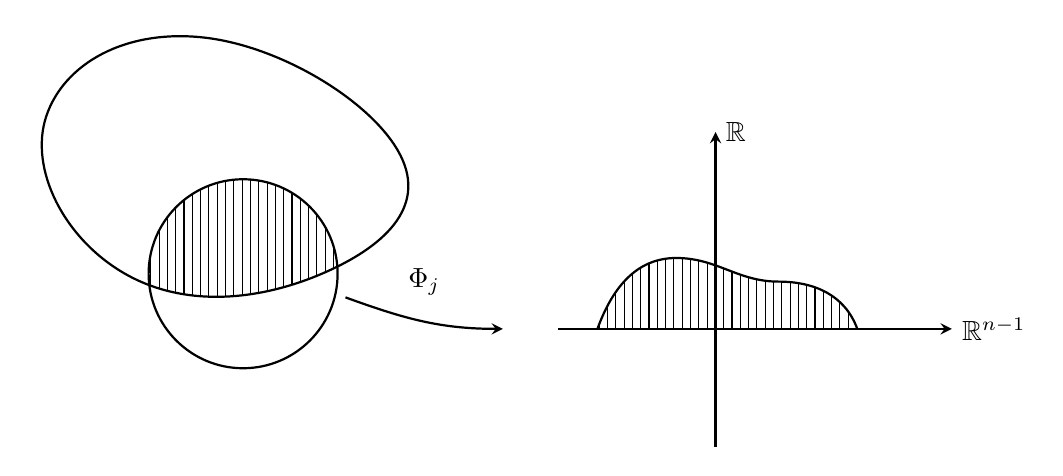
\begin{tikzpicture}[centered]
    % --- 左侧：流形区域与局部邻域 (Domain and local chart) ---
    % 定义区域 \Omega 的边界曲线 (不规则闭合图形)
    \def\domainpath{plot[smooth cycle, tension=0.8] coordinates {(-3, 1.5) (-1, 2.5) (1.5, 1) (0.5, -0.5) (-2, -0.5)}}
    % 定义局部坐标邻域 U_j (圆)
    \def\circlepath{(-0.5, -0.5) circle (1.2cm)}
    % 填充交集区域 \Omega \cap U_j (使用垂直线段阴影)
    \begin{scope}
        \clip \domainpath;
        \fill[pattern=vertical lines, pattern color=black] \circlepath;
    \end{scope}
    % 绘制区域 \Omega 边界
    \draw[thick] \domainpath;
    % 绘制邻域 U_j 边界
    \draw[thick] \circlepath;
    % --- 中间：映射箭头 ---
    % 绘制带弧度的映射箭头 \Phi_j
    \draw[->, thick, >=stealth] (0.8, -0.8) to[out=-20, in=180] (2.8, -1.2);
    \node[above] at (1.8, -0.9) {$\Phi_j$};
    % --- 右侧：局部坐标系下的拉平区域 ---
    \begin{scope}[shift={(5.5, -1.2)}]
        % 横轴 \mathbb{R}^{n-1}
        \draw[->, thick, >=stealth] (-2, 0) -- (3, 0) node[right] {$\mathbb{R}^{n-1}$};
        % 纵轴 \mathbb{R}
        \draw[->, thick, >=stealth] (0, -1.5) -- (0, 2.5) node[right] {$\mathbb{R}$};
        % 映射后的区域边界 (上半空间中的图像)
        \def\mappedpath{(-1.5, 0) to[out=70, in=180] (-0.5, 0.9) to[out=0, in=180] (0.8, 0.6) to[out=0, in=110] (1.8, 0)} 
        % 填充上半区域内的阴影 (垂直线段)
        \fill[pattern=vertical lines, pattern color=black] \mappedpath -- cycle; 
        % 绘制上半部分的边界函数曲线
        \draw[thick] \mappedpath;
    \end{scope}
\end{tikzpicture}

令 $u_{j} = u\eta_{j} \in H^{1}(O_j)$, $v_{j} = u_{j} \circ \Phi_{j}^{-1} \in H^{1}(U_j \cap \mathbb{R}^{n-1} \times \{ x_n > 0 \})$\\
回到上半平面 $v \in H^{1}(\mathbb{R}^{n-1} \times \{ x_n > 0 \})$ 延拓 $v$
\begin{equation*}
    \tilde{v} = \begin{cases}
        v(x', x_n), & x_n > 0\\
        v(x', -x_n), & x_n < 0
    \end{cases}
\end{equation*}
那么有如下Claim: $\tilde{v} \in H^{1}(\mathbb{R}^n)$ . 证明一下这个Claim:
\begin{proof}
    我们的目标是证明 $\tilde{v} \in H^{1}(\mathbb{R}^n)$, 也就是 $\tilde{v} \in L^2(\mathbb{R}^n)$ 且 $\partial_{x_i}\tilde{v} \in L^2(\mathbb{R}^n),\ i=1, 2, \cdots, n$.\\
    首先 $\Vert \tilde{v} \Vert_{L^2(\mathbb{R}^n)} = 2\Vert v \Vert_{L^2(\mathbb{R}^{n}_{+}) }$ 所以 $\tilde{v} \in L^2(\mathbb{R}^n)$.\\
    其次, 对任意的 $1\leq i\leq n$, 要证明 $\partial_{x_i}\tilde{v} \in L^2(\mathbb{R}^n)$, 
    \begin{equation*}
        \partial_{x_i}\tilde{v} = \begin{cases}
            \widetilde{\partial_{x_i}v(x', x_n)}, & 1 \leq i \leq n-1\quad \widetilde{(\cdot)} \text{表示偶延拓}\\
            (\partial_{x_n}v(x', -x_n))^{*}, & i=n\quad (\cdot)^{*} \text{表示奇延拓}
            \end{cases}
    \end{equation*}
    情形1: $1 \leq i \leq n-1$.\par
    对任意的 $\varphi \in C_c^{\infty}(\mathbb{R}^n)$, 有
    $$\langle \partial_{x_i}\tilde{v}, \varphi \rangle = -\langle v, \partial_{x_i}\varphi \rangle$$
    \begin{equation*}
        \begin{aligned}
            \langle \tilde{v}, \partial_{x_i}\varphi \rangle &= \int_{\mathbb{R}^n} \tilde{v(x)} \partial_{x_i}\varphi(x) \mathrm{d}x = \int_{\mathbb{R}^{n}_{+}} v(x) \partial_{x_i}\varphi(x) \mathrm{d}x+\int_{\mathbb{R}^{n}_{-}} v(x) \partial_{x_i}\varphi(x) \mathrm{d}x\\
                                                             &\xlongequal{\text{变量替换}} \int_{\mathbb{R}^{n}_{+}} v(x)\underbrace{\left( \partial_{x_i}\varphi(x', x_n)+\partial_{x_i}\varphi(x', -x_n) \right)}_{\partial_{x_i}\psi} \mathrm{d}x\\
        \end{aligned}
    \end{equation*}
    这里 $\psi \in C_c^{\infty}(\overline{\mathbb{R}^n_{+}})$, 但是不一定属于 $C_c^{\infty}(\mathbb{R}^n)$, 取 $\zeta \in C^{\infty}(\mathbb{R})$ 满足: $0 \leq \zeta \leq 1$ 且
    \begin{equation*}
        \zeta(t) = \begin{cases}
            1, & t \geq 2\\
            0, & t \leq 1
        \end{cases}
    \end{equation*}
    记 $\psi_{k} = \zeta(kx_n)\psi(x)$, 则 $\supp(\psi_{k}) = \mathbb{R}^{n-1}\times [\frac{1}{k},\infty) \subset \mathbb{R}^n_{+}$. 所以可以得到 $\psi_k \in C_c^{\infty}(\mathbb{R}^n_{+})$.
    \begin{equation*}
        \begin{aligned}
            \int_{\mathbb{R}^{n}_{+}} v(x)\partial_{x_i}\psi(x) \mathrm{d}x &= \langle v, \partial_{x_i}\psi \rangle = - \langle \partial_{x_i}v, \psi_k \rangle 
                                                                            &= -\int_{\mathbb{R}^{n}_{+}} \partial_{x_i}v(x)\psi_k(x) \mathrm{d}x 
        \end{aligned}
    \end{equation*}
    由控制收敛定理:
    \begin{equation*}
        \text{左式} \xlongrightarrow{k \to \infty} -\int_{\mathbb{R}^{n}_{+}} v(x)\partial_{x_i}\psi(x) \mathrm{d}x 
    \end{equation*}
    \begin{equation*}
        \text{右式}= -\int_{\mathbb{R}^{n}_{+}} \partial_{x_i}v(x)\psi(x) \mathrm{d}x
    \end{equation*}
    从而有 $\langle \tilde{v}, \partial_{x_i}\varphi \rangle = -\langle \widetilde{\partial_{x_i}v}, \varphi \rangle$. 进而 $\tilde{v} \in L^{2}(\mathbb{R}^n)$.\\
    情形2: $i=n$.\par
    对任意的 $\varphi \in C_c^{\infty}(\mathbb{R}^n)$, 有
    $$\langle \partial_{x_n}\tilde{v}, \varphi \rangle = -\langle v, \partial_{x_n}\varphi \rangle$$
    \begin{equation*}
        \begin{aligned}
            \langle \tilde{v}, \partial_{x_n}\varphi \rangle &= \int_{\mathbb{R}^n} \tilde{v(x)} \partial_{x_n}\varphi(x) \mathrm{d}x = \int_{\mathbb{R}^{n}_{+}} v(x) \partial_{x_n}\varphi(x) \mathrm{d}x+\int_{\mathbb{R}^{n}_{-}} v(x) \partial_{x_n}\varphi(x) \mathrm{d}x\\
                                                             &\xlongequal{\text{变量替换}} \int_{\mathbb{R}^{n}_{+}} v(x)\underbrace{\left( \partial_{x_n}\varphi(x', x_n)+\partial_{x_n}\varphi(x', -x_n) \right)}_{\partial_{x_n}\tilde{\psi}} \mathrm{d}x\\
        \end{aligned}
    \end{equation*}
    这里 $\tilde{\psi} \in C_c^{\infty}(\overline{\mathbb{R}^n_{+}})$, 但是不一定属于 $C_c^{\infty}(\mathbb{R}^n)$, 取 $\zeta \in C^{\infty}(\mathbb{R})$ 满足: $0 \leq \zeta \leq 1$ 且
    \begin{equation*}
        \zeta(t) = \begin{cases}
            1, & t \geq 2\\
            0, & t \leq 1
        \end{cases}
    \end{equation*}
    记 $\tilde{\psi}_{k} = \zeta(kx_n)\tilde{\psi}(x)$, 则 $\supp(\tilde{\psi}_{k}) = \mathbb{R}^{n-1}\times [\frac{1}{k},\infty) \subset \mathbb{R}^n_{+}$. 所以可以得到 $\tilde{\psi}_k \in C_c^{\infty}(\mathbb{R}^n_{+})$.
    \begin{equation*}
        \begin{aligned}
            \int_{\mathbb{R}^{n}_{+}} v(x)\partial_{x_n}\tilde{\psi}(x) \mathrm{d}x &= \langle v, \partial_{x_n}\tilde{\psi} \rangle = - \langle \partial_{x_n}v, \tilde{\psi}_k \rangle\\
        \end{aligned}
    \end{equation*}
    \begin{equation*}
        \text{右式}=-\int_{\mathbb{R}^{n}_{+}} \partial_{x_n}v(x)\zeta(kx_n)\tilde{\psi}(x) \mathrm{d}x \xlongrightarrow{\text{DCT}}-\int_{\mathbb{R}^{n}_{+}} \partial_{x_n}v(x)\tilde{\psi}(x) \mathrm{d}x
    \end{equation*}
    \begin{equation*}
        \text{左式}=\int_{\mathbb{R}^{n}_{+}} v(x)\zeta(kx_n)\partial_{x_n}\tilde{\psi}(x) \mathrm{d}x + \int_{\mathbb{R}^{n}_{+}} v(x)\zeta'(kx_n)k\tilde{\psi}(x) \mathrm{d}x = J_1 + J_2
    \end{equation*}
    \begin{equation*}
        J_{1} \xlongrightarrow{\text{DCT}} \int_{\mathbb{R}^{n}_{+}} v(x)\partial_{x_n}\tilde{\psi}(x) \mathrm{d}x
    \end{equation*}
    由于 $\zeta'(kx_{n})$ 在 $x_{n} \in [\frac{1}{k},\frac{2}{k}]$ 上非零, 且 $\tilde{\psi}$ 关于 $x_{n}$ 是奇函数, 所以我们有增量估计 $|\tilde{\psi}|\leq C|x_n|$, 且
    $\supp(\tilde{\psi}) \subset B_{R}(0)$, 从而
    \begin{equation*}
        \begin{aligned}
            |J_{2}| &\leq \int_{B_{R}(0) \cap \{x_n \in [\frac{1}{k},\frac{2}{k}]\}} |v(x)| |\zeta'(kx_n)| k C|x_{n}| \mathrm{d}x\\
                    &\leq C' \int_{B_{R}(0) \cap \{x_n \in [\frac{1}{k},\frac{2}{k}]\}} |v(x)| \mathrm{d}x \xlongrightarrow{k \to \infty} 0
        \end{aligned}
    \end{equation*}
    所以我们有结论: 
    \begin{equation*}
        -\int_{\mathbb{R}^{n}_{+}} v(x)\partial_{x_n}\tilde{\psi}(x) \mathrm{d}x = -\int_{\mathbb{R}^{n}_{+}} \partial_{x_n}v(x)\tilde{\psi}(x) \mathrm{d}x
    \end{equation*}
    即:
    \begin{equation*}
        -\int_{\mathbb{R}^{n}} (\partial_{x_n}v)^{*} \varphi \mathrm{d}x = \int_{\mathbb{R}^{n}}v^{*} \partial_{x_n}\varphi \mathrm{d}x
    \end{equation*}
    这也说明了 $\forall 1 \leq i \leq n$, 有 $\partial_{x_i}\tilde{v} \in L^{2}(\mathbb{R}^n)$, 进而说明 $\tilde{v} \in H^{1}(\mathbb{R}^n)$.
\end{proof}
由上述Claim 我们可以得到: $\forall v \in H^{1}(\mathbb{R}^n_{+})$, 通过关于 $x_{n}$ 的偶延拓 $\tilde{v} \in H^{1}(\mathbb{R}^n)$. 故我们可以通过 $\tilde{v}$ 的迹来定义 $v$ 在 $\mathbb{R}^{n-1}\times \{0\}$ 上的迹. 
$\gamma v$ 或者 $v|_{\mathbb{R}^{n-1}\times \{0\}}$ 称为 $v$ 在 $\partial \mathbb{R}^{n}_{+} = \mathbb{R}^{n-1}\times \{0\}$ 上的迹. $\gamma v \in H^{1/2}(\mathbb{R}^{n-1})$. 进一步的
\begin{enumerate}
    \item $C_{c}^{\infty}(\mathbb{R}^n_{+})$ 在 $H^{1}(\mathbb{R}^n_{+})$ 中稠密;
    \item 分部积分公式成立;
    \item $ \gamma: H^{1}(\mathbb{R}^n_{+}) \longrightarrow H^{1/2}(\mathbb{R}^{n-1}) $ 是连续线性映射.
\end{enumerate}
接下来回到光滑有界区域 $\Omega$, 对 $v_{j}\in H^{1}(\mathbb{R}^{n}_{+})$ 那么 $u|_{\partial \Omega} = \sum\limits_{j=1}^{n} \gamma v_j \circ \Phi_j^{-1}$ 称为
$u$ 在 $\partial \Omega$ 上的迹. $\Vert u \Vert_{H^{1/2}(\partial \Omega)}^{2} = \sum\limits_{j=1}^{n} \Vert \gamma v_j  \Vert_{H^{1/2}(\mathbb{R}^{n}_{+})}^{2}$. 
那么实际上这个范数等价于:
\begin{equation*}
    \Vert u \Vert_{H^{1/2}(\partial \Omega)}^{2} = \int_{\partial \Omega \times \partial \Omega} \frac{|u(x)-u(y)|^2}{|x-y|^n} \mathrm{d}\sigma(x)\mathrm{d}\sigma(y) 
\end{equation*}
同样的有: 
\begin{enumerate}
    \item $C_{c}^{\infty}(\Omega)$ 在 $H^{1}(\Omega)$ 中稠密;
    \item $ \gamma: H^{1}(\Omega) \longrightarrow H^{1/2}(\partial \Omega) $ 是连续线性满射;
    \item 分部积分公式在 $H^{1}(\Omega)$ 中成立 即 $\forall w, v \in H^{1}(\Omega)$,
    \begin{equation*}
        \int_{\Omega}\partial_{x_i}v w \mathrm{d}x = -\int_{\Omega} v \partial_{x_i}w \mathrm{d}x + \int_{\partial \Omega} v w \nu_i \mathrm{d}\sigma
    \end{equation*}
\end{enumerate}
\subsection{$H_{0}^{1}(\Omega)$}
\begin{definition}
    $H_{0}^{1}(\Omega) $, 是 $\mathscr{D}(\Omega)$ 在 $H^{1}(\Omega)$ 中的闭包. $H_{0}^{1}(\Omega) = \overline{\mathscr{D}(\Omega)}^{H^{1}(\Omega)}$
\end{definition}
\begin{remark}
    $H_{0}^{1}(\Omega)\subsetneq H^{1}(\Omega)$. 比如非零常值函数 $u(x) = 1$ 在 $\Omega$ 中属于 $H^{1}(\Omega)$, 但是不属于 $H_{0}^{1}(\Omega)$.
\end{remark}
对于 $H_{0}^{1}(\Omega)$, 我们有如下对其的刻画:
\begin{theorem}
    设 $\Omega$ 为一光滑有界区域,$u \in H^{1}(\Omega)$ 则以下性质等价:
    \begin{enumerate}
        \item $u \in H_{0}^{1}(\Omega)$;
        \item $u$ 在 $\partial \Omega$ 上的迹为零, 即 $\gamma u = 0$;
        \item $u \mathbbm{1}_{\Omega} \in H^{1}(\mathbb{R}^n)$
    \end{enumerate}
\end{theorem}
\begin{proof}\par
    $\bullet (1) \Rightarrow (2)$ 是平凡的.\\
    $\bullet (2) \Rightarrow (3)$.\par
    记 $\tilde{u} = u \mathbbm{1}_{\Omega}$, 则 $\Vert \tilde{u} \Vert_{L^2(\mathbb{R}^n)} = \Vert u \Vert_{L^2(\Omega)} < \infty$.\\
    其次, 对任意的 $\varphi \in \mathscr{D}(\mathbb{R}^n)$, 有
    \begin{equation*}
        \begin{aligned}
            \langle \partial_{x_i}\tilde{u}, \varphi \rangle &= -\langle \tilde{u}, \partial_{x_i}\varphi \rangle = -\int_{\Omega} u(x) \partial_{x_i}\varphi(x) \mathrm{d}x\\
            &\xlongequal{\text{分部积分}} \int_{\Omega} \partial_{x_i}u(x) \varphi(x) \mathrm{d}x - \int_{\partial \Omega} u(x) \varphi(x) \nu_i \mathrm{d}\sigma \\
            &= \int_{\Omega} \partial_{x_i}u(x) \varphi(x) \mathrm{d}x\\
            & = \int_{\mathbb{R}^n} \partial_{x_i}u(x) \mathbbm{1}_{\Omega}(x) \varphi(x) \mathrm{d}x
        \end{aligned}
    \end{equation*}
    所以有 $\partial_{x_i}\tilde{u} = \partial_{x_i}u \mathbbm{1}_{\Omega}$ 在 $L^2(\mathbb{R}^n)$ 中. 从而 $\tilde{u} \in H^{1}(\mathbb{R}^n)$.\\
    $\bullet (3) \Rightarrow (1)$.\par
    利用单位分解, $u = \sum\limits_{j=1}^{n} \eta_{j} u = \sum\limits_{j=1}^{n} u_{j}$, 其中 $\eta_{j} \in C_c^{\infty}(\Omega_j)$ 且 $\sum\limits_{j=1}^{N} \varphi_j = 1$ 在 $\Omega$ 上, 且
    $\supp(\eta_j) \subset U_{j}$.\\
    \textbf{情形1}: $\overline{U_{j}} \subset \Omega$. 我们考虑卷积 $u_{j} * \xi_{\varepsilon}$, 则 $\supp(u_{j} * \xi_{\varepsilon}) \subset U_{j} \subset \Omega$, $\varepsilon$ 充分小.
    进而由卷积的性质 $u_{j} * \xi_{\varepsilon} \in C_c^{\infty}(\Omega)$, 且 $u_{j} * \xi_{\varepsilon} \xlongrightarrow{\varepsilon \to 0} u_{j}$ 在 $H^{1}(\Omega)$ 中.\\
    \textbf{情形2}: $\overline{U_{j}} \cap \partial \Omega \neq \varnothing$. 选取适当的微分同胚 $\Phi_{j}$ 将 $U_{j}$ 映射到 $V_{j} \subset \mathbb{R}^{n}$ 上, 令 $w_{j} = u_{j}\mathbbm{1}_{\Omega} \circ \Phi_{j}^{-1} \in H^{1}(\mathbb{R}^n)$,
    且 $\supp(w_j) \subset \overline{\mathbb{R}^{n}_{+}}$. 考虑平移 $v_{\varepsilon} = w_{j}(x', x_n - \varepsilon), \varepsilon > 0$. 此时
    $\supp(v_{\varepsilon}) \subset \mathbb{R}^{n-1}\times [\varepsilon, \infty)$.\par
    固定上述 $\varepsilon$, 再考虑卷积 $v_{\varepsilon} * \xi_{\delta}$, 其中 $\xi_{\delta}$ 是一个光滑的截断函数. 则 $\supp(v_{\varepsilon} * \xi_{\delta}) \subset \mathbb{R}^{n}_{+}(\delta < \varepsilon)$. 则有:
    \begin{equation*}
        (v_{\varepsilon} * \xi_{\delta}) \circ \Phi_{j} \in C_c^{\infty}(\Omega) \xlongrightarrow{\delta \to 0} v_{\varepsilon} \circ \Phi_{j} = u_{j}\mathbbm{1}_{\Omega}(x', x_n - \varepsilon) \xlongrightarrow{\varepsilon \to 0} u_{j}\mathbbm{1}_{\Omega} = u_{j}
    \end{equation*}
    故可以用 $C_c^{\infty}(\Omega)$ 函数在 $H^{1}(\Omega)$ 中逼近 $u_{j}$. 这就说明了 $u_{j} \in H_{0}^{1}(\Omega)$. 从而 $u = \sum\limits_{j=1}^{n} u_{j} \in H_{0}^{1}(\Omega)$.
\end{proof}
接下来介绍Friedrichs-Poincaré不等式:\par
设 $\Omega \subset \mathbb{R}^n$ 是一个光滑有界区域, 则在 $H_{0}^{1}(\Omega)$ 中 $\Vert u \Vert_{H^1(\Omega)}$ 和 $\Vert \nabla u \Vert_{L^2(\Omega)}$ 是等价的. 
\begin{remark}
    设 $E$ 为一线性空间, $\Vert \cdot \Vert_{1}$ 和 $\Vert \cdot \Vert_{2}$ 是 $E$ 上的两个范数. 如果存在 $C_{1}, C_{2} > 0$ 使得 $\forall x \in E, C_{1}\Vert x \Vert_{1} \leq \Vert x \Vert_{2}\leq C_{2}\Vert x \Vert_{1} $ 
    则称 $\Vert \cdot \Vert_{1}$ 和 $\Vert \cdot \Vert_{2}$ 是等价的. 
\end{remark}
\begin{proof}
    首先 $\Vert \nabla u \Vert_{L^2} \leq \Vert u \Vert_{H^{1}}$ 是平凡的. 下面证明存在 $C > 0$ 使得 
    \begin{equation}\label{Friedrichs-Poincaré inequality}
        \Vert u \Vert_{H^{1}} \leq C\Vert \nabla u \Vert_{L^2}
    \end{equation}
    这个不等式就是Friedrichs-Poincaré不等式.\par
    设 $\Omega \subset (a,b)\times \mathbb{R}^{n-1}$ 是一个光滑有界区域. 任取 $u \in \mathscr{D}(\Omega)$, 那么由Newton-Leibniz公式:
    \begin{equation*}
        u(x) = u(x',a)+\int_{a}^{x_n} \partial_{x_n}u(x', s) \mathrm{d}s
    \end{equation*}
    进而
    \begin{equation*}
        \begin{aligned}
            |u(x)|^{2} &\leq \left( \int_{a}^{x_{n}}\left| \frac{\partial u}{\partial x_{n}}(x', s) \right| \mathrm{d}s \right)^2\quad \text{(因为 $u(x', a) = 0$)}\\
            &\leq (x_{n}-a)^2 \int_{a}^{x_{n}} \left|\frac{\partial u}{\partial x_{n}}(x', s) \right|^2 \mathrm{d}s \quad \text{(Cauchy-Schwarz不等式)}\\
            &\leq (b-a)^2 \int_{a}^{b} \left|\frac{\partial u}{\partial x_{n}}(x', s) \right|^2 \mathrm{d}s\\
            & \Longrightarrow \int_{a}^{b} |u(x)|^2 \mathrm{d}x_n \leq (b-a)^2 \int_{a}^{b} \left|\frac{\partial u}{\partial x_{n}}(x', s) \right|^2 \mathrm{d}s
        \end{aligned}
    \end{equation*}
    接下来对 $x'$ 积分:
    \begin{equation*}
        \Vert u \Vert_{L^2((a,b)\times \mathbb{R}^{n-1})}^2 \leq (b-a)^2 \Vert \nabla u \Vert_{L^2((a,b)\times \mathbb{R}^{n-1})}^2
    \end{equation*}
    从而对任意的 $u \in \mathscr{D}(\Omega)$ 成立:
    \begin{equation*}
        \Vert u \Vert_{L^2(\Omega)} \leq \Vert u \Vert_{L^2((a,b)\times \mathbb{R}^{n-1})} \leq (b-a) \Vert \nabla u \Vert_{L^2((a,b)\times \mathbb{R}^{n-1})} \leq (b-a) \Vert \nabla u \Vert_{L^2(\Omega)}
    \end{equation*}
    即在 $\mathscr{D}(\Omega)$ 中成立Friedrichs-Poincaré不等式(\ref{Friedrichs-Poincaré inequality}). 由 $\mathscr{D}(\Omega)$ 在 $H_{0}^{1}(\Omega)$ 中的稠密性, 可以得到在 $H_{0}^{1}(\Omega)$ 中也成立Friedrichs-Poincaré不等式.
\end{proof}
接下来介绍Sobolev紧嵌入定理:\par
\begin{theorem}
    设 $\Omega \subset \mathbb{R}^n$ 是一个光滑有界区域, 则 $H_{0}^{1}(\Omega)$ 紧嵌入 $L^2(\Omega)$. 记为 $H_{0}^{1}(\Omega) \hookrightarrow\hookrightarrow L^2(\Omega)$.
\end{theorem}
\begin{remark}
    设 $(E,d_{1}),(F,d_{2})$ 是两个度量空间, 我们称映射 $T: E \longrightarrow F$ 是紧映射, 如果对于任意的 $A \subset E$ 有界, 则 $T(A)$ 在 $F$ 中是相对紧的.即
    $\overline{T(A)}$ 是紧的. 换言之, $\forall$ 有界序列 $\{ x_{k}\} \subset T(A)$ 则存在子列 $\{ x_{n_{p}} \}$ 使得 $x_{n_{p}} \xlongrightarrow{p \to \infty} x$ 在 $F$ 中. 这也说明了紧映射是连续的.
\end{remark}
\begin{remark}
    在度量空间中: 
    \begin{equation*}
        \text{紧性} \Longleftrightarrow  \text{序列紧} \Longleftrightarrow\text{预紧+完备}
    \end{equation*}
    从而在完备的度量空间中, 相对紧性等价于预紧性. 
\end{remark}
\begin{definition}[预紧性]
    $A \subset (E,d)$ 是预紧的, 如果对于任意的 $\varepsilon > 0$, 存在有限集 $\{ x_{p} \}$ 使得 $A \subset \bigcup\limits_{p} B_{\varepsilon}(x_{p})$.
\end{definition}
接下来证明紧嵌入定理
\begin{proof}
    我们的目标是去证明 $H_{0}^{1} \xlongrightarrow{\operatorname{id}}L^2$ 是一个紧映射.\par
    因为上述映射是一个线性映射, 故只需证明对单位球 $B_{H_{0}^{1}} \subset H_{0}^{1}(\Omega)$, $B_{H_{0}^{1}}$ 在 $L^2(\Omega)$ 中是预紧或者相当紧的.\par
    $\forall u \in H_{0}^{1}(\Omega)$, 则 $u\cdot \mathbbm{1}_{\Omega} \in H_{0}^{1}(\mathbb{R}^n)$. 故取开集 $U \supset \Omega\text{的1-邻域}$.
    设 $u \in H_{0}^{1}(U)$ , 则有 $\supp(u) \subset \Omega$.\par
    取磨光子 $\xi \in C_{c}^{\infty}(B)$ 使得 $\xi \geq 0, \int_{B} \xi(x) \mathrm{d}x = 1, \xi_{\delta}(x) = \frac{1}{\delta^n}\xi\left(\frac{x}{\delta}\right)$. 这里$B$ 是包含在$U$ 里的一个开球.
    考虑 $u_{\delta} = u \ast \xi_{\delta}$, 下设 $u \in \mathscr{D}(\Omega)$
    \begin{equation*}
        \begin{aligned}
            u(x) - u_{\delta}(x) &= u(x) - \int_{\mathbb{R}^n} u(x-y)\xi_{\delta}(y) \mathrm{d}y\\
                                 &= \int_{\mathbb{R}^n} (u(x) - u(x-y))\xi_{\delta}(y) \mathrm{d}y\\
                                 &= \int_{\mathbb{R}^n} \left( \int_{0}^{1} \nabla u(x-ty) \cdot y \mathrm{d}t \right) \xi_{\delta}(y) \mathrm{d}y\\ \quad(Newton-Leibniz公式)
        \end{aligned}
    \end{equation*}
    进而
    \begin{equation*}
        \begin{aligned}
            |u(x) - u_{\delta}(x)|^{2}  &\leq \left( \int_{\mathbb{R}^n} \left| \int_{0}^{1} \nabla u(x-ty) \cdot y \mathrm{d}t \right|\xi_{\delta} \mathrm{d}y \right)^2\\
                                        &\leq \left( \int_{\mathbb{R}^n} \int_{0}^{1} |\nabla u(x-ty)| |y|\xi_{\delta} \mathrm{d}t \mathrm{d}y \right)^2\\
                                        &\leq \left( \int_{\mathbb{R}^n} \int_{0}^{1} |\nabla u(x-ty)||y|\frac{1}{\delta^{n}}\xi\left(\frac{y}{\delta}\right) \mathrm{d}t \mathrm{d}y \right)^2\\
                                        &\xlongequal{y=\delta z} \left( \int_{\mathbb{R}^n} \int_{0}^{1} |\nabla u(x-t\delta z)| \delta|z| \xi(z) \mathrm{d}t \mathrm{d}z \right)^2\\
                                        &\leq C\delta^{2} \left( \int_{B} \int_{0}^{1} |\nabla u(x-t\delta z)|^2 \mathrm{d}t \mathrm{d}z \right)^{2}\\
                                        &\leq C\delta^2|B| \int_{B} \int_{0}^{1} |\nabla u(x-t\delta z)|^2 \mathrm{d}t \mathrm{d}z \quad \text{(Cauchy-Schwarz不等式)}\\
        \end{aligned}
    \end{equation*}
    \begin{equation*}
        \begin{aligned}
            \int_{\mathbb{R}^{n}} |u(x) - u_{\delta}(x)|^2 \mathrm{d}x  &\leq C'\delta^2 \int_{\mathbb{R}^n} \int_{B} \int_{0}^{1} |\nabla u(x-t\delta z)|^2 \mathrm{d}t \mathrm{d}z \mathrm{d}x\\
                                                                        &\xlongequal{\text{Fubini}} C'\delta^2 \int_{B} \int_{0}^{1} \underbrace{\int_{\mathbb{R}^n} |\nabla u(x-t\delta z)|^2 \mathrm{d}x}_{\Vert \nabla u \Vert_{L^2(\mathbb{R}^n)}^2} \mathrm{d}t \mathrm{d}z\\
                                                                        &= M\delta^2 \Vert \nabla u \Vert_{L^2(\mathbb{R}^n)}^2 = M\delta^2 \Vert u \Vert_{L^2(\Omega)}^2
        \end{aligned}
    \end{equation*}
    所以我们得到结论: 对任意的 $\delta \in (0,1)$, 有 $\Vert u - u \ast \xi_{\delta} \Vert_{L^2(\Omega)} \leq C\delta \Vert \nabla u \Vert_{L^2(\Omega)},\ \forall u \in \mathscr{D}(\Omega)$.
    由 $\mathscr{D}(\Omega)$ 在 $H_{0}^{1}(\Omega)$ 中稠密, 我们可以将上述不等式延拓到整个 $H_{0}^{1}(\Omega)$ 上.\par
    取定 $\varepsilon > 0, \forall u \in B_{H_{0}^{1}}$, $\Vert u - u_{\delta} \Vert_{L^2(\Omega)} < M\delta \xlongequal{\text{取}\delta = \frac{\varepsilon}{2M}} \varepsilon/2$.\par
    接下来只需证明: $\{ u_{\delta} : u \in B_{H_{0}^{1}} \}$ 在 $L^2(\Omega)$ 中是相对紧的.\par
    我们将会使用 Arzelà-Ascoli定理来证明 $\{ u_{\delta} : u \in B_{H_{0}^{1}} \}$ 在 $L^2(\Omega)$ 中是相对紧的.\par
    \begin{equation*}
        \begin{aligned}
            |u_{\delta}(x)|^{2} = |u \ast \xi_{\delta}(x)|^2    &= \left( \int_{\Omega} u(y)\xi_{\delta}(x-y) \mathrm{d}y \right)^2 \leq \left( \int_{\Omega} |u(y)|\frac{1}{\delta^n}\xi\left(\frac{x-y}{\delta}\right) \mathrm{d}y \right)^2\\
                                                                &\leq \frac{C}{\delta^{2n}}\left( \int_{\Omega} |u(y)| \mathrm{d}y \right)^2 \leq \frac{C}{\delta^{2n}}|\Omega|\int_{\Omega} |u(y)|^2 \mathrm{d}y\\
                                                                &\leq \frac{C}{\delta^{2n}}|\Omega| \Vert u \Vert_{L^2(\Omega)}^2 \leq \frac{C'}{\delta^{2n}}\Vert u \Vert_{H_{0}^{1}(\Omega)}^2 \leq \frac{C'}{\delta^{2n}}
        \end{aligned}
    \end{equation*}
    从而 $u_{\delta}$ 是一致有界的.\par
    那么只需证明 $u_{\delta}$ 是等度连续的即可, 这等价于证明 $u_{\delta}$ 是一致Lipschitz连续的, 为了证明一致Lipschitz连续我们只需要证明 $\nabla u_{\delta}$ 是一致有界的.\par
    由于 $\nabla u_{\delta} = (\nabla u) \ast  \xi_{\delta}$, 同上我们可以得到 $\nabla u_{\delta}$ 是一致有界的. 从而 $u_{\delta}$ 是一致Lipschitz连续的. 
    由Arzelà-Ascoli定理, 对于 $\delta = \frac{\varepsilon}{2M}$, $\{ u_{\delta} : u \in B_{H_{0}^{1}} \}$ 在 $\Vert \cdot \Vert_{\infty}$ 下是相对紧的, 从而是预紧的.\par
    又由于 $|\Omega| < \infty$, $\Vert f \Vert_{L^2(\Omega)} < \sqrt{|\Omega|}\Vert f \Vert_{L^\infty(\Omega)}$, 从而 $\{ u_{\delta} : u \in B_{H_{0}^{1}} \}$ 在 $\Vert \cdot \Vert_{L^2(\Omega)}$ 下也是预紧的.
    这说明 $\{ u_{\delta}\ :\ u \in B_{H_{0}^{1}} \}$ 可以被有限个半径为 $\varepsilon/2$ 的 $L^2$ 球覆盖. 从而 $\{ u : u \in B_{H_{0}^{1}} \}$ 可以被有限个半径为 $\varepsilon$ 的 $L^2$ 球覆盖. 这说明 $B_{H_{0}^{1}}$ 在 $L^2(\Omega)$ 中是预紧的, 从而 $H_{0}^{1}(\Omega) \hookrightarrow\hookrightarrow L^2(\Omega)$.
\end{proof}
\subsection{求解Laplace方程}
接下来我们介绍怎么在Sobolev空间中去求解Laplace方程. 设 $\Omega \subset \mathbb{R}^n$ 是一个光滑有界区域, $f \in L^2(\Omega)$, 则我们想要去求解如下的边值问题:
\begin{equation*}
    (L)
    \begin{cases}
        -\Delta u = f, & \text{in } \Omega\\
        u = 0, & \text{on } \partial \Omega
    \end{cases}
\end{equation*}
和之前一样由于线性性我们可以分解成两个方程:
\begin{equation*}
    (L_1)
    \begin{cases}
        -\Delta u = f, & \text{in } \Omega\\
        u = 0, & \text{on } \partial \Omega
    \end{cases}
    \qquad\qquad
    (L_2)
    \begin{cases}
        -\Delta u = 0, & \text{in } \Omega\\
        u = g, & \text{on } \partial \Omega
    \end{cases}
\end{equation*}
先看 $(L_1)$, 设 $(L_1)$ 在分布意义下有解, 那么对于任意的检验函数 $\varphi \in \mathscr{D}(\Omega)$, 有
\begin{equation*}
    \langle -\Delta u, \varphi \rangle = \langle f, \varphi \rangle = \int_{\Omega} f(x) \varphi(x) \mathrm{d}x
\end{equation*}
那么由分布的分部积分上述左式可以变成:
\begin{equation*}
    \langle -\Delta u, \varphi \rangle = \langle \nabla u, \nabla \varphi \rangle \xlongequal{\text{若}u \in H^{1}(\Omega)} \int_{\Omega} \nabla u(x) \cdot \nabla \varphi(x) \mathrm{d}x
\end{equation*}
所以, 若 $u \in H_{0}^{1}(\Omega)$, 则有
\begin{equation*}
    \int_{\Omega} \nabla u(x) \cdot \nabla \varphi(x) \mathrm{d}x = \int_{\Omega} f(x) \varphi(x) \mathrm{d}x
\end{equation*}
\begin{remark}
    \begin{equation*}
        \int_{\Omega} \nabla u(x) \cdot \nabla \varphi(x) \mathrm{d}x = \langle \nabla u, \nabla \varphi \rangle \xlongequal{\text{Friedrichs-Poincaré不等式}} \langle u, \varphi \rangle_{H_{0}^{1}(\Omega)}
    \end{equation*}
\end{remark}
所以方程的求解变成了证明
\begin{equation*}
    \forall \varphi \in H_{0}^{1}(\Omega),\ \langle u, \varphi \rangle_{H_{0}^{1}(\Omega)} = \int_{\Omega} f(x) \varphi(x) \mathrm{d}x
\end{equation*}
我们有如下命题:
\begin{proposition}
    设 $\Omega \subset \mathbb{R}^n$ 是一个光滑有界区域, 则对于任意的 $f \in L^2(\Omega)$, 存在唯一的 $u \in H_{0}^{1}(\Omega)$ 使得 $\forall \varphi \in H_{0}^{1}(\Omega),\ \langle u, \varphi \rangle_{H_{0}^{1}(\Omega)} = \int_{\Omega} f(x) \varphi(x) \mathrm{d}x$.
\end{proposition}
\begin{proof}
    令 $l(\varphi) = \int_{\Omega} f(x) \varphi(x) \mathrm{d}x$. 则 $l \in (H_{0}^{1}(\Omega))'$.
    由 Riesz表示定理, 存在唯一的 $u \in H_{0}^{1}(\Omega)$ 使得$\forall \varphi \in H_{0}^{1}(\Omega)$,
    $$l(\varphi) = \langle u, \varphi \rangle_{H_{0}^{1}(\Omega)}\quad\quad (L_{1}^*).$$ 
    特别的, 取 $\varphi \in \mathscr{D}(\Omega)$ 得到 $-\Delta u \xlongequal{\mathscr{D}} f$.
\end{proof}
\begin{remark}
    我们称 $(L_1^*)$ 为方程 $(L_1)$ 的弱形式(或变分形式). 由弱形式的正则性理论, 如果 $\Omega$ 充分光滑, 可以证明 $u \in H^2(\Omega) \cap H_0^1(\Omega)$.
\end{remark}
再来看 ($L_2$), 设 $u \in H^{1}(\Omega)$ 是 $(L_2)$ 的一个解, 则此时要求 $g \in H^{1/2}(\partial \Omega)$, 这是方程有解的必要条件. 反过来, 
设 $g \in H^{1/2}(\partial \Omega)$, 则存在 $u_{0} \in H^{1}(\Omega)$ 使得 $\gamma u_0 = g$. 这是方程有解的必要条件.
设 $v = u-u_0$, 则 $v$ 满足如下的方程:
\begin{equation*}
    \begin{cases}
        -\Delta v = \Delta u_0, & \text{in } \Omega\\
        v = 0, & \text{on } \partial \Omega
    \end{cases}
\end{equation*}
对任意的 $\varphi \in \mathscr{D}(\Omega)$(由稠密性可以改为 $\varphi \in H_{0}^{1}(\Omega)$), 有
\begin{equation*}
    (L_2')\quad \langle v, \varphi \rangle_{H_{0}^{1}(\Omega)} = \int_{\Omega} \nabla v(x) \cdot \nabla \varphi(x) \mathrm{d}x = -\int_{\Omega} \nabla u_0(x) \cdot \nabla \varphi(x) \mathrm{d}x=l_{0}(\varphi) \Longrightarrow l_{0} \in (H_{0}^{1}(\Omega))'
\end{equation*}
由Riesz表示定理, 存在唯一的 $v \in H_{0}^{1}(\Omega)$ 使得 $\forall \varphi \in H_{0}^{1}(\Omega),\ \langle v, \varphi \rangle_{H_{0}^{1}(\Omega)} = l_{0}(\varphi)$. 从而 $u = u_0 + v$ 是 $(L_2)$ 的一个解.\par
接下来从变分法的角度来看弱形式($L_{1}^*$). 我们将方程的弱形式看成泛函求临界点的问题. 设
\begin{equation*}
    \mathcal{J}(v) = \frac{1}{2}\int_{\Omega} |\nabla v(x)|^2 \mathrm{d}x - \int_{\Omega} f(x) v(x) \mathrm{d}x
\end{equation*}
对其求Frechet导数, 则 
\begin{equation*}
    \partial_{\varphi} \mathcal{J}(v) = \lim\limits_{t \to 0} \frac{\mathcal{J}(v+t\varphi) - \mathcal{J}(v)}{t} = \int_{\Omega} \nabla v(x) \cdot \nabla \varphi(x) \mathrm{d}x - \int_{\Omega} f(x) \varphi(x) \mathrm{d}x 
\end{equation*}
从而 $(L_{1})$ 有解就等价于 $\partial_{\varphi} \mathcal{J}(v) = 0$ 对任意的 $\varphi \in H_{0}^{1}(\Omega)$ 成立. 这也意味着 $\mathcal{J}$ 在 $H_{0}^{1}(\Omega)$ 中的临界点就是 $(L_{1})$ 的解. 
由于 $\mathcal{J}$ 是一个严格凸的泛函, 从而 $(L_{1})$ 的解也是 $\mathcal{J}$ 的唯一的全局最小点. 所以唯一性是平凡的, 我们需要证明存在性, 也就是:
\begin{equation*}
    \inf\limits_{H_{0}^{1}(\Omega)} \mathcal{J}(v)>-\infty \text{且达到该下界}
\end{equation*}
\begin{proof}
    \begin{equation*}
        \begin{aligned}
            \mathcal{J}(v) = \frac{1}{2}\Vert \nabla v \Vert_{L^2(\Omega)}^2 - \int_{\Omega} f(x) v(x) \mathrm{d}x &\geq \frac{1}{2}\Vert \nabla v \Vert_{L^2(\Omega)}^2 - \Vert f \Vert_{L^2(\Omega)}\Vert v \Vert_{L^2(\Omega)}\\
            &\geq  \frac{1}{2}\Vert \nabla v \Vert_{L^2(\Omega)}^2 - C\Vert f \Vert_{L^2(\Omega)}\Vert \nabla v \Vert_{L^2(\Omega)} \quad \text{(Friedrichs-Poincaré不等式)}\\
            &\geq \frac{1}{4}\Vert \nabla v \Vert_{L^2(\Omega)}^2 - \underbrace{C'\Vert f \Vert_{L^2(\Omega)}^2}_{M} \quad \text{(Young不等式)}\\
            &\geq -M > -\infty
        \end{aligned}
    \end{equation*}
    取 $$\{ v_k \} \subset H_{0}^{1}(\Omega) : \mathcal{J}(v_k) \xlongrightarrow{k \to \infty} \inf\limits_{H_{0}^{1}(\Omega)} \mathcal{J}(v)$$
    则
    \begin{equation*}
        M' = \sup\limits_{k} \Vert \nabla v_k \Vert_{L^2(\Omega)}^2 - M \Longrightarrow \{ v_{k} \} \text{在} H_{0}^{1}(\Omega) \text{中是有界的}
    \end{equation*}
    取子列 $\{ v_{k_{p}} \}$ 使得
    \begin{equation*}
        v_{k_p} \xrightharpoonup{H_{0}^{1}(\Omega)}  u, \quad v_{k_p} \xlongrightarrow{L^2(\Omega)} u
    \end{equation*}
    这里 $u \in H_{0}^{1}(\Omega)$. 我们断言 $u$ 为 $\mathcal{J}$ 的最小值点.
    \begin{equation*}
        \begin{aligned}
            \mathcal{J}(u)  &= \frac{1}{2}\Vert \nabla u \Vert_{L^2(\Omega)}^2 - \int_{\Omega} f(x) u(x) \mathrm{d}x\\
                            &\leq \liminf\limits_{p \to \infty} \frac{1}{2}\Vert \nabla v_{k_p} \Vert_{L^2(\Omega)}^2 - \lim\limits_{p \to \infty} \int_{\Omega} f(x) v_{k_p}(x) \mathrm{d}x\\
                            &= \liminf\limits_{p \to \infty} \mathcal{J}(v_{k_p}) = \inf\limits_{H_{0}^{1}(\Omega)} \mathcal{J}(v)
        \end{aligned}
    \end{equation*} 
    \begin{equation*}
        \Longrightarrow \inf\limits_{H_{0}^{1}(\Omega)} \mathcal{J}(v) \leq \mathcal{J}(u) \leq \inf\limits_{H_{0}^{1}(\Omega)} \mathcal{J}(v) \Longrightarrow \mathcal{J}(u) = \inf\limits_{H_{0}^{1}(\Omega)} \mathcal{J}(v)
    \end{equation*}
    这就说明 $u$ 是 $\mathcal{J}$ 的最小值点, 即$\mathcal{J}(u)$ 达到下界, 从而 $u$ 是 $(L_1)$ 的解.
\end{proof}
接下来再介绍一下弱意义下的弱极值原理和强极值原理:\par
设 $\Omega \subset \mathbb{R}^n$ 是一个光滑有界区域, 则对于任意的 $f \in L^2(\Omega)$, $(L_1)$ 的解 $u$ 满足如下的弱极值原理:
若 $f \geq 0$, 则 $u \geq 0$ .\par
在证明这个个定理之前, 我们先给出一个引理:
\begin{lemma}
    设 $u \in H_{0}^{1}(\Omega)$, 则任给 $F: \mathbb{R} \to \mathbb{R}$ 为一个 Lipschitz连续的函数, 则 $F \circ u \in H_{0}^{1}(\Omega)$, $F(0) = 0$,且 $\nabla (F \circ u) = F'(u)\nabla u$. $\mathrm{a.e.}$
\end{lemma}
\begin{proof}
    令
    \begin{equation*}
        u_{+} = \max\{ u, 0 \},\quad u_{-} = \max\{ -u, 0 \}
    \end{equation*}
    则 $u = u_{+} - u_{-}$. 用 $\varphi = u_{-}$ 做检验函数, 则
    \begin{equation*}
        \int_{\Omega} \nabla u(x) \cdot \nabla u_{-}(x) \mathrm{d}x = -\int_{\Omega} \nabla u_{-}(x) \cdot \nabla u_{-}(x) \mathrm{d}x = -\Vert \nabla u_{-} \Vert_{L^2(\Omega)}^2
    \end{equation*}
    另一方面:
    \begin{equation*}
        \int_{\Omega} \nabla u(x) \cdot \nabla u_{-}(x) \mathrm{d}x = \int_{\Omega} f(x) u_{-}(x) \mathrm{d}x \geq 0
    \end{equation*}
    \begin{equation*}
        \Longrightarrow \Vert \nabla u_{-} \Vert_{L^2(\Omega)}^2 \leq 0 \Longrightarrow u_{-} = 0 \Longrightarrow u = u_{+} \geq 0 \mathrm{a.e.}
    \end{equation*}
\end{proof}
接下来介绍强极大值原理:\par
若 $f \geq 0, f \not\equiv 0$, $u \in C(\overline{\Omega})\cap H_0^1(\Omega)$ 满足 $(L_1)$, 则 $u > 0$ 在 $\Omega$ 中成立.
\newpage


\section{Laplace算子的特征值}
\subsection{Hilbert空间的自伴随紧算子的谱分解}
我们考虑的Hilbert空间记为 $(H,\langle \cdot, \cdot \rangle)$. 接下来回顾一些定义:\\
$\bullet$\ 紧算子: $T \in \mathcal{L}(H)$ 是紧算子当且仅当 $T$ 是紧映射. 这也等价于 $T$ 将单位球映射到相对紧的集合. 
\begin{remark}
    这里 $\mathcal{L}(H) = \{ T: H \to H : T \text{是一个有界线性算子} \}$
\end{remark}
紧算子有如下性质:
\begin{proposition}\leavevmode
    \begin{enumerate}
        \item 所有的紧算子的集合是 $\mathcal{L}(H)$ 的一个闭子空间,
        \item 有限秩算子都是紧算子, 
        \item 对于无穷维的Hilbert空间$H$, 恒等算子 $\operatorname{id}_{H}$ 不是紧算子.
    \end{enumerate}
\end{proposition}
\begin{definition}[(自)伴随算子]
    设 $T \in \mathcal{L}(H)$, 由Riesz表示定理可知，则存在唯一的 $T^* \in \mathcal{L}(H)$ 使得 
    $\forall u, v \in H$, $\langle Tu, v \rangle = \langle u, T^*v \rangle$. 我们称 $T^*$ 是 $T$ 的伴随算子. 如果 $T = T^*$, 则称 $T$ 是自伴随的.
\end{definition}
\begin{definition}[谱]
    设 $T \in \mathcal{L}(H)$, $\lambda \in \mathbb{K}$ 称为 $T$ 的谱, 记为 $\lambda \in \sigma(T)$, 如果 $T-\lambda \operatorname{id}_{H}$ 不是$H$ 到自身的线性自同构. 
    这里 $\mathbb{K} = \mathbb{R}$ 或 $\mathbb{C}$.
\end{definition}
\begin{remark}
    $T-\lambda \operatorname{id}_{H}$ 不是$H$ 到自身的线性自同构有两种可能:\par
    情形一: $\operatorname{Ker}(T-\lambda \operatorname{id}_{H}) \neq \{0_{H}\}$, 此时的 $\lambda$ 被称为 $T$ 的特征值, 即 $\exists u \in H, u \neq 0$, 使得 $T u = \lambda u$. 
    $\operatorname{Ker}(T-\lambda \operatorname{id}_{H})$ 被称为 $T$ 的特征空间. 特征值的集合记为 $\sigma_{p}(T)$.\par
    情形二: $\operatorname{Im}(T-\lambda \operatorname{id}_{H}) \neq H$,但 $\operatorname{Ker}(T-\lambda \operatorname{id}_{H}) = \{0_{H}\}$.
\end{remark}
谱集有如下基本性质:
\begin{proposition}\leavevmode
    \begin{enumerate}
        \item $\forall \lambda \in \sigma(T)$, $|\lambda| \leq \Vert T \Vert$, 
        \item $\sigma(T)$ 是闭集.
    \end{enumerate}
\end{proposition}
进一步的Hilbert空间的自伴随紧算子的谱有如下性质:
\begin{property}\leavevmode
    \begin{enumerate}
        \item $\sigma(T)\backslash\{0\} = \sigma_{p}(T)\backslash\{0\}$,
        \item $\sigma_{p}(T) \subset \mathbb{R}$,
        \item $\forall \lambda \in \sigma_{p}(T)\backslash\{0\}$, $\dim \underbrace{\operatorname{Ker}(T-\lambda \operatorname{id}_{H})}_{E_{\lambda}} < \infty$,
        \item $\forall \lambda \neq \mu$, $\lambda, \mu \in \sigma_{p}(T)$, 有 $E_{\lambda} \perp E_{\mu}$,
        \item $\forall \varepsilon > 0, \# (\sigma(T) \cap \{ \lambda : |\lambda| \geq \varepsilon \}) < \infty$
    \end{enumerate}    
\end{property}
\begin{remark}
    这里 $\# (\cdot)$ 表示集合的元素个数.
\end{remark}
我们只对最后一个性质进行证明, 其他的性质证明都比较简单
\begin{proof}
    采用反证法, 假设 $\# (\sigma(T) \cap \{ \lambda : |\lambda| \geq \varepsilon \}) = \infty$. 则存在 $\{ \lambda_{k} \} \subset \sigma(T)$ 两两不同, 且 $|\lambda_{k}| \geq \varepsilon$. 
    取 $u_{k} \in E_{\lambda_{k}}$ 使得 $\Vert u_{k} \Vert = 1$, 则 $\{ u_{k} \}$ 是 $H$ 中的一族两两正交的单位向量.
    \begin{equation*}
        \Vert T u_{j}- T u_{k} \Vert = \Vert \lambda_{j} u_{j} - \lambda_{k} u_{k} \Vert = \sqrt{|\lambda_{j}|^2 + |\lambda_{k}|^2} \geq \sqrt{2}\varepsilon
    \end{equation*} 
    这就说明了 $\{ Tu_{j} \}$ 没有 Cauchy 列, 这与 $\{ T u_{j} \}$ 相对紧矛盾, 从而假设不成立, 这就说明了 $\sigma(T) \cap \{ \lambda : |\lambda| \geq \varepsilon \}$ 是有限集.
\end{proof}
所以我们很容易可以得到如下推论:
\begin{corollary}
    $\sigma_{p}(T)$ 的唯一可能的聚点就是 $\{ 0 \}$.
\end{corollary}
接下来介绍谱分解定理:
\begin{theorem}
    设 $H$ 为Hilbert 空间, $T \in \mathcal{L}(H)$ 是一个自伴随紧算子, 则存在 $\{ \lambda_{k} \} \subset \sigma_{p}(T)$ 两两不同, 使得
    \begin{equation*}
        H = \oplus_{\perp} E_{\lambda_k}, \quad E_{\lambda_k} = \operatorname{Ker}(T-\lambda_k \operatorname{id}_{H})
    \end{equation*}
\end{theorem}
\begin{remark}
    我们可以要求 $|\lambda_{j+1}| \leq |\lambda_j|$. 若 $\# \{ \lambda_{j} \} = \infty$, 则 $\lambda_j \xlongrightarrow{j \to \infty} 0$.
\end{remark}
\subsection{Laplace算子的谱分解}
我们先考虑在Dirichlet边界条件下定义的 $(-\Delta)^{-1}$, 设 $\Omega \subset \mathbb{R}^n$ 是一个光滑有界区域, 回顾Laplace算子的弱形式: 对 $\forall f\in L^2(\Omega)$, 存在唯一的 $u \in H_0^1(\Omega)$ 使得
    \begin{equation*}
        \int_{\Omega} \nabla u \cdot \nabla \varphi \, dx = \int_{\Omega} f \varphi \, dx, \quad \forall \varphi \in H_0^1(\Omega) \quad\quad (L_1^*)
    \end{equation*}
那么在分布意义下就有:
\begin{equation*}
    \begin{cases}
        -\Delta u = f, & \text{in } \Omega\\
        u = 0, & \text{on } \partial \Omega
    \end{cases}
\end{equation*}
那么就有:
\begin{equation*}
    \begin{aligned}
        (-\Delta)^{-1} : L^2(\Omega) &\to H_0^1(\Omega)\\
        f &\mapsto u_{f}(\text{满足}(L_1^*))
    \end{aligned}
\end{equation*}
明显地, $(-\Delta)^{-1}$ 是一个线性算子. 在 $L_{1}^*$ 中取 $\varphi = u$ 则有:
\begin{equation*}
    \begin{aligned}
        \Vert \nabla u \Vert_{L^2(\Omega)}^2 &= \int_{\Omega} f u \, dx \leq \Vert f \Vert_{L^2(\Omega)} \Vert u \Vert_{L^2(\Omega)} \quad (\text{Cauchy-Schwarz})\\
                                            &\leq C \Vert f \Vert_{L^2(\Omega)} \Vert \nabla u \Vert_{L^2(\Omega)} \quad (\text{Friedrichs-Poincaré})\\
    \end{aligned}
\end{equation*}
\begin{equation*}
    \Longrightarrow \Vert \nabla u \Vert_{L^2(\Omega)} \leq C \Vert f \Vert_{L^2(\Omega)} \Longrightarrow \Vert u \Vert_{H_0^1(\Omega)} \leq C' \Vert f \Vert_{L^2(\Omega)}
\end{equation*}
所以 $(-\Delta)^{-1}$ 是一个有界线性算子, 从而连续.\\
进一步的由Sobolev紧嵌入定理:
\begin{equation*}
    T: L^2(\Omega) \xrightarrow{(-\Delta)^{-1}} H_0^1(\Omega) \xhookrightarrow{\text{紧嵌入}} L^2(\Omega)
\end{equation*}
故$T$ 是 $L^2(\Omega)$ 上的一个紧算子. 接下来说明 $T$ 是自伴随的. 对任意的 $f, g \in L^2(\Omega)$, 设 $u_f = T f$, $u_g = T g$, 则
\begin{equation*}
    \langle T f, g \rangle = \int_{\Omega} u_f(x) g(x) \mathrm{d}x = \int_{\Omega} \nabla u_f(x) \cdot \nabla u_g(x) \mathrm{d}x = \int_{\Omega} u_f(x) (-\Delta u_g)(x) \mathrm{d}x = \langle f, T g \rangle
\end{equation*}
所以 $T$ 是自伴随的. 此外 $T$ 是一个正算子, 即 $\forall f \in L^2(\Omega)\backslash\{0\}, \langle T f, f \rangle \geq 0$. 只要取 $u =Tf$, 令 $\varphi = u$ 做检验函数, 则
\begin{equation*}
    \langle T f, f \rangle = \int_{\Omega} u(x) f(x) \mathrm{d}x = \int_{\Omega} |\nabla u(x)|^2 \mathrm{d}x \geq 0, \quad =0 \text{当且仅当} u = 0 \text{即} f = 0
\end{equation*}
从而 $\sigma_{p}(T) \subset (0, \infty)$.\par
那么由谱分解定理, 存在一列特征值 $\{ \mu_{j} \}$ 满足 $\mu_{j}$ 恒正且单调不减, $\lim\limits_{j \to \infty} \mu_j = 0$. 和 $L^2(\Omega)$ 中的一列标准正交基 $\{ e_j \}$ 使得
\begin{equation*}
    T e_j = \mu_j e_j, \text{且}\  L^2(\Omega) = \oplus_{\perp} \operatorname{Span}\{ e_{j} \}
\end{equation*}
更具体地, $\mu_{1} \geq \mu_{2} \geq \cdots > 0$ 且 $\lim\limits_{j \to \infty} \mu_j = 0$. 和 $\{e_j\}$ 使得:
\begin{equation*}
    (-\Delta)^{-1} e_j = \mu_j e_j \Longrightarrow -\Delta e_j = \frac{1}{\mu_j} e_j
\end{equation*}
又由 $L_{1}^*$ 可得 $e_{j}|_{\partial \Omega} = 0$ 故有:
\begin{equation*}
    \begin{cases}
        -\Delta e_j = \frac{1}{\mu_j} e_j, & \text{in } \Omega\\
        e_j = 0, & \text{on } \partial \Omega
    \end{cases}
\end{equation*}
所以我们可以得到如下定理:
\begin{theorem}
    存在一列 $\lambda_{j}$ 大于零, 且单调递增, $\lim\limits_{j \to \infty} \lambda_j = +\infty$, 和 $H^1_0(\Omega)$ 中的一列标准正交基 $\{ e_j \}$ 满足:
    \begin{equation*}
        \begin{cases}
            -\Delta e_j = \lambda_j e_j, & \text{in } \Omega\\
            e_j = 0, & \text{on } \partial \Omega
        \end{cases}
    \end{equation*}
    且 $\{ e_{j} \}$ 构成了 $L^2(\Omega)$ 的一个标准正交基, 也构成了 $H_0^1(\Omega)$ 的一个标准正交基.
\end{theorem}
\begin{definition}
    $\lambda_{1}$ 称为 $-\Delta$ 在Dirichlet边界条件下的第一特征值.
\end{definition}
我们有如下应用:
$\bullet$\ $\lambda_{1}(\Omega) = \min\limits_{\substack{\varphi \in H_0^1(\Omega)\\ \varphi \neq 0}} \frac{\Vert \nabla \varphi \Vert_{L^2(\Omega)}^2}{\Vert \varphi \Vert_{L^2(\Omega)}^2} $\par
这也就是第一特征值的Rayleigh商刻画. 也是使得 Friedrichs-Poincaré 不等式成立的最优常数. 证明如下:
\begin{proof}
    设 $u = \sum\limits_{j=1}^{\infty} \alpha_j e_j$, 其中 $\alpha_j \in \mathbb{R}$. $u_{k} = \sum\limits_{j=1}^{k} \alpha_j e_j$.则
    \begin{equation*}
        \Vert \nabla u \Vert_{L^2(\Omega)}^2 = \lim\limits_{k \to \infty} \Vert \nabla u_k \Vert_{L^2(\Omega)}^2 = \lim\limits_{k \to \infty} \sum\limits_{j=1}^{k} \alpha_j^2 \lambda_j = \sum\limits_{j=1}^{\infty} \alpha_j^2 \lambda_j\geq \lambda_1 \sum\limits_{j=1}^{\infty} \alpha_j^2 \geq \lambda_1 \Vert u \Vert_{L^2(\Omega)}^2
    \end{equation*}
    且当且仅当 $u = \alpha_1 e_1$ 时等号成立. 故等号是可以取到的.
\end{proof}
同时我们可以得到如下命题:
\begin{proposition}
    $u = \sum\limits_{j=1}^{\infty} \alpha_j e_j$, 其中 $\alpha_j \in \mathbb{R}$, 则 $u \in H_0^1(\Omega)$ 当且仅当 $\sum\limits_{j=1}^{\infty} \alpha_j^2 \lambda_j < +\infty$.
    且 $\Vert \nabla u \Vert_{L^2(\Omega)}^2 = \sum\limits_{j=1}^{\infty} \alpha_j^2 \lambda_j$.
\end{proposition}
$\bullet$ Fourier 方法\par
设 $f \in L^2(\Omega)$, 则对于方程:
\begin{equation*}
    \begin{cases}
        -\Delta u = f, & \text{in } \Omega\\
        u = 0, & \text{on } \partial \Omega
    \end{cases}
\end{equation*}
展开 $f = \sum\limits_{j=1}^{\infty} \beta_j e_j$, $\sum\limits_{j=1}^{\infty} |\beta_j|^2 < +\infty$. 则 $u = \sum\limits_{j=1}^{\infty} \underbrace{\frac{\beta_j}{\lambda_j}}_{\alpha_j} e_j$ 是方程的一个解.
由于 $\sum\limits_{j=1}^{\infty} \lambda_{j}\alpha_{j} < +\infty$, 且 $\sum\limits_{j=1}^{\infty} \lambda_{j}^2\alpha_{j} < +\infty$. 这里的 $\lambda_{j}$ 可以理解成对
$u$ 求两次导. 所以可以很容易得到 $u$ 的正则性: $u \in H_0^1(\Omega) \cap H^2(\Omega)$.\par
接下来来看热方程:
\begin{equation*}
    (H_{\Omega})
    \begin{cases}
        \partial_t u - \Delta u = f(t,x), & \text{in } (0, +\infty) \times \Omega  \\
        u(t,x) = 0, & \text{on } (0, +\infty) \times \partial\Omega\\
        u(\cdot, 0) = \varphi, & \text{in } \Omega
    \end{cases}
\end{equation*}
\begin{equation*}
    \begin{aligned}
        u(t,x) &= \sum\limits_{j=1}^{\infty} h_j(t) e_j(x) \Longrightarrow \partial_{t}u -\Delta u = \sum\limits_{j=1}^{\infty} (h'_{j}(t)+\lambda_{j}h_{j}(t)) e_j\\
        f(t,x) &= \sum\limits_{j=1}^{\infty} \beta_j(t) e_j(x) \\
        \varphi(x) &= \sum\limits_{j=1}^{\infty} \gamma_j e_j(x)
    \end{aligned}
\end{equation*}
根据对应系数相等, 原本的热方程就变成了如下的一族ODE:
\begin{equation*}
    \begin{cases}
        h'_{j}(t) + \lambda_{j} h_{j}(t) = \beta_j(t), & t > 0\\
        h_j(0) = \gamma_j
    \end{cases}
\end{equation*}
特别地, 当 $f \equiv 0$ 时, 则 $h_j(t) = e^{-\lambda_j t} \gamma_j$. 从而
\begin{equation*}
    u(t,x) = \sum\limits_{j=1}^{\infty} e^{-\lambda_j t} \gamma_j e_j(x) = \sum_{j=1}^{\infty} e^{-\lambda_j t} \langle \varphi, e_j \rangle e_j(x) = \int_{\Omega} \sum_{j=1}^{\infty} e^{-\lambda_j t} e_j(x) e_j(y) \varphi(y) \mathrm{d}y = \int_{\Omega} P(t,x,y) \varphi(y) \mathrm{d}y
\end{equation*}
这里 $P(t,x,y) = \sum\limits_{j=1}^{\infty} e^{-\lambda_j t} e_j(x) e_j(y)$ 被称为热核(Heat Kernel).
\subsection{第一特征值的性质}
第一个性质就是之前提到的第一特征值的Rayleigh商刻画. 第二个性质是第一特征值的特征空间维数为1.
\begin{theorem}
    $\dim(\operatorname{Ker}(-\Delta - \lambda_1I)) = 1$
\end{theorem}
\begin{proof}
    首先我们证明, 若 $\varphi_{1} \in \operatorname{Ker}(-\Delta - \lambda_1I)$, 则 $\varphi_{1} $ 不变号.\\
    反证: 设 $\exists \varphi \in \operatorname{Ker}(-\Delta - \lambda_1I)$ 且 $\varphi$ 变号. 令 $\xi$ 满足如下的方程:
    \begin{equation*}
        \begin{cases}
            -\Delta \xi = \lambda_1 |\varphi|, & \text{in } \Omega\\
            \xi = 0, & \text{on }\partial \Omega
        \end{cases}
    \end{equation*}
    我们Claim: $\xi > \varphi$ 在 $\Omega$ 中.\\
    \begin{equation*}
        -\Delta (\xi \pm  \varphi) = \lambda_1 (|\varphi| \pm \varphi) \geq 0, \text{且不几乎处处为零, 且} \xi \pm \varphi = 0 \text{在} \partial \Omega
    \end{equation*}
    由强极值原理可得 $\xi \pm \varphi > 0$ 在 $\Omega$ 中, 从而 $\xi > |\varphi| \geq \varphi$ 在 $\Omega$ 中成立.
    \begin{equation*}
        \int_{\Omega} |\nabla \xi|^2 \mathrm{d}x = \lambda_1 \int_{\Omega} |\varphi| \xi \mathrm{d}x < \lambda_1 \int_{\Omega} \xi^2 \mathrm{d}x
    \end{equation*}
    这与 $\lambda_1$ 的Rayleigh商刻画矛盾, 从而 $\varphi$ 不变号.\\
接下来我们证明 $\operatorname{Ker}(-\Delta - \lambda_1I)$. 任给 $\varphi_{1}, \varphi_{2} \in \operatorname{Ker}(-\Delta - \lambda_1I)$, 若 $\varphi_{1} \nparallel \varphi_{2}$, 
则存在常数 $c_1, c_2$ 使得 $c_1 \varphi_{1} + c_2 \varphi_{2} \in \operatorname{Ker}(-\Delta - \lambda_1I)$ 且 $c_1 \varphi_{1} + c_2 \varphi_{2} $ 变号. 这与之前的结论矛盾, 从而 $\varphi_{1} \parallel \varphi_{2}$, 从而 $\dim(\operatorname{Ker}(-\Delta - \lambda_1I)) = 1$.
\end{proof}
\begin{example}
    设 $\Omega = [0,1]^n$, 则 $-\Delta$ 在Dirichlet边界条件下的特征值为 $|k|^2\pi^{2}$ 特征函数为 $$\prod\limits_{j=1}^{n} \sin(k_j \pi x_j), k = (k_1, k_2, \cdots, k_n) \in \mathbb{N}^n\backslash\{0\}$$
\end{example}
对于任意的特征值我们有如下刻画:
\begin{proposition}
    对任意的 $k \geq 1$
    \begin{equation*}
        \lambda_{k}(\Omega) = \min\limits_{\dim(E) = k}\left( \max\limits_{\varphi \in E\backslash\{ 0\}} \frac{\Vert \nabla \varphi \Vert_{L^2}}{\Vert \varphi \Vert_{L^2}} \right)
    \end{equation*}
\end{proposition}
\begin{proof}
    记右式为 $\gamma$, 取 $E = \operatorname{Span}\{ e_{1}, e_{2}, \cdots, e_{k} \}$, 则 $\varphi = \sum\limits_{j=1}^{k} \alpha_j e_j$. 则
    \begin{equation*}
        \Vert \nabla \varphi \Vert_{L^2}^2 = \sum\limits_{j=1}^{k} \alpha_j^2 \lambda_j \leq \lambda_k \sum\limits_{j=1}^{k} \alpha_j^2 = \lambda_k \Vert \varphi \Vert_{L^2}^2
    \end{equation*}
    从而 $\gamma \leq \lambda_k$. 另一方面, 取 $F = \operatorname{Span}\{ e_{1},\cdots,e_{k-1} \}$. 我们Claim: 若 $\dim E > \dim F$, 则 $E \cap F^{\perp} \neq \{0\}$.\par
    设Claim成立, 则 $\forall E, \dim E = k > \dim F$, $\exists \varphi \neq 0 \in E \cap F^{\perp}$. 则 $\varphi = \sum\limits_{j=k}^{\infty} \alpha_j e_j$. 则
    \begin{equation*}
        \Vert \nabla \varphi \Vert_{L^2}^2 = \sum\limits_{j=k}^{\infty} \alpha_j^2 \lambda_j \geq \lambda_k \sum\limits_{j=k}^{\infty} \alpha_j^2 = \lambda_k \Vert \varphi \Vert_{L^2}^2
    \end{equation*}
    从而 $\gamma \geq \lambda_k$. 综上, $\lambda_{k}(\Omega) = \gamma = \lambda_k$.
    再来看Claim的证明: \par
    考虑 $E \xlongrightarrow{\operatorname{Proj}_{F}}H = F \oplus F^{\perp}$, 则 $\operatorname{Proj}_F(E) \subset F$
    \begin{equation*}
        \Longrightarrow \dim(\operatorname{Proj}_F(E)) \leq \dim F < \dim E \Longrightarrow \dim (\operatorname{Ker}(\operatorname{Proj}_F)) >0 \Longrightarrow \forall \varphi \in \operatorname{Ker}(\operatorname{Proj}_F), \varphi \in F^{\perp}
    \end{equation*}
    这就说明了 $E \cap F^{\perp} \neq \{0\}$.
\end{proof}
Dirichlet边界条件下的特征值有如下性质:
\begin{proposition}
    对 $$\Omega_1 \subset \Omega_2$$ 两个光滑有界区域, 则 $\lambda_k(\Omega_1) \geq \lambda_k(\Omega_2)$.
\end{proposition}
接下来在Neumann边界条件下的方程:
\begin{equation*}
    (N_{1})\begin{cases}
        -\Delta u = f, & \text{in } \Omega\\
        \frac{\partial u}{\partial \nu} = 0, & \text{on } \partial \Omega
    \end{cases}
\end{equation*}
此方程对应的弱形式为: $\forall f \in L^2(\Omega)$, 存在 $u \in H^1(\Omega)$ 使得
\begin{equation*}
    \int_{\Omega} \nabla u(x) \cdot \nabla \varphi(x) \mathrm{d}x = \int_{\Omega} f(x) \varphi(x) \mathrm{d}x, \quad \forall \varphi \in H^1(\Omega) \quad\quad (N_1^*)
\end{equation*}
此时解的存在需要满足相容性条件:
\begin{equation*}
    \int_{\Omega} f(x) \mathrm{d}x = 0 \ \mathrm{i.e.} f \in \dot{L}^2(\Omega) := \{ g \in L^2(\Omega) : \int_{\Omega} g(x) \mathrm{d}x = 0 \}
\end{equation*}
可以证明在 $\dot{H}^1(\Omega) := \{ u \in H^1(\Omega) : \int_{\Omega} u(x) \mathrm{d}x = 0 \}$ 中, 此时 Friedrichs-Poincaré 不等式仍然成立, 从而 
由Riesz表示定理可知, $\forall f \in \dot{L}^2(\Omega)$, 存在唯一的 $u \in \dot{H}^1(\Omega)$ 使得 $(N_1^*)$ 成立. \par
若 $\Omega$ 有界光滑: 可以证明 $u \in H^2(\Omega)$, 从而 $-\Delta u = f$ a.e 于 $\Omega$. 任给 $\varphi \in C(\overline{\Omega})$
\begin{equation*}
    \int_{\Omega} -\Delta u(x) \varphi(x) \mathrm{d}x = \int_{\Omega} f(x) \varphi(x) \mathrm{d}x
\end{equation*}
\begin{equation*}
    \text{左式} \xlongequal{\text{分部积分}} \int_{\Omega} \nabla u(x) \cdot \nabla\varphi(x) \mathrm{d}x - \int_{\partial \Omega} \frac{\partial u}{\partial \nu}(x) \varphi(x) \mathrm{d}S = \int_{\Omega} f(x) \varphi(x) \mathrm{d}x
\end{equation*}
从而
\begin{equation*}
    \int_{\partial \Omega} \frac{\partial u}{\partial \nu}(x) \varphi(x) \mathrm{d}S = 0, \quad \forall \varphi \in C(\overline{\Omega}) \Longrightarrow \frac{\partial u}{\partial \nu} = 0\quad \mathrm{a.e.} \text{于} \partial \Omega
\end{equation*}
在 Newmann 边界条件下: 类似Dirichlet边界条件, 我们可以定义一个自伴紧算子:
\begin{equation*}
    T: \dot{L}^2(\Omega) \xrightarrow{(-\Delta)^{-1}} \dot{H}^1(\Omega) \xhookrightarrow{\text{紧嵌入}} \dot{L}^2(\Omega)
\end{equation*}
此时第一特征值为 $0$, 对于 $u \equiv 1$\par
在 Newmann 边界条件下 $-\Delta$ 有一列单调递增的特征值序列: $\lambda_{N,1} \leq \lambda_{N,2} \leq \cdots \rightarrow \infty$, 且也有类似的Rayleigh商刻画:
\begin{equation*}
    \lambda_{N,k}(\Omega) = \min\limits_{\substack{E \subset \dot{H}^1(\Omega)\\ \dim E = k}} \left( \max\limits_{\varphi \in E\backslash\{0\}} \frac{\Vert \nabla \varphi \Vert_{L^2(\Omega)}^2}{\Vert \varphi \Vert_{L^2(\Omega)}^2} \right)
\end{equation*}
\begin{remark}
    这里不需要 $E \subset \dot{H}^1(\Omega)$, 只需要 $E \subset H^1(\Omega)$ 是因为 $\min\limits_{\mathbb{R}}\Vert \varphi - m\Vert^{2} = \Vert \varphi - \overline{\varphi} \Vert^{2}$, 
    其中 $\overline{\varphi} = \frac{1}{|\Omega|} \int_{\Omega} \varphi(x) \mathrm{d}x$ 是 $\varphi$ 的平均值. 此时 $\varphi - \overline{\varphi} \in \dot{H}^1(\Omega)$. 所以
    取 $E \subset H^1(\Omega)$ 是没有问题的.
\end{remark}
\begin{remark}
    对 Newmann 边界条件来说, 若 $\Omega_{1} \subset \Omega_{2}$, 一般没有 $\lambda_{N,k}(\Omega_{1}) \geq \lambda_{N,k}(\Omega_{2})$.
\end{remark}
\subsection{Weyl渐进公式}
给定 $\Omega \subset \mathbb{R}^n$ 是一个有界光滑区域, 我们考虑 Laplacian $-\Delta$ 在 $\Omega$ 上的 Dirichlet 特征值. 我们已经知道
$\lambda_k(\Omega)$ 的单调递增趋于无穷的, Weyl渐进公式给出了 $\lambda_k(\Omega)$ 的渐近行为:
\begin{theorem}[Weyl渐进公式]
    设 $\Omega \subset \mathbb{R}^n$ 是一个有界光滑区域, 则 $-\Delta$ 在 $\Omega$ 上的 Dirichlet特征值 $\lambda_k(\Omega)$ 满足如下的渐近行为:
    \begin{equation}\label{Weyl}
        \lambda_k(\Omega) \sim \frac{4\pi^2}{(\omega_n |\Omega|)^{\frac{2}{n}}} k^{\frac{2}{n}}, \quad k \to \infty
    \end{equation}
    这里 $\omega_n$ 是单位球在 $\mathbb{R}^n$ 中的体积.
\end{theorem}
\begin{proof}
    我们记 $$N(\lambda) = \# \{ \lambda_k(\Omega) : \lambda_k(\Omega) \leq \lambda \}$$
    那么(\ref{Weyl}) 等价于 $N(\lambda) \sim \frac{\omega_n |\Omega|}{(2\pi)^n} \lambda^{\frac{n}{2}}$ 当 $\lambda \to \infty$.\\
    我们先进行下界估计:\\
    给定 $h > 0$ 用 $(h\mathbb{Z})^{n}$ 的网格划分空间, 记 $\Omega_{h}^{-}=\{ Q \text{是边长为}h\text{的网格}, Q\subset \Omega \}$, 则 $\Omega_{h}^{-} \subset \Omega$.
    且 $\lim\limits_{h \to 0} \Omega_{h}^{-} = \Omega$. 进一步地:
    \begin{equation*}
        N_{\Omega}(\lambda) \geq N_{\Omega_{h}^{-}}(\lambda) \geq \sum_{Q \in \Omega_{h}^{-}} N_{Q}(\lambda) 
    \end{equation*}
    在 $Q = [0,1]^{n}$ 上, Dirichlet条件下的特征值为: $|k|^{2}\pi^{2}$, $k \in \mathbb{N}^n\backslash\{0\}$, 对应特征函数为 $u(x) = \prod\limits_{j=1}^{n}\sin(k_j \pi x_j)$.
    \begin{equation*}
        \begin{aligned}
            N_{Q}(\lambda) &= \# \{ k \in (\mathbb{N}\backslash)\{0\} : k \leq \frac{\lambda}{\pi^2} \} \\
                            &\sim \left( \frac{\lambda}{\pi^2} \right)^{\frac{n}{2}} \frac{\omega_n}{2^n} = \frac{\omega_n}{(2\pi)^n} \lambda^{\frac{n}{2}}|Q|
        \end{aligned}
    \end{equation*}
    从而
    \begin{equation*}
        \sum_{Q \in \Omega_{h}^{-}} N_{Q}(\lambda) = \frac{\omega_n}{(2\pi)^n} \lambda^{\frac{n}{2}} |\Omega_{h}^{-}| + O(\lambda^{\frac{n-1}{2}}) 
        \Longrightarrow \liminf\limits_{\lambda \to \infty} \frac{N_{\Omega}(\lambda)}{\lambda^{\frac{n}{2}}} \geq \frac{\omega_n}{(2\pi)^n} |\Omega_{h}^{-}| \xlongrightarrow{h \to 0} \frac{\omega_n}{(2\pi)^n} |\Omega|
    \end{equation*}
    上界估计:\\
    将 $H_{0}^{1}(\Omega)$ 延拓到 $H_{0}^{1}(\Omega_{h}^{+})$, $\Omega \subset \Omega_{h}^{+}$. 则
    \begin{equation*}
        H_{0}^{1}(\Omega_{h}^{+}) \xlongrightarrow{\text{等距同构}} \underbrace{\bigoplus_{Q_{j} \subset \Omega_{h}^{+}} H^{1}(Q_{j})}\limits_{E_{h}}
    \end{equation*}
    则有:
    \begin{equation*}
        N_{\Omega}(\lambda) \leq N_{E_{h}}(\lambda) \leq \sum_{j} \overline{N}_{Q_j}(\lambda)
    \end{equation*}
    这里 $\overline{N}_{Q_j}(\lambda)$ 表示在Newmann边界条件下 $Q_j$ 上的特征值个数.
    \begin{equation*}
        \begin{aligned}
            \overline{N}_{Q}(\lambda) &= \# \{ k \in \mathbb{N}^n : |k|^2 \leq \frac{\lambda}{\pi} \} \\
                                        &\sim N_{Q}(\lambda)
        \end{aligned}
    \end{equation*}
    从而
    \begin{equation*}
        \begin{aligned}
            N_{\Omega}(\lambda) &\leq \left( \frac{\sqrt{\lambda}}{2\pi} \right)^{n}\omega_n |\Omega_{h}^{+}| + O(\lambda^{\frac{n-1}{2}}) \\
                                &\Longrightarrow \limsup\limits_{\lambda \to \infty} \frac{N_{\Omega}(\lambda)}{\lambda^{\frac{n}{2}}} \leq \frac{\omega_n}{(2\pi)^n} |\Omega_{h}^{+}| \xlongrightarrow{h \to 0} \frac{\omega_n}{(2\pi)^n} |\Omega|
        \end{aligned}
    \end{equation*}
    那么由上界估计和下界估计我们就得到:
    \begin{equation*}
        N(\lambda) \sim \frac{\omega_n |\Omega|}{(2\pi)^n} \lambda^{\frac{n}{2}}, \quad \lambda \to \infty
    \end{equation*}
\end{proof}



















































































































































































































































































































































































\end{document}